\documentclass[11pt,a4paper]{article}
\usepackage{isabelle,isabellesym, amsmath}
\usepackage[T1]{fontenc}
\usepackage{ebgaramond}
\usepackage{graphicx}
\usepackage{amssymb}
\usepackage{natbib}
\usepackage{amsthm}
\usepackage{url}
\bibliographystyle{agsm}
\setcitestyle{authoryear,open={(},close={)}}
\normalfont
\setlength\parindent{24pt}
\newcommand{\isactrlemph}[1]{\emph{#1}}
\usepackage{setspace}
\usepackage{geometry}
\geometry{margin=1.5in}
\usepackage[title, titletoc]{appendix}
\usepackage{titlesec}
\usepackage{xcolor}
\interfootnotelinepenalty=10000
\definecolor{crimson}{rgb}{0.6471, 0.1098, 0.1882} % Crimson

\newtheorem{definition}{Definition}
\newtheorem{example}{Example}

\titleformat{\section}
  {\upshape\Huge\bfseries\color{crimson}}{\thesection}{1em}{}

\titleformat{\subsection}
  {\upshape\Large\bfseries\color{crimson}}{\thesubsection}{1em}{}

\titleformat{\subsubsection}
  {\upshape\normalsize\bfseries\color{crimson}}{\thesubsubsection}{1em}{}
% further packages required for unusual symbols (see also
% isabellesym.sty), use only when needed

\usepackage{amssymb}
  %for \<leadsto>, \<box>, \<diamond>, \<sqsupset>, \<mho>, \<Join>,
  %\<lhd>, \<lesssim>, \<greatersim>, \<lessapprox>, \<greaterapprox>,
  %\<triangleq>, \<yen>, \<lozenge>

%\usepackage{eurosym}
  %for \<euro>

%\usepackage[only,bigsqcap]{stmaryrd}
  %for \<Sqinter>

%\usepackage{eufrak}
  %for \<AA> ... \<ZZ>, \<aa> ... \<zz> (also included in amssymb)

%\usepackage{textcomp}
  %for \<onequarter>, \<onehalf>, \<threequarters>, \<degree>, \<cent>,
  %\<currency>

% this should be the last package used
\usepackage{pdfsetup}

% urls in roman style, theory text in math-similar italics
\urlstyle{rm}
\isabellestyle{it}

% for uniform font size
%\renewcommand{\isastyle}{\isastyleminor}


\begin{document}


% School color found from university's graphic identity site:
% http://isites.harvard.edu/icb/icb.do?keyword=k75408&pageid=icb.page392732

\renewcommand{\maketitle}{
    \pagenumbering{roman}
    \setcounter{page}{1}
	\thispagestyle{empty}
	\vspace*{\fill}
	\vspace{100pt}
	\begin{center}
	\Huge \textcolor{crimson}{Automated Kantian Ethics} \normalsize \\
	\vspace{100pt}
	\textsc{a Senior Thesis presented \\ by\\
	Lavanya Singh\\ to\\ The Departments of Computer Science and Philosophy\\
	\vspace{12pt}
	in partial fulfillment of the requirements\\
	for the degree of\\ Bachelor of Arts with Honors \\
	\vspace{12pt}
	Harvard University\\ Cambridge, Massachussetts\\
	May\ 2022}
	\end{center} \vspace*{\fill}
}
\maketitle
\pagenumbering{gobble}

\newpage 
% sane default for proof documents
\parskip 0.5ex
\doublespacing

\begin{center}
\textsc{ABSTRACT} \\
\end{center}

%
\begin{isabellebody}%
\setisabellecontext{thesis{\isacharunderscore}{\isadigit{0}}{\isacharunderscore}abstract}%
%
\isadelimtheory
%
\endisadelimtheory
%
\isatagtheory
%
\endisatagtheory
{\isafoldtheory}%
%
\isadelimtheory
%
\endisadelimtheory
%
\begin{isamarkuptext}%
AI is beginning to make decisions without human supervision in increasingly consequential 
contexts like healthcare, policing, and driving. These decisions are inevitably ethically tinged, 
but most AI systems in use today are not explicitly guided by ethics.
Regulators, philosophers, and computer scientists are raising the alarm about the 
dangers of unethical artificial intelligence, from lethal autonomous weapons to criminal
sentencing algorithms prejudiced against people of color. These warnings are spurring interest in 
automated ethics, or the development of machines that can perform ethical reasoning. Prior work in 
automated ethics rarely engages with philosophical literature, despite its relevance to the 
development of responsible AI. If automated ethics draws on philosophical
literature, its decisions will be more nuanced, precise, and consistent, but automating ethical theories is 
difficult in practice. Faithfully translating a complex ethical theory from natural language to the 
rigid syntax of a computer program is technically and philosophically challenging.

In this thesis, I present an implementation of automated Kantian
ethics that is faithful to the Kantian philosophical tradition. Given minimal factual background, my 
system can judge a potential action as morally obligatory, permissible, or prohibited.
To accomplish this, I formalize Kant's categorical imperative, or moral rule,
in deontic logic, implement this formalization 
in the Isabelle/HOL theorem prover, and develop a testing framework to evaluate how well 
my implementation coheres with expected properties of Kantian ethics, as established in the literature. 
This testing framework demonstrates that my system outperforms two other potential implementations of 
automated Kantian ethics. I also use my system to derive philosophically sophisticated and nuanced 
solutions to two central controversies in Kantian literature: the permissibility of lying (a) in the 
context of a joke and (b) to a murderer asking about the location of their intended victim. Finally, I 
examine my system's philosophical implications, demonstrating that it can not only guide AI, but it can
also help academic philosophers make philosophical progress and augment the everyday ethical reasoning
that we all perform as we navigate the world. Ultimately, I contribute a working proof-of-concept implementation
of automated Kantian ethics capable of performing philosophical reasoning more mature than anything previously
automated. My work serves as one step towards the development of responsible, trustworthy artificial intelligence.%
\end{isamarkuptext}\isamarkuptrue%
%
\isadelimtheory
%
\endisadelimtheory
%
\isatagtheory
%
\endisatagtheory
{\isafoldtheory}%
%
\isadelimtheory
%
\endisadelimtheory
%
\end{isabellebody}%
\endinput
%:%file=~/Desktop/cs91r/paper/thesis_0_abstract.thy%:%
%:%19=6%:%
%:%20=7%:%
%:%21=8%:%
%:%22=9%:%
%:%23=10%:%
%:%24=11%:%
%:%25=12%:%
%:%26=13%:%
%:%27=14%:%
%:%28=15%:%
%:%29=16%:%
%:%30=17%:%
%:%31=18%:%
%:%32=19%:%
%:%33=20%:%
%:%34=21%:%
%:%35=22%:%
%:%36=23%:%
%:%37=24%:%
%:%38=25%:%
%:%39=26%:%
%:%40=27%:%
%:%41=28%:%
%:%42=29%:%
%:%43=30%:%
%:%44=31%:%
%:%45=32%:%
%:%46=33%:%
%:%47=34%:%

\newpage 
\singlespacing
{
  \hypersetup{linkcolor=black}
  \tableofcontents
}

\newpage

{\raggedright \Huge \textcolor{crimson}{\noindent Acknowledgements} \normalsize }
\vspace{3cm}
\bigskip 

%
\begin{isabellebody}%
\setisabellecontext{thesis{\isacharunderscore}{\isadigit{0}}{\isacharunderscore}acknowledgements}%
%
\isadelimtheory
%
\endisadelimtheory
%
\isatagtheory
%
\endisatagtheory
{\isafoldtheory}%
%
\isadelimtheory
%
\endisadelimtheory
%
\begin{isamarkuptext}%
Every step of this process has been made easier by my mentors' unwavering support. Thank you to Professor 
Nada Amin for taking me seriously when this project was just a vague intuition, for always asking the 
right questions at the right time, and for being willing 
to stumble through the dark with me. I am endlessly grateful for our Friday night email threads.

Thank you to Dr. William Cochran for offering much more of time, energy, and support than I ever 
imagined possible. This project was less lonely because of your
willingness to venture down rabbit holes with me. I hope that someday I can be as cool and 
collected as you (maybe I'll have to read more Aristotle first).

Thank you to Professor James Waldo for always giving me the advice I need to hear. Since freshman year, 
I have always walked out of your office with a clear head and renewed resolve. Thank you for giving me the 
knowledge that, even when everything feels hopeless, there is one person at this university who believes in me.
Your mentorship has been the single most transformative part of my college experience, and I will always
be grateful to you.

I fell in love with philosophy while reading Christine Korsgaard's \emph{Sources of Normativity}, and 
this thesis is largely inspired by her work. She once said that 
we make the world more sensible by being good to each other; her ideas have certainly made my world make more
sense.%
\end{isamarkuptext}\isamarkuptrue%
%
\isadelimtheory
%
\endisadelimtheory
%
\isatagtheory
%
\endisatagtheory
{\isafoldtheory}%
%
\isadelimtheory
%
\endisadelimtheory
%
\end{isabellebody}%
\endinput
%:%file=~/Desktop/cs91r/paper/thesis_0_acknowledgements.thy%:%
%:%19=6%:%
%:%20=7%:%
%:%21=8%:%
%:%22=9%:%
%:%23=10%:%
%:%24=11%:%
%:%25=12%:%
%:%26=13%:%
%:%27=14%:%
%:%28=15%:%
%:%29=16%:%
%:%30=17%:%
%:%31=18%:%
%:%32=19%:%
%:%33=20%:%
%:%34=21%:%
%:%35=22%:%
%:%36=23%:%
%:%37=24%:%
%:%38=25%:%

% generated text of all theories
\newpage

\doublespacing 
\pagenumbering{arabic}
%
\begin{isabellebody}%
\setisabellecontext{thesis{\isacharunderscore}{\isadigit{1}}{\isacharunderscore}intro}%
%
\isadelimtheory
%
\endisadelimtheory
%
\isatagtheory
%
\endisatagtheory
{\isafoldtheory}%
%
\isadelimtheory
%
\endisadelimtheory
%
\isadelimdocument
%
\endisadelimdocument
%
\isatagdocument
%
\isamarkupsection{Introduction\label{intro}%
}
\isamarkuptrue%
%
\endisatagdocument
{\isafolddocument}%
%
\isadelimdocument
%
\endisadelimdocument
%
\begin{isamarkuptext}%
As AI agents become more sophisticated and less dependent on humans, interest begins to mount
in the development of automated moral agents, or computers that can perform ethical reasoning. 
AI agents are making decisions in increasingly 
consequential contexts, such as healthcare, driving, and criminal sentencing, and therefore 
must perform ethical reasoning in order to navigate moral dilemmas. For example, self-driving
cars may face less extreme versions of the following moral dilemma: an autonomous vehicle approaching 
an intersection fails to notice pedestrians in the crosswalk until it is too late to brake. The car 
can either continue on its course, running over and killing three pedestrians, or it can swerve to 
hit the car in the next lane, killing the single passenger inside it. While this example is (hopefully) 
not typical of the operation of a self-driving car, every decision that such an AI agent makes, from 
avoiding congested freeways to carpooling, is morally tinged. Not only do AI agents routinely make decisions with 
ethical implications without explicitly performing ethical
reasoning, in many cases they do so without human supervision. For example, the Alleghany Family Screening 
tool can automatically trigger an investigation into a potential case of child neglect, a decision that 
can uproot entire families and is known to be biased against poor people of color \citep{eubanks}. 
This motivates the need for automated ethics (also called machine ethics), 
or the development of machines that can perform robust, sophisticated ethical reasoning. 

Machine ethicists recognize the need for automated ethics and have made both theoretical 
(\citep{moralmachineonline}, \citep{davenport}, \citep{moralmachine}, \citep{gabriel}) and practical progress 
(\citep{logicprogramming}, \citep{biology}, \citep{delphi}, \citep{winfield}) towards automating ethics. 
However, prior work in machine ethics using popular ethical theories like deontology (\citep{deon2}, \citep{deon1}), 
consequentialism (\citep{util1}, \citep{util2}, \citep{cloos}), and virtue ethics \citep{virtue2} rarely 
engages with philosophical literature and thus often misses philosophers' insights. Even the above example of 
the malfunctioning self-driving car is an instance of Phillipa Foot's trolley problem, 
in which a bystander watching a runaway trolley can pull a lever to kill one instead of three \citep{foot}. 
Decades of philosophical debate have developed ethical theories that can offer nuanced and 
consistent answers to the trolley problem. Like the trolley problem, the moral dilemmas 
that artifical agents face are not entirely new, so solutions to these problems should take advantage of philosophical 
progress. Philosophers are devoted to the creation of better ethical theories, so the 
more faithful that automated ethics is to philosophical literature, the more nuanced, precise, consistent, and
therefore trustworthy it will be.

A lack of engagement with prior philosophical literature also makes automated moral agents less 
explainable, or interpretable by human observers. One example of this is Delphi, an implementation of automated ethics that uses deep 
learning to make moral judgements based on a training dataset of ethical decisions made by humans \citep{delphi}. 
Early versions of Delphi gave unexpected results, such as declaring that the user should commit 
genocide if it makes everyone happy \citep{verge}. Moreover, because no explicit ethical theory underpins 
Delphi's judgements, human beings cannot analytically determine why Delphi thinks genocide is obligatory
or where its reasoning may have gone wrong. 
Machine learning approaches like Delphi often cannot explain their decisions to a human being, reducing
human trust in a machine's controversial ethical judgements. If a machine prescribes killing one person 
to save three without rigorously justifying this decision, it is difficult to trust this judgement. 
The high stakes of automated ethics require explainability to build trust and catch mistakes, which
motivates philosophically faithful automated ethics.

While automated ethics should draw on philosophical literature, in practice, automating an ethical 
theory is a technical and philosophical challenge. Intuitive computational approaches explored 
previously, such as representing ethics as a constraint satisfaction problem \citep{csp} or reinforcement 
learning algorithm \citep{util1}, fail to capture philosophically plausible ethical theories. For 
example, encoding ethics as a Markov Decision Process assumes that ethical reward can be aggregated 
according to some discounted sum\footnote{Markov Decision Processes usually assume that the total
reward of a system is the discounted sum of the reward at each state, given by $r_i$. Formally, total
reward $R=\sum_0^{\infty}\gamma^ir_i$ for some $\gamma \leq 1$.}, but many philosophers reject 
this notion of aggregation \citep{consequentialismsep}. 
On the other hand, approaches that begin with an ethical theory, instead of a computational method, must contend with the 
fact that ethical theories are almost always described in natural language and must be made
precise enough to represent to a computer. Even once ethics is translated from natural 
language to program syntax, the factual background given to the machine, such as the description of 
an ethical dilemma, plays a great role in the machine's decisions. Another complication
is that philosophers do not agree on a single choice of ethical theory. Even philosophers who
subscribe to a specific ethical theory still debate the theory's 
details.\footnote{I give examples of such debates within Kantian ethics in Sections \ref{whatisamaxim}, 
\ref{praccon}, \ref{joking}, and \ref{murderer}.} Moreover, even once reasoning within a 
particular ethical theory is automated, those who disagree with that theory will disagree with the 
system's judgements.

\noindent \textbf{Contributions}

\medskip 

This thesis presents a proof-of-concept implementation of philosophically faithful automated Kantian ethics. 
I formalize Kant's categorical imperative, or moral rule, as an axiom 
in Dyadic Deontic Logic (DDL), a modal logic designed to reason about 
obligation \citep{CJDDL}. I implement my formalization in Isabelle/HOL, an interactive theorem prover 
that can automatically verify and generate proofs in user-defined logics \citep{isabelle}. Finally, 
I use Isabelle to automatically prove theorems (such as, ``murder is wrong'') in my new logic, 
generating results derived from the categorical imperative. Because my system automates reasoning in 
a logic that represents Kantian ethics, it automates Kantian ethical reasoning. Once equipped with 
minimal factual background, it can classify actions as prohibited, permissible or obligatory. I 
make the following contributions:%
\end{isamarkuptext}\isamarkuptrue%
%
\begin{isamarkuptext}%
\begin{enumerate}
\item In Section \ref{whykant}, I make a philosophical argument for why Kantian ethics is the most natural of the three major
ethical traditions (deontology, virtue ethics, utilitarianism) to formalize.

\item In Section \ref{implementation31}, I present a formalization of the practical contradiction interpretation of Kant's 
Formula of Universal Law in Dyadic Deontic Logic. I implement this formalization in the Isabelle/HOL
theorem prover. My implementation includes axioms and definitions such that my system, when given an appropriately
represented input, can prove that the input action is permissible, obligatory, or prohibited. It can also return
a list of facts used in the proof and, in some cases, a human readable proof. 

\item In Section \ref{testing}, I present a testing framework that can evaluate how faithful an implementation 
of automated Kantian ethics is, inspired by philosophical literature. This testing framework shows that 
my formalization substantially improves on prior attempts to formalize Kantian ethics. 

\item In Sections \ref{joking} and \ref{murderer}, I demonstrate my system's power and flexibility by 
using it to produce nuanced answers to two well-known Kantian ethical dilemmas. I show that, because 
my system draws on definitions of Kantian ethics presented in philosophical literature, it is able 
to perform sophisticated moral reasoning with minimal factual or situational context. 

\item In Section \ref{computationalethics}, I present ethical insights discovered using my system and argue that
computational methods like the one presented in this thesis can help philosophers resolve debates about ethics.
Not only can my system help machines reason about ethics, but it can also help philosophers make philosophical
progress, just as computational tools unlock discoveries in fields like protein folding and drug discovery.
\end{enumerate}%
\end{isamarkuptext}\isamarkuptrue%
%
\begin{isamarkuptext}%
\noindent \textbf{Automated Kantian Ethics}

\medskip 

My implementation of automated Kantian ethics formalizes Kant's moral rule
in deontic logic, a modal logic that can express obligation, or morally binding requirements. Traditional modal 
logics include the necessitation operator, denoted as $\Box$. Using the Kripke semantics, 
$\Box p$ is true at world $w$ if $p$ is true at all worlds that neighbor $w$ \citep{cresswell}. Modal 
logics  also contain the possibility operator $\diamond$, where $\diamond \, p \longleftrightarrow \neg (\Box (\neg p))$ 
and operators of propositional logic like $\neg, \wedge, \vee, \rightarrow$. Standard deontic logic (SDL) 
replaces $\Box$ with the obligation operator $O$, where $O \, p$ is true at $w$ 
if $p$ is true at all morally perfect versions of $w$ \citep{sep-logic-deontic}. While SDL is appreciable for its simplicity, 
in situations where duty is violated, the logic breaks down and produces paradoxical results.\footnote{The 
paradigm case of a contrary-to-duty paradox is the 
Chisholm paradox. Consider the following statements: \begin{enumerate}
\item It ought to be that Tom helps his neighbors
\item It ought to be that if Tom helps his neighbors, he tells them he is coming
\item If Tom does not help his neighbors, he ought not tell them that he is coming
\item Tom does not help his neighbors
\end{enumerate} 
These premises contradict themselves, because items (2)-(4) imply that Tom ought not help his neighbors. The 
contradiction results because the logic cannot handle violations of duty mixed with
conditionals. \citep{chisholm, ctd}
} To avoid such issues, I use Dyadic Deontic Logic, in which
the dyadic obligation operator $O\{A \vert B\}$ represents the sentence ``A is obligated in the context B.'' 
The introduction of context allows DDL to express more nuanced reasoning and resolve contrary-to-duty
paradoxes. DDL is both deontic and modal, 
so sentences like $O\{A \vert B\}$ are terms that can be true or false at a world. For example, the 
sentence $O \{ \text{steal} \vert \text{when rich}\}$ is true at a world if stealing when rich is 
obligated at that particular world. 

I automate Kantian ethics because it is the most natural of the major ethical traditions to formalize, as 
I argue in Section \ref{whykant}. 
Kant presents three versions of a single moral rule, known as the categorical imperative, from which 
all moral judgements can be derived. I implement a version of this rule called the Formula of Universal 
Law (FUL), which states that an act is only ethical if it can be performed by all people without contradiction. 
For example, falsely promising to repay a loan is wrong because not everyone can falsely promise to 
repay a loan, since lenders will no longer believe these promises and will stop offering loans. The FUL
prohibits actions that are not ``universalizable,'' or cannot be undertaken by everyone. It formalizes
the kind of objection drawn by the question, ``What if everyone did that?''

Prior work by Benzmüller, Farjami, and Parent \citep{logikey, BFP} implements DDL in Isabelle/HOL, and 
I add the Formula of Universal Law as an axiom on top of their library. The resulting Isabelle theory 
can automatically or semi-automatically generate proofs in a new logic that has the categorical 
imperative as an axiom. Because proofs in this logic are derived from the categorical imperative, 
they judge actions as obligated, prohibited, or permissible. Moreover, because interactive 
theorem provers are designed to be interpretable, my system is explainable. Isabelle can list 
the axioms and facts it uses to generate an ethical judgement, and, in some cases, construct 
human-readable proofs. 

In addition to presenting the above logic and implementation, I also contribute a testing framework 
that evaluates how well my formalization coheres with philosophical literature. I formalize expected 
properties of Kantian ethics as sentences in my logic, such as the property that obligations cannot 
contradict each other. To run the tests, I use Isabelle to automatically find proofs or 
countermodels for the test statements. For example, my implementation passes the contradictory 
obligations test because it is able to prove the sentence $\neg (O\{A|B\} \wedge O\{\neg A | B\})$, 
which says that $A$ and $\neg A$ are not both obligatory. This testing framework shows that my system 
outperforms a control group (raw DDL without any moral axioms added) and 
Moshe Kroy's prior attempt at formalizing Kantian ethics in deontic logic \citep{kroy}.

In Chapter \ref{applications}, I demonstrate my system's power by using it to arrive at sophisticated
solutions to two ethical dilemmas often used in critiques of Kantian ethics. I show that because my system is 
faithful to philosophical literature, it is able to provide nuanced answers to paradoxes that require a
deep understanding of Kantian ethics. While this reasoning does require some factual and situational
context, my system derives mature judgements with relatively little and uncontroversial background.
This indicates that the challenge of automating ``common sense,'' a major hurdle for automated ethics, 
is within closer reach than previously thought. I discuss automated common sense further in
Sections \ref{AIethics} and \ref{amapossible}.

A machine that can evaluate the moral status of a maxim can not only help machines better reason about ethics, 
but it can also help philosophers better study philosophy. I argue for ``computational ethics,'' or the use of computational tools to 
make philosophical progress, analogous to computational biology or neuroscience. 
I demonstrate the potential of computational ethics by presenting a 
philosophical insight about which kinds of actions are appropriate for ethical consideration that I 
discovered using my system. The process of building and interacting with a computer that can reason 
about ethics helped me, a human philosopher, arrive at a philosophical conclusion that has implications for practical
reason and philosophy of doubt. Thus, my system can be used in three distinct ways. First, my system can help
automated agents navigate the world, which I will refer to as automated ethics or machine ethics interchangeably. Second, 
my system help human philosophers reason about philosophy, which I call computational ethics. Third, as 
I discuss in Section \ref{ordinarypeople}, computational ethics can help not only professional philosophers,
but can also augment the everyday ethical reasoning that we all perform as we navigate the world.%
\end{isamarkuptext}\isamarkuptrue%
%
\isadelimtheory
%
\endisadelimtheory
%
\isatagtheory
%
\endisatagtheory
{\isafoldtheory}%
%
\isadelimtheory
%
\endisadelimtheory
%
\end{isabellebody}%
\endinput
%:%file=~/Desktop/cs91r/paper/thesis_1_intro.thy%:%
%:%24=6%:%
%:%36=8%:%
%:%37=9%:%
%:%38=10%:%
%:%39=11%:%
%:%40=12%:%
%:%41=13%:%
%:%42=14%:%
%:%43=15%:%
%:%44=16%:%
%:%45=17%:%
%:%46=18%:%
%:%47=19%:%
%:%48=20%:%
%:%49=21%:%
%:%50=22%:%
%:%51=23%:%
%:%52=24%:%
%:%53=25%:%
%:%54=26%:%
%:%55=27%:%
%:%56=28%:%
%:%57=29%:%
%:%58=30%:%
%:%59=31%:%
%:%60=32%:%
%:%61=33%:%
%:%62=34%:%
%:%63=35%:%
%:%64=36%:%
%:%65=37%:%
%:%66=38%:%
%:%67=39%:%
%:%68=40%:%
%:%69=41%:%
%:%70=42%:%
%:%71=43%:%
%:%72=44%:%
%:%73=45%:%
%:%74=46%:%
%:%75=47%:%
%:%76=48%:%
%:%77=49%:%
%:%78=50%:%
%:%79=51%:%
%:%80=52%:%
%:%81=53%:%
%:%82=54%:%
%:%83=55%:%
%:%84=56%:%
%:%85=57%:%
%:%86=58%:%
%:%87=59%:%
%:%88=60%:%
%:%89=61%:%
%:%90=62%:%
%:%91=63%:%
%:%92=64%:%
%:%93=65%:%
%:%94=66%:%
%:%95=67%:%
%:%96=68%:%
%:%97=69%:%
%:%98=70%:%
%:%99=71%:%
%:%100=72%:%
%:%101=73%:%
%:%102=74%:%
%:%103=75%:%
%:%104=76%:%
%:%105=77%:%
%:%106=78%:%
%:%107=79%:%
%:%108=80%:%
%:%109=81%:%
%:%110=82%:%
%:%111=83%:%
%:%112=84%:%
%:%113=85%:%
%:%114=86%:%
%:%115=87%:%
%:%116=88%:%
%:%120=91%:%
%:%121=92%:%
%:%122=93%:%
%:%123=94%:%
%:%124=95%:%
%:%125=96%:%
%:%126=97%:%
%:%127=98%:%
%:%128=99%:%
%:%129=100%:%
%:%130=101%:%
%:%131=102%:%
%:%132=103%:%
%:%133=104%:%
%:%134=105%:%
%:%135=106%:%
%:%136=107%:%
%:%137=108%:%
%:%138=109%:%
%:%139=110%:%
%:%140=111%:%
%:%141=112%:%
%:%142=113%:%
%:%143=114%:%
%:%147=117%:%
%:%148=118%:%
%:%149=119%:%
%:%150=120%:%
%:%151=121%:%
%:%152=122%:%
%:%153=123%:%
%:%154=124%:%
%:%155=125%:%
%:%156=126%:%
%:%157=127%:%
%:%158=128%:%
%:%159=129%:%
%:%160=130%:%
%:%161=131%:%
%:%162=132%:%
%:%163=133%:%
%:%164=134%:%
%:%165=135%:%
%:%166=136%:%
%:%167=137%:%
%:%168=138%:%
%:%169=139%:%
%:%170=140%:%
%:%171=141%:%
%:%172=142%:%
%:%173=143%:%
%:%174=144%:%
%:%175=145%:%
%:%176=146%:%
%:%177=147%:%
%:%178=148%:%
%:%179=149%:%
%:%180=150%:%
%:%181=151%:%
%:%182=152%:%
%:%183=153%:%
%:%184=154%:%
%:%185=155%:%
%:%186=156%:%
%:%187=157%:%
%:%188=158%:%
%:%189=159%:%
%:%190=160%:%
%:%191=161%:%
%:%192=162%:%
%:%193=163%:%
%:%194=164%:%
%:%195=165%:%
%:%196=166%:%
%:%197=167%:%
%:%198=168%:%
%:%199=169%:%
%:%200=170%:%
%:%201=171%:%
%:%202=172%:%
%:%203=173%:%
%:%204=174%:%
%:%205=175%:%
%:%206=176%:%
%:%207=177%:%
%:%208=178%:%
%:%209=179%:%
%:%210=180%:%
%:%211=181%:%
%:%212=182%:%
%:%213=183%:%
%:%214=184%:%
%:%215=185%:%
%:%216=186%:%
%:%217=187%:%
%:%218=188%:%
%:%219=189%:%
%:%220=190%:%
%:%221=191%:%
%:%222=192%:%
%:%223=193%:%
%:%224=194%:%
%:%225=195%:%
%:%226=196%:%
%:%227=197%:%
\newpage 
%
\begin{isabellebody}%
\setisabellecontext{thesis{\isacharunderscore}{\isadigit{2}}{\isacharunderscore}methods}%
%
\isadelimtheory
%
\endisadelimtheory
%
\isatagtheory
%
\endisatagtheory
{\isafoldtheory}%
%
\isadelimtheory
%
\endisadelimtheory
%
\isadelimdocument
%
\endisadelimdocument
%
\isatagdocument
%
\isamarkupsection{System Components \label{methods}%
}
\isamarkuptrue%
%
\endisatagdocument
{\isafolddocument}%
%
\isadelimdocument
%
\endisadelimdocument
%
\begin{isamarkuptext}%
My system consists of three components: an ethical theory (Kantian ethics), a logic in which
I formalize this ethical theory (Dyadic Deontic Logic), and an interactive theorem prover in which I 
implement the formalized ethical theory (Isabelle/HOL). In this section, I describe these components, 
present the philosophical, logic, and computational background underlying my system, and explain
the consequences of each of the three choices I make. 

These specific components determine the features
and limitations of my implementation of automated ethics, but other choices of 
components, such as another ethical theory, a different logic, or a different theorem prover could be 
made. Flaws with these components are merely limitations of my system, but do not 
indict logic-programming-based automated ethics more generally. My thesis seeks to 
both present a specific implementation of automated ethics but also to argue for a particular approach 
to automating ethical reasoning and these choices are relevant to the former goal but not to the latter.%
\end{isamarkuptext}\isamarkuptrue%
%
\isadelimdocument
%
\endisadelimdocument
%
\isatagdocument
%
\isamarkupsubsection{Choice to Automate Kantian Ethics \label{whykant}%
}
\isamarkuptrue%
%
\endisatagdocument
{\isafolddocument}%
%
\isadelimdocument
%
\endisadelimdocument
%
\begin{isamarkuptext}%
In this thesis, I automate Kantian ethics. In 2006, Powers posited that deontological theories are 
attractive candidates for automation because rules are generally computationally tractable \cite[1]{powers}. 
Intuitively, algorithms are rules or procedures for problem solving and Kantian ethics (which is one kind 
of deontological theory) offers one such 
procedure for the problem of making ethical judgements. I will make this intuition precise by
arguing that Kantian ethics is natural to formalize because it prescribes moral rules that require 
little additional data about the world and are easy to represent to a computer. I argue that, compared to 
consequentialism and virtue ethics,\footnote{Technically, virtue ethics and
consequentialism are broad ethical traditions, while Kantian ethics is a specific ethical theory within
the deontological tradition, but``if any philosopher is regarded as central
to deontological moral theories, it is surely Immanuel Kant" \citep{sepdeont}. Out of the three major ethical
traditions, deontology has the most central representative in the form of Kant. Deontology's comparatively 
greater focus on Kant means that my choice of Kant as a guiding figure is less controversial for deontologists 
than, for example, the choice of Bentham as the guiding figure of consequentialism.} Kantian ethics is 
more amenable to automation.

I do not aim to show that Kantian ethics is the only tractable theory to automate or
to present a comprehensive overview of all consequentialist or virtue ethical theories. Instead, I 
present a sample of some approaches in each tradition and argue that deontology is more straightforward 
to formalize than these approaches. Insofar as my project serves 
as an early proof-of-concept, I choose to automate an ethical theory that 
poses fewer challenges than others. All ethical traditions have debates that an 
automated ethical system will need to take a stance on, but these debates are less frequent and controversial
for Kantian ethics than for consequentialism and virtue ethics.

I first present consequentialism, then virtue ethics, and finally Kantian ethics. For each 
tradition, I present a crash course for non-philosophers and then explain some obstacles to automation, 
arguing that these obstacles are weakest in the case of Kantian ethics.%
\end{isamarkuptext}\isamarkuptrue%
%
\isadelimdocument
%
\endisadelimdocument
%
\isatagdocument
%
\isamarkupsubsubsection{Consequentialism%
}
\isamarkuptrue%
%
\endisatagdocument
{\isafolddocument}%
%
\isadelimdocument
%
\endisadelimdocument
%
\begin{isamarkuptext}%
A consequentialist ethical theory is an ethical theory that evaluates an 
action by evaluating its consequences.\footnote{There is long debate about what exactly makes an ethical theory consequentialist \citep{consequentialismsep}. 
For this thesis, I focus on theories that place the moral worth of an act in its the consequences.} For example, 
utilitarianism is a form of consequentialism in which the moral action 
is the action that produces the most good \citep{utilsep}. The focus
on the consequences of action distinguishes consequentialists from deontologists, who derive the moral worth
of an action from the action itself. Some debates in the consequentialist tradition include 
which consequences matter, what constitutes a ``good" consequence, and how we can 
aggregate the consequences of an action over all the individuals involved.%
\end{isamarkuptext}\isamarkuptrue%
%
\begin{isamarkuptext}%
\noindent \textbf{Which Consequences Matter}%
\end{isamarkuptext}\isamarkuptrue%
%
\begin{isamarkuptext}%
Because consequentialism evaluates the state of affairs following an action, this kind of ethical 
reasoning requires more knowledge about the state of the world than Kantian ethics. Consequentialism
requires knowledge about some or all consequences following an action. This requires that an automated 
ethical system somehow collect a subset of the infinite consquences of following an action, a difficult, 
if not impossible, task. Moreover, compiling this database of consequences requires 
answering difficult questions about which consequences were actually caused \footnote
{David Hume argues that many straightforward accounts of causation face difficulties \citep{hume}, 
and philosophers continue to debate the possiblity of knowing an event's true cause. Kant even argued
that first causes, or noumena, are unknowable by human beings \citep{kantnoumena}.} by an action and
determining the state of the world before and after an action. As acts become
more complex and affect more people, the computational time and space required to calculate and store
their consequences increases. Kantian ethics, on the other hand, does not suffer this scaling
challenge because it evaluates the acts themselves, and acts that affect 1 person and acts that 
affect 1 million people share the same representation.

The challenge of representing the circumstances of action is not unique to consequentialism, but is particularly acute in this case. 
Kantian ethicists robustly debate which circumstances of an action are ``morally relevant'' when evaluating an action's moral worth.\footnote{ 
\citet{powers} identifies this as a challenge for automating Kantian ethics and briefly sketches 
solutions from \citet{constofreason}, \citet{silber}, and \citet{rawlsconstructivism}. For my approach to
morally relevant circumstances, see Section \ref{whatisamaxim}.} Because deontology merely evaluates a 
single action, the surface of this debate is much smaller than debates about circumstances and 
consequences in a consequentialist system. An automated consequentialist system must make such 
judgements about the act itself, the circumstances in which it is performed, and the circumstances 
following the act. All ethical theories relativize their judgements to the situation in which an act 
is performed, but consequentialism requires far more knowledge about the world than Kantian ethics.%
\end{isamarkuptext}\isamarkuptrue%
%
\begin{isamarkuptext}%
\noindent \textbf{Theory of the Good}%
\end{isamarkuptext}\isamarkuptrue%
%
\begin{isamarkuptext}%
An automated consequentialist reasoner must also take a stance on the debate over
what qualifies as a ``good consequence,'' or what the theory of the good is. For example, hedonists associate
good with the presence of pleasure and the absence of pain, while preference utiliarians believe that good is 
the satisfaction of desire. Other consequentialists, like Moore, adopt a pluralistic theory of value, under which 
many different kinds of things are good for different reasons \citep{moorepe}. 

Most theories of the good require that a moral reasoner understand complex features about
individuals' preferences, desires, or sensations in order to evaluate a moral action, making automated
consequentialist ethics difficult. Evaluating a state of affairs requires many controversial
judgements about whether a state of affairs actually satisifes the relevant criteria for goodness. 
Perfect knowledge of tens of thousands of 
people's pleasure or preferences or welfare or rights is impossible. Either a human being 
assigns values to states of affairs, which doesn't scale, or the machine does, 
which requires massive common-sense and increases room for doubting the system's judgements. This may be 
a tractable problem, but it is much more difficult than the equivalent Kantian task of formulating
and evaluating an action.%
\end{isamarkuptext}\isamarkuptrue%
%
\begin{isamarkuptext}%
\noindent \textbf{Aggregation}%
\end{isamarkuptext}\isamarkuptrue%
%
\begin{isamarkuptext}%
Once an automated consequentialist agent assigns a goodness measurement to each person in a state of affairs, it 
must also calculate an overall goodness measurement for the state of affairs. One approach to assigning
this value is to aggregate each person's individual goodness score into one complete score for a state. 
The more complex the theory of the good, the more difficult this aggregation becomes. For example, 
pluralistic theories struggle to explain how different kinds of value can be compared \citep{consequentialismsep}. 
How do we compare one unit of beauty to one unit of pleasure? Resolving this debate requires that an automated reasoner 
choose one specific aggregation algorithm, but those who disagree with this choice will not trust 
the reasoner's moral judgements. Moreover, for complex theories of the good, this aggregation algorithm
may be complex and may require a lot of data. 

To solve this problem, some consequentialists reject aggregation entirely and instead prefer wholistic
evaluations of a state of affairs. While this approach no longer requires that an 
aggregation algorithm, an automated ethical system still needs to calculate a goodness measurement for a state of 
affairs. Whereas before the system could restrict its analysis to a single person, the algorithm must now 
evaluate an entire state wholistically. As consequentialists modulate between aggregation 
and wholistic evaluation, they face a tradeoff between the difficulty of aggregation and the complexity 
of goodness measurements for large states of affairs.%
\end{isamarkuptext}\isamarkuptrue%
%
\begin{isamarkuptext}%
\noindent \textbf{Prior Attempts to Formalize Consequentialism}%
\end{isamarkuptext}\isamarkuptrue%
%
\begin{isamarkuptext}%
Because of its intuitive appeal, computer scientists have tried to formalize consequentialism in the past.
These efforts cannot escape the debates outlined above. For example, Abel et al. represent ethics as a
Markov Decision Process (MDP), with reward functions customized to particular ethical dilemmas 
\citep[3]{util1}. While this is a convenient representation, it either leaves unanswered or 
takes implicit stances on the debates above. It assumes that consequences can be aggregated just as 
reward is accumulated in an MDP.\footnote{Generally, reward for an MDP is accumulated according to a 
``discount factor'' $\gamma < 1$, such that if $r_i$ is the reward at time $i$, the total reward is $\sum_{i=0}^{\infty}\gamma^i r_i$.} 
It leaves open the question of what the reward function is and thus 
leaves the theory of the good, arguably the defining trait of consequentialism, 
undefined. Similarly, Anderson and Anderson's proposal of a hedonistic act 
utilitarian automated reasoner chooses hedonism\footnote{Recall that hedonism views pleasure as good
and pain as bad.} as the theory of the good \citep[2]{util2}. Again, their proposal assumes that pleasure and pain can be 
given numeric values and that these values can be aggregated with a simple sum, taking an implicit
stance on the aggregation question. Other attempts to automate consequentialist ethics will suffer 
similar problems because, at some point, a usable automated consequentialist moral agent will need 
to resolve the above debates.%
\end{isamarkuptext}\isamarkuptrue%
%
\isadelimdocument
%
\endisadelimdocument
%
\isatagdocument
%
\isamarkupsubsubsection{Virtue Ethics\label{virtueethics}%
}
\isamarkuptrue%
%
\endisatagdocument
{\isafolddocument}%
%
\isadelimdocument
%
\endisadelimdocument
%
\begin{isamarkuptext}%
Virtue ethics places the virtues, or traits that constitute a good moral character and make 
their possessor good, at the center \citep{vesep}. For example, Aristotle describes virtues as the 
traits that enable human flourishing. Just as consequentialists define ``good'' consequences, virtue 
ethicists present a list of virtues, such as the Buddhist virtue of equanimity \citep{mcrae}. An automated virtue 
ethical agent will need to commit to a particular theory of the virtues, a controversial choice. 
Virtue ethicists robustly debate which traits qualify as virtues, what each virtue actually means, and 
what kinds of feelings or attitudes must accompany virtuous action.%
\end{isamarkuptext}\isamarkuptrue%
%
\begin{isamarkuptext}%
Another difficulty with automating virtue ethics is that the unit of evaluation for virtue ethics
is often a person's entire moral character. While Kantians evaluate the act itself, virtue ethicists 
evaluate the actor's moral character and their 
disposition towards the act. If states of affairs
require complex representations, an agent's ethical character and disposition are even more difficult
to represent to a computer. This is more than just a data-collecting problem; it is a conceptual problem 
about the formal nature of moral character.
Formalizing the concept of character appears to require significant philosophical and computational
progress, whereas Kantian ethics immediately presents a formal rule to implement.%
\end{isamarkuptext}\isamarkuptrue%
%
\begin{isamarkuptext}%
\noindent \textbf{Prior Work in Machine Learning and Virtue Ethics}%
\end{isamarkuptext}\isamarkuptrue%
%
\begin{isamarkuptext}%
One potential appeal of virtue ethics is that many virtue ethical theories involve some notion of 
moral habit, which seems to be amenable to a machine learning approach. Artistotle, for example, argued 
that cultivating virtuous action requires making such action habitual through moral education \citep{aristotle}. This
implies that ethical behavior can be learned from some dataset of virtuous acts, such as
those that an ideal virtuous agent would undertake. These 
theories seem to point towards a machine learning approach to automated ethics, in which ethics is 
learned from a dataset of acts tagged as virtuous or not virtuous. 

Just as prior work in consequentialism takes implicit or explicit stances on debates in consequentialist
literature, so does work in machine learning-based virtue ethics. For example, the training 
dataset with acts labelled as virtuous or not virtuous will contain an implicit view on what the virtues
are and how certain acts impact an agent's moral character. Because there is no canonical list of virtues
that virtue ethicists accept, this implicit view will likely be controversial.

Machine learning approaches like the Delphi system \citep{delphi} mentioned in Chapter \ref{intro} also may suffer explanability 
problems that my logic-programming, theorem-prover
approach does not face. Many machine learning algorithms cannot sufficiently explain their 
decisions to a human being, and often find patterns in datasets that don't 
cohere with the causes that a human being would identify \citep{puiutta}. While there is significant activity 
and progress in explainable machine learning, interactive theorem provers are designed to be explainable 
at the outset. Isabelle can show the axioms and lemmas it used in constructing a proof, 
allowing a human being to reconstruct the proof independently if they wish. This is not an 
intractable problem for machine learning approaches to computational ethics, but is one reason to 
prefer logical approaches.\footnote{This argument about explanability is in the context of virtue ethics and 
machine learning. It also applies to a broader class of work in automated ethics 
that uses ``bottom-up" approaches, in which a system learns moral judgements from prior judgements. 
I will extend this argument to general bottom-up approaches in Section Related Work.}%
\end{isamarkuptext}\isamarkuptrue%
%
\isadelimdocument
%
\endisadelimdocument
%
\isatagdocument
%
\isamarkupsubsubsection{Kantian Ethics \label{kantianethics}%
}
\isamarkuptrue%
%
\endisatagdocument
{\isafolddocument}%
%
\isadelimdocument
%
\endisadelimdocument
%
\begin{isamarkuptext}%
In this paper I focus on Kantian ethics. Kant's theory is centered 
on practical reason, which is the kind of reason that we 
use to decide what to do and the source of our agency. In \emph{The Groundwork of the Metaphysics of Morals}, Kant explains that 
rational beings are unique because we act ``in accordance with 
the representations of laws'' \citep[4:412]{groundwork}. In contrast, a ball thrown into the air acts 
according to the laws of physics. It cannot ask itself, ``Should I fall back to the ground?'' 
It simply falls. A rational being, on the other hand, can ask, ``Should I act on this reason?"''
As Korsgaard describes it, when choosing which desire to act on, ``it is as if there is something over 
and above all of your desires, something which is you, and which chooses which desire to act on'' \citep[100]{sources}. 
Rational beings are set apart by this reflective capacity. We are purposive and 
our actions are guided by practical reason. We have reasons for acting, even when these reasons are
opaque to us. This reflective choosing, or operation of practical reason, is what Kant calls the will. 

The will operates by adopting, or willing, maxims, which are its perceived reasons for acting. Kant defines a maxim as 
the ``subjective principle of willing,'' or the reason that the will \emph{subjectively} gives 
to itself for acting \citep[16 footnote 1]{groundwork}. Many philosophers agree that a maxim consists 
of some combination of circumstances, 
act, and goal.\footnote{For more discussion of the definition of a maxim, see Section What Is a Maxim}
One example of a maxim is ``When I am hungry, I will eat a doughnut in order to satisfy my sweet tooth.''
When an agent wills this maxim, they decide to act on it. They commit themselves to the end in the maxim 
(e.g. satisfying your sweet tooth). They represent their action, to themselves, as following the 
principle given by this maxim. Because a maxim captures an agent's principle of action, Kant evaluates
maxims as obligatory, prohibited, or permissible. He argues that the form of certain maxims 
requires any rational agent to will them, and these maxims are obligatory. 

The form of an obligatory maxim is given by the categorical imperative. 
An imperative is a command, such as ``Close the door" or ``Eat the doughnut in order to satisfy your 
sweet tooth." An imperative is categorical if it holds unconditionally for all rational agents in all 
circumstances. Kant argues that the moral law must be a categorical imperative \citep[5]{groundwork}. 
In order for an imperative to be categorical, it must be derived from the will's authority over itself. 
Our wills are autonomous, so the only thing that can have unconditional authority over a rational will is 
the will itself. No one else can tell you what to do because you can always ask why you 
should obey their authority. The only authority that you cannot question is the authority of your own 
practical reason. To question this authority is to demand a reason for acting for reasons, which 
concedes the authority of reason itself \citep[23]{velleman}. Therefore, the only possible candidates 
for the categorical imperative are those rules that are required of the will because it is a will. 

Armed with this understanding of practical reason, Kant presents the categorical 
imperative. He presents three ``formulations" or versions of the categorical imperative. In this project, 
I focus on the first formulation, the Formula of Universal Law, and I explain this choice in Section \ref{whyful}.

The Formula of Universal Law (FUL) states, ``act only according to that maxim through which you can 
at the same time will that it become a universal law'' \cite[34]{groundwork}. This formulation
generates the universalizability test, which we can use to test the moral worth of a maxim by 
imagining a world in which it becomes a universal law and attempting to will the maxim in that world.
If there is a contradiction in willing the maxim in a world in which everyone universally wills the maxim,
the maxim is prohibited. 

Velleman presents a concise argument for the FUL. He argues that reason is universally shared among reasoners. For 
example, all reasoners have equal access to the arithmetic logic that shows that ``2+2=4'' \cite[29]{velleman}. The 
reasoning that makes this statement true is not specific to any person, but is universal across people. 
Therefore, if I have sufficient reason to will a maxim, so does every other rational agent. There is 
nothing special about the operation of my practical reason. 
In adopting a maxim, I implicitly state that all reasoners
across time also have reason to adopt that maxim. Therefore, because I act on reasons, I must obey the 
FUL. Notice that this fulfills the above criterion for a categorical imperative: the FUL is derived from 
a property of practical reason itself and thus derives authority from the will's authority over itself.%
\end{isamarkuptext}\isamarkuptrue%
%
\begin{isamarkuptext}%
\noindent \textbf{Ease of Automation}%
\end{isamarkuptext}\isamarkuptrue%
%
\begin{isamarkuptext}%
Kantian ethics is an especially candidate for formalization because the categorical imperative, particularly the FUL, 
is a property of reason related to the form or structure of a maxim. It does not require any situational 
knowledge beyond the circumstances included
in the maxim itself and thus requires fewer contingent facts than other ethical theories.
While other ethical theories often rely on many facts about 
the world or the actor, a computer evaluating 
a maxim doesn't require any knowledge about the world beyond what is contained in a maxim. Automating 
Kantian ethics merely requires making the notion of a maxim precise and representing it to the computer. 
This distinguishes Kantian ethics from consequentialism and virtue ethics, which
require far more knowledge about the world or the agent to reach a moral decision.

A maxim itself is an object with a thin representation for a computer, as compared to more complex 
objects like states of affairs or moral character. Later in my project, I argue that a maxim can be 
represented simply as a tuple of circumstances, act, and goal.\footnote{For more, see Section \ref{whatisamaxim}.} 
This representation is simple and efficient, especially when compared to the representations of a causal 
chain or a state of affairs or moral character. This property not only reduces the computational complexity
(in terms of time and space) of representing a maxim, but it also makes the system easier for human reasoners
to interact with. A person crafting an input to a Kantian automated agent needs to reason about relatively
simple units of evaluation, as opposed to the more complex features that consequentialism and virtue
ethics require.%
\end{isamarkuptext}\isamarkuptrue%
%
\begin{isamarkuptext}%
\noindent \textbf{Difficulties in Automation}%
\end{isamarkuptext}\isamarkuptrue%
%
\begin{isamarkuptext}%
One debate in Kantian 
ethics is the role of ``common-sense'' reasoning. Kantian ethics requires common-sense reasoning to 
determine which circumstances are ``morally relevant'' in the formulation of a maxim. Many misunderstandings
in Kantian ethics are due to badly formulated maxims, so this question is important for an ethical 
reasoner to answer.\footnote{For example, critics of Kantian ethics worry that the maxim, ``When I am a
man, I will marry a man because I want to spend my life with him'' fails the universalizability
test because if all men only married men, sexual reproduction would stop. This argument implies 
that Kantian ethics is homophobic. Kantians often respond by arguing that the correct formulation of 
this maxim is, ``When I love a man, I will marry him because I want to spend my life with him,'' which
is universalizable because if everyone marries who they love, some men will marry women and others will
marry men.} My system does not need to answer this question because I assume a properly crafted
maxim as input and apply the categorical imperative to this input. Using my system in a fully automated
moral agent will require answering this question, a challenging computational and philosophical task. 

Common-sense reasoning is also relevant when applying the universalizability test itself. Consider the example
maxim ``When broke, I will falsely promise to repay a loan
to get some quick cash.'' This maxim fails the universalizability test because in a world where everyone
falsely promises to repay loans, no one will believe promises anymore, so the maxim will no longer serve
its intended purpose (getting some quick cash). Making this judgement requires understanding enough about
the system of promising to realize that it breaks down if everyone abuses it in this manner. This is a
kind of common sense reasoning that an automated Kantian agent would need. This need is not unique to
Kantian ethics; consequentialists agents need common sense to determine the consequences of 
an action and virtue ethical agents need common sense to determine which virtues an action
reflects. Making any ethical judgement requires robust conceptions of the action
at hand, falsely promising in this case. The advantage of Kantian ethics is that this is all the common 
sense that it requires, whereas a consequentialist or virtue ethical agent will require much more\footnote{
In Sections Lying and Murderer, I also use my system to demonstrate that Kantian ethics requires relatively thin conceptions 
of concepts like falsely promising.}. All
moral theories evaluating falsely promising will a robust definition of promising, 
but consequentialism and virtue ethics will also require additional information
that Kantian ethics will not. Thus, although the need for common sense poses a challenge to automated
Kantian ethics, this challenge is more acute for consequentialism or virtue ethics.%
\end{isamarkuptext}\isamarkuptrue%
%
\isadelimdocument
%
\endisadelimdocument
%
\isatagdocument
%
\isamarkupsubsubsection{The Formula of Universal Law \label{whyful}%
}
\isamarkuptrue%
%
\endisatagdocument
{\isafolddocument}%
%
\isadelimdocument
%
\endisadelimdocument
%
\begin{isamarkuptext}%
Earlier I mentioned that Kant presents three formulations, or versions, 
of what he calls the ``supreme law of morality," but that I focus on the first of these three. In this section, 
I argue that the Formula of Universal Law, specifically, is the easiest part of Kantian ethics to automate
and the most generalizable.

The first formulation of the categorical imperative is the
formula of universal law (FUL), which reads, ``act only according to that maxim through which you can 
at the same time will that it become a universal law'' \citep[34]{groundwork}. The 
second formulation of the categorical imperative is the formula of humanity (FUH): ``So act that you use humanity, 
in your own person, as well as in the person of any other, always at the same time as an end, never merely 
as a means.'' \cite[41]{groundwork}. This formulation is often understood as requiring us to 
acknowledge and respect the dignity of every other person. The third formulation of the categorical 
imperative is the formula of autonomy (FOA), which Korsgaard describes
as, ``we should so act that we may think of ourselves as legislating universal laws through our 
maxims'' \cite[28]{korsgaardintro}. While closely related to the FUL, the FOA presents morality as the activity of 
perfectly rational agents in an ideal ``kingdom of ends,'' guided by what Kant calls the ``laws of freedom.''

I choose to focus on the FUL\footnote{The FUL is often seen as emblematic of Kantian constructivism \cite[173]{ebelsduggan}. 
My project is not committed to Kantian constructivism. I believe that computational ethics is likely a 
valuable tool for any ethicist, and I make the case for Kantian ethics specifically.},
 because it is the most formal and thus the easiest to formalize and implement. 
Onora O'Neill explains that the formalism of the FUL allows 
for greater precision in philosophical arguments analyzing its implications and power \cite[33]{actingonprinciple}. This precision 
is particularly useful in a computational context because any formalism necessarily makes its content 
precise. The FUL's precision reduces ambiguity, allowing me to remain faithful to philosophical
literature on Kant. Precision reduces the need to make choices to resolve debates 
and ambiguities. Minimizing these choices minimizes 
arbitrariness in my formalization and puts it on solid philosophical footing.

Though Kantians study all formulations of the categorical imperative, Kant argues in \emph{Groundwork} 
that the three formulations of the categorical imperative are equivalent \citep{groundwork}. While this 
argument is disputed \cite{sepkant}, for those who believe it, the
stakes for my choice of the FUL are greatly reduced. If all formulations are equivalent, then a formalization of the FUL
lends the exact same power as a formalization of the second or third formulation of the categorical 
imperative. 

Those who do not believe that all three formulations of the categorical imperative are equivalent
understand the FUL as the strongest or most foundational, and thus an appropriate initial choice for 
formalizations. Korsgaard characterizes the three formulations of the categorical
imperative according to Rawls' general and special conception of justice. The general conception applies
universally and can never be violated, while the special conception represents an ideal for us to
live towards. For example, the special conception may require that we prefer some job applicants
over others in order to remedy historical injustice, and the general conception may require that such
inequalities always operate in the service of the least privileged \citep[19]{KorsgaardRTL}. Korsgaard
argues that the Formula of Universal Law represents Kant's general conception of justice, and the Formula of 
Humanity represents his special conception. The FUL's prescriptions can never be violated, even in the most
non-ideal circumstances imaginable, but the FUH is merely a standard to live towards that might not be 
achieved. Thus, the FUL generates stronger requirements than the other two formulations and reflects 
the bare minimum standard of Kant's ethics. Because the FUL's prescriptions outweigh those of the other two formulations,
automating it creates a functional, minimum ethical theory that can serve as a foundation for implementations
of other aspects of Kant's ethics.%
\end{isamarkuptext}\isamarkuptrue%
%
\isadelimdocument
%
\endisadelimdocument
%
\isatagdocument
%
\isamarkupsubsection{Dyadic Deontic Logic \label{ddl}%
}
\isamarkuptrue%
%
\endisatagdocument
{\isafolddocument}%
%
\isadelimdocument
%
\endisadelimdocument
%
\begin{isamarkuptext}%
I formalize Kantian ethics by representing it as an axiom on top of a base logic. In this section, 
I present the logical background necessary to understand my work and my choice of Dyadic Deontic Logic (DDL).%
\end{isamarkuptext}\isamarkuptrue%
%
\begin{isamarkuptext}%
Traditional modal logics include the necessitation operator, denoted as $\Box$. In simple modal logic
using the Kripke semantics, $\Box p$ is true at a world $w$ if $p$ is true at all of $w$'s neighbors, 
and it represents the concept of necessary truth \citep{cresswell}. 
These logics usually also contain the possibility operator $\diamond$, where
 $\diamond p \iff \sim \Box \sim p$. $\diamond p$ means that the statement $p$ is possibly true, or true
at at least one of $w$'s neighbors. 
Additionally, modal logics include standard operators of propositional logic like $\sim, \wedge, \vee, \rightarrow$.

A deontic logic is a special kind of modal logic designed to reason about moral obligation. Standard deontic
logic replaces $\Box$ with the obligation operator
$O$, and $\diamond$ with the permissibility operator $P$ \citep{cresswell}. Using the Kripke semantics for $O$, $O p$ 
is true at $w$ if $p$ is true at all  ideal deontic alternatives to $w$, and thus represents the 
concept of moral necessity or necessary requirements. The $O$ operator in SDL
takes a single argument (the formula that is obligatory), and is thus called a monadic deontic operator.

 While SDL is appreciable for its simplicity, it suffers a variety of well-documented paradoxes, 
including contrary-to-duty paradoxes. \footnote{The paradigm case of a contrary-to-duty paradox is the 
Chisholm paradox. Consider the following statements: \begin{enumerate}
\item It ought to be that Tom helps his neighbors
\item It ought to be that if Tom helps his neighbors, he tells them he is coming
\item If Tom does not help his neighbors, he ought not tell them that he is coming
\item Tom does not help his neighbors
\end{enumerate} 
These premises contradict themselves, because items (2)-(4) imply that Tom ought not help his neighbors. The 
contradiction results because the logic cannot handle violations of duty mixed with
conditionals. \citep{chisholm, ctd}
} In situations where duty is violated, the logic breaks down 
and produces paradoxical results. Thus, I use an improved deontic logic instead of SDL for this work.%
\end{isamarkuptext}\isamarkuptrue%
%
\begin{isamarkuptext}%
I use as my base logic Carmo and Jones's Dyadic Deontic Logic (DDL), which improves on SDL \citep{CJDDL}. 
It introduces a dyadic obligation operator $O\{A \vert B\}$ 
to represent the sentence ``A is obligated in the context B". The introduction of context allows DDL to
gracefully handle contrary-to-duty conditionals by modifying the context. The obligation operator uses 
a neighborhood semantics, instead of the Kripke semantics \citep{neighborhood1, neighborhood2}. While Kripke
semantics requires that an obligated proposition hold at all worlds, the neighborhood semantics defines
a different set of neighbors, or morally relevant alternatives, for each world. To represent this,
Carmo and Jones define a function $ob$ that maps a given context (or world) to the propositions 
that are obligatory at this world, where a proposition $p$ is defined as 
the worlds at which the $p$ is true. DDL is thus both modal and deontic; statements about obligations are
true or false at a world according to the neighbordhood 
semantics, and different obligations may hold at different worlds. This property is particularly relevant to my work because the universalizability test
requires reasoning about alternative worlds, such as the world of the universalized maxim.

DDL also includes modal operators. In addition to $\Box$ and $\diamond$, DDL also has a notion
of actual obligation and possible obligation, represented by operators $O_a$ and $O_p$ respectively. 
These notions are accompanied by the corresponding modal operators $\Box_a, \diamond_a, \Box_p, \diamond_p$. 
These operators use a Kripke semantics, with the functions $av$ and $pv$ mapping a world $w$ to the set 
of corresponding actual or possible versions of $w$. These operators are not relevant to the work in 
this thesis, but this additional expressivity could be used to extend my project to incorporate 
more sophisticated ethical concepts like counterfactuals.

For more of fine-grained properties of DDL see \citet{CJDDL} or this project's source code. DDL is a heavy logic and contains modal operators 
that aren't necessary for my analysis. While this expressivity is powerful, it may also cause performance
issues. DDL has a large set of axioms involving quantification over complex higher-order
logical expressions. Proofs involving these axioms will be computationally expensive. I do not run 
into performance issues in my system, but future work may choose to embed a less complicated logic.%
\end{isamarkuptext}\isamarkuptrue%
%
\isadelimdocument
%
\endisadelimdocument
%
\isatagdocument
%
\isamarkupsubsection{Isabelle/HOL \label{isabelle}%
}
\isamarkuptrue%
%
\endisatagdocument
{\isafolddocument}%
%
\isadelimdocument
%
\endisadelimdocument
%
\begin{isamarkuptext}%
The final component of my project is the automated theorem prover I use to automate my formalization.
Isabelle/HOL is an interactive proof assistant built on Haskell and Scala \citep{isabelle}. It 
allows the user to define types, functions, definitions, and axiom systems. It has built-in support for both
automatic and interactive/manual theorem proving. To demonstrate the power and usage of Isabelle and 
make DDL more precise, I walk through my \color{red}reimplementation
of Benzmueller, Farjami, and Parent's implementation of DDL in Isabelle/HOL \citep{BFP, logikey}\color{black}.%
\end{isamarkuptext}\isamarkuptrue%
%
\isadelimdocument
%
\endisadelimdocument
%
\isatagdocument
%
\isamarkupsubsubsection{System Definition%
}
\isamarkuptrue%
%
\endisatagdocument
{\isafolddocument}%
%
\isadelimdocument
%
\endisadelimdocument
%
\begin{isamarkuptext}%
The first step in embedding a logic in Isabelle is defining the relevant terms and types. Commands
to do this include \texttt{typedecl}, which declares a new type, \texttt{type\_synonym}, which defines
an abbreviation for a complex type, and \texttt{consts}, which defines a constant.%
\end{isamarkuptext}\isamarkuptrue%
\isacommand{typedecl}\isamarkupfalse%
\ i\ %
\isamarkupcmt{This is an Isabelle comment. i is the type for a set of worlds.%
}\isanewline
%
\isamarkupcmt{This is a line of actual code used in my implementation. For the rest of the thesis, text typeset 
like this represents Isabelle code.%
}\isanewline
\isanewline
\isacommand{type{\isacharunderscore}synonym}\isamarkupfalse%
\ t\ {\isacharequal}\ {\isachardoublequoteopen}{\isacharparenleft}i\ {\isasymRightarrow}\ bool{\isacharparenright}{\isachardoublequoteclose}\ %
\isamarkupcmt{t represents a set of DDL formulae.%
}\isanewline
%
\isamarkupcmt{A set of formulae is defined by its truth value at a set of worlds. For example, the set \{\emph{True}\}
is true at any set of worlds.%
}\isanewline
%
\begin{isamarkuptext}%
The $ob$ function described in Section \ref{ddl} is used to determine which propositions are obligatory
in which contexts. I implement it as a constant. This constant has no meaning (I merely specify the type), 
but future proofs will specify models for this constant.%
\end{isamarkuptext}\isamarkuptrue%
\isacommand{consts}\isamarkupfalse%
\ ob{\isacharcolon}{\isacharcolon}{\isachardoublequoteopen}t\ {\isasymRightarrow}\ {\isacharparenleft}t\ {\isasymRightarrow}\ bool{\isacharparenright}{\isachardoublequoteclose}\ \ %
\isamarkupcmt{set of propositions obligatory in this context%
}\isanewline
\ %
\isamarkupcmt{$ob\, (context)\, (term)$ is \emph{True} if the term is obligatory in this context%
}\isanewline
%
\begin{isamarkuptext}%
In a semantic embedding, axioms are modelled as restrictions on models of the system. In this case,
a model is specificied by the relevant accessibility relations (such as $ob$), so it suffices to place conditions on 
the accessibility relations. Isabelle allows users to create new axiomatizations on top of its base
logic (HOL) and use these axioms in proofs. Here's an example of an axiom:%
\end{isamarkuptext}\isamarkuptrue%
\isacommand{axiomatization}\isamarkupfalse%
\ \isakeyword{where}\isanewline
\ ax{\isacharunderscore}{\isadigit{5}}d{\isacharcolon}\ {\isachardoublequoteopen}{\isasymforall}X\ Y\ Z{\isachardot}\ {\isacharparenleft}{\isacharparenleft}{\isasymforall}w{\isachardot}\ Y{\isacharparenleft}w{\isacharparenright}{\isasymlongrightarrow}X{\isacharparenleft}w{\isacharparenright}{\isacharparenright}\ {\isasymand}\ ob{\isacharparenleft}X{\isacharparenright}{\isacharparenleft}Y{\isacharparenright}\ {\isasymand}\ {\isacharparenleft}{\isasymforall}w{\isachardot}\ X{\isacharparenleft}w{\isacharparenright}{\isasymlongrightarrow}Z{\isacharparenleft}w{\isacharparenright}{\isacharparenright}{\isacharparenright}\ \isanewline
\ \ {\isasymlongrightarrow}ob{\isacharparenleft}Z{\isacharparenright}{\isacharparenleft}{\isasymlambda}w{\isachardot}{\isacharparenleft}Z{\isacharparenleft}w{\isacharparenright}\ {\isasymand}\ {\isasymnot}X{\isacharparenleft}w{\isacharparenright}{\isacharparenright}\ {\isasymor}\ Y{\isacharparenleft}w{\isacharparenright}{\isacharparenright}{\isachardoublequoteclose}\isanewline
%
\isamarkupcmt{If some subset $Y$ of $X$ is obligatory in the context $X$, then in a larger context $Z$,
 any obligatory proposition must either be in $Y$ or in $Z \setminus X$. Intuitively, expanding the context can't 
cause something unobligatory to become obligatory, so the obligation operator is monotonically increasing
with respect to changing contexts.%
}\isanewline
%
\isadelimdocument
%
\endisadelimdocument
%
\isatagdocument
%
\isamarkupsubsubsection{Syntax%
}
\isamarkuptrue%
%
\endisatagdocument
{\isafolddocument}%
%
\isadelimdocument
%
\endisadelimdocument
%
\begin{isamarkuptext}%
The axiomatization above defines the semantics of DDL and, as demonstrated by the example axiom,
is unwieldly. In my work, I mostly perform syntactic proofs, so I must define the syntax of the logic.
Isabelle already knows the semantics of the axioms of this logic, so I can define the syntax as abbreviations for different
formulas involving the axioms above. Each DDL operator is represented
as a HOL formula. Isabelle automatically unfolds formulae defined with the \isatt{abbreviation} command 
whenever they are applied. While the shallow embedding is performant (because it uses Isabelle's original 
syntax tree), my heavy use of abbreviations may impact the performance of long proofs.%
\end{isamarkuptext}\isamarkuptrue%
%
\begin{isamarkuptext}%
Modal operators will be useful for my purposes, implemented below.%
\end{isamarkuptext}\isamarkuptrue%
\isacommand{abbreviation}\isamarkupfalse%
\ ddlbox{\isacharcolon}{\isacharcolon}{\isachardoublequoteopen}t{\isasymRightarrow}t{\isachardoublequoteclose}\ {\isacharparenleft}{\isachardoublequoteopen}{\isasymbox}{\isachardoublequoteclose}{\isacharparenright}\ \isanewline
\ \ \isakeyword{where}\ {\isachardoublequoteopen}{\isasymbox}\ A\ {\isasymequiv}\ {\isasymlambda}w{\isachardot}{\isasymforall}y{\isachardot}\ A{\isacharparenleft}y{\isacharparenright}{\isachardoublequoteclose}\ \isanewline
%
\isamarkupcmt{Notice that the necessity operator is an abbreviation, or syntactic sugar for, the higher order
logic formula that the proposition holds at all worlds.%
}\isanewline
\isacommand{abbreviation}\isamarkupfalse%
\ ddldiamond{\isacharcolon}{\isacharcolon}{\isachardoublequoteopen}t\ {\isasymRightarrow}\ t{\isachardoublequoteclose}\ {\isacharparenleft}{\isachardoublequoteopen}{\isasymdiamond}{\isachardoublequoteclose}{\isacharparenright}\isanewline
\ \ \isakeyword{where}\ {\isachardoublequoteopen}{\isasymdiamond}A\ {\isasymequiv}\ \isactrlbold {\isasymnot}{\isacharparenleft}{\isasymbox}{\isacharparenleft}\isactrlbold {\isasymnot}A{\isacharparenright}{\isacharparenright}{\isachardoublequoteclose}\isanewline
%
\isamarkupcmt{Possibility is similarly an abbreviation for a higher order logic formula involving the defined semantics.%
}%
\begin{isamarkuptext}%
The most important operator for my project is the obligation operator, implemented below.%
\end{isamarkuptext}\isamarkuptrue%
\isacommand{abbreviation}\isamarkupfalse%
\ ddlob{\isacharcolon}{\isacharcolon}{\isachardoublequoteopen}t{\isasymRightarrow}t{\isasymRightarrow}t{\isachardoublequoteclose}\ {\isacharparenleft}{\isachardoublequoteopen}O{\isacharbraceleft}{\isacharunderscore}{\isacharbar}{\isacharunderscore}{\isacharbraceright}{\isachardoublequoteclose}{\isacharparenright}\isanewline
\ \ \isakeyword{where}\ {\isachardoublequoteopen}O{\isacharbraceleft}B{\isacharbar}A{\isacharbraceright}\ {\isasymequiv}\ {\isasymlambda}\ w{\isachardot}\ ob{\isacharparenleft}A{\isacharparenright}{\isacharparenleft}B{\isacharparenright}{\isachardoublequoteclose}\isanewline
%
\isamarkupcmt{O$\{B \vert A\}$ can be read as ``B is obligatory in the context A"%
}\isanewline
%
\begin{isamarkuptext}%
While DDL is powerful because of its support for a dyadic obligation operator, in many cases, 
I only need a monadic obligation operator. Below is some syntactic sugar for a monadic obligation operator.%
\end{isamarkuptext}\isamarkuptrue%
\isacommand{abbreviation}\isamarkupfalse%
\ ddltrue{\isacharcolon}{\isacharcolon}{\isachardoublequoteopen}t{\isachardoublequoteclose}\ {\isacharparenleft}{\isachardoublequoteopen}\isactrlbold {\isasymtop}{\isachardoublequoteclose}{\isacharparenright}\isanewline
\ \ \isakeyword{where}\ {\isachardoublequoteopen}\isactrlbold {\isasymtop}\ {\isasymequiv}\ {\isasymlambda}w{\isachardot}\ True{\isachardoublequoteclose}\isanewline
\isacommand{abbreviation}\isamarkupfalse%
\ ddlfalse{\isacharcolon}{\isacharcolon}{\isachardoublequoteopen}t{\isachardoublequoteclose}\ {\isacharparenleft}{\isachardoublequoteopen}\isactrlbold {\isasymbottom}{\isachardoublequoteclose}{\isacharparenright}\isanewline
\ \ \isakeyword{where}\ {\isachardoublequoteopen}\isactrlbold {\isasymbottom}\ {\isasymequiv}\ {\isasymlambda}w{\isachardot}\ False{\isachardoublequoteclose}\isanewline
\isacommand{abbreviation}\isamarkupfalse%
\ ddlob{\isacharunderscore}normal{\isacharcolon}{\isacharcolon}{\isachardoublequoteopen}t{\isasymRightarrow}t{\isachardoublequoteclose}\ {\isacharparenleft}{\isachardoublequoteopen}O\ {\isacharbraceleft}{\isacharunderscore}{\isacharbraceright}{\isachardoublequoteclose}{\isacharparenright}\isanewline
\ \ \isakeyword{where}\ {\isachardoublequoteopen}{\isacharparenleft}O\ {\isacharbraceleft}A{\isacharbraceright}{\isacharparenright}\ {\isasymequiv}\ {\isacharparenleft}O{\isacharbraceleft}A{\isacharbar}\isactrlbold {\isasymtop}{\isacharbraceright}{\isacharparenright}\ {\isachardoublequoteclose}\isanewline
%
\isamarkupcmt{Intuitively, the context $True$ is the widest context possible because $True$ holds at all worlds.
Therefore, the monadic obligation operator requires that $A$ is obligated at all worlds.%
}%
\begin{isamarkuptext}%
Finally, validity will be useful when discussing metalogical/ethical properties.%
\end{isamarkuptext}\isamarkuptrue%
\isacommand{abbreviation}\isamarkupfalse%
\ ddlvalid{\isacharcolon}{\isacharcolon}{\isachardoublequoteopen}t{\isasymRightarrow}bool{\isachardoublequoteclose}\ {\isacharparenleft}{\isachardoublequoteopen}{\isasymTurnstile}{\isacharunderscore}{\isachardoublequoteclose}{\isacharparenright}\isanewline
\ \ \isakeyword{where}\ {\isachardoublequoteopen}{\isasymTurnstile}A\ {\isasymequiv}\ {\isasymforall}w{\isachardot}\ A\ w{\isachardoublequoteclose}\isanewline
%
\isamarkupcmt{A proposition is valid if it is true at all worlds.%
}\isanewline
%
\begin{isamarkuptext}%
Benemueller, Farjami, and Parent provide a proof of the completeness of the above embedding \citep{BFP}.
Isabelle allows us to check consistency immediately using Nitpick, a model checker \citep{nitpick}.
Nitpick can find satisfying models for a particular lemma using the \texttt{satisfy} option and it can 
find counterexamples using the \texttt{falsify} option, both of which I use heavily in this project.%
\end{isamarkuptext}\isamarkuptrue%
\isacommand{lemma}\isamarkupfalse%
\ True\ \isacommand{nitpick}\isamarkupfalse%
\ {\isacharbrackleft}satisfy{\isacharcomma}user{\isacharunderscore}axioms{\isacharcomma}format{\isacharequal}{\isadigit{2}}{\isacharbrackright}%
\isadelimproof
\ %
\endisadelimproof
%
\isatagproof
\isacommand{by}\isamarkupfalse%
\ simp\isanewline
%
\isamarkupcmt{This an example of a typical Nitpick output. In this case, Nitpick successfully found a model 
satisfying these axioms so the system is consistent.%
}\isanewline
%
\isamarkupcmt{\color{blue} Nitpick found a model for card i = 1:

  Empty assignment \color{black}%
}%
\endisatagproof
{\isafoldproof}%
%
\isadelimproof
%
\endisadelimproof
%
\begin{isamarkuptext}%
In the proof above, {\color{red} by simp} indicates the use of the Simplification proof method, 
which involves unfolding definitions and applying theorems directly. HOL has $True$ as a theorem,
which is why this theorem was so easy to prove.%
\end{isamarkuptext}\isamarkuptrue%
%
\isadelimtheory
%
\endisadelimtheory
%
\isatagtheory
%
\endisatagtheory
{\isafoldtheory}%
%
\isadelimtheory
%
\endisadelimtheory
%
\end{isabellebody}%
\endinput
%:%file=~/Desktop/cs91r/paper/thesis_2_methods.thy%:%
%:%24=6%:%
%:%36=8%:%
%:%37=9%:%
%:%38=10%:%
%:%39=11%:%
%:%40=12%:%
%:%41=13%:%
%:%42=14%:%
%:%43=15%:%
%:%44=16%:%
%:%45=17%:%
%:%46=18%:%
%:%47=19%:%
%:%48=20%:%
%:%57=22%:%
%:%69=25%:%
%:%70=26%:%
%:%71=27%:%
%:%72=28%:%
%:%73=29%:%
%:%74=30%:%
%:%75=31%:%
%:%76=32%:%
%:%77=33%:%
%:%78=34%:%
%:%79=35%:%
%:%80=36%:%
%:%81=37%:%
%:%82=38%:%
%:%83=39%:%
%:%84=40%:%
%:%85=41%:%
%:%86=42%:%
%:%87=43%:%
%:%88=44%:%
%:%89=45%:%
%:%90=46%:%
%:%91=47%:%
%:%92=48%:%
%:%93=49%:%
%:%94=50%:%
%:%95=51%:%
%:%96=52%:%
%:%105=55%:%
%:%117=57%:%
%:%118=58%:%
%:%119=59%:%
%:%120=60%:%
%:%121=61%:%
%:%122=62%:%
%:%123=63%:%
%:%124=64%:%
%:%125=65%:%
%:%129=67%:%
%:%133=69%:%
%:%134=70%:%
%:%135=71%:%
%:%136=72%:%
%:%137=73%:%
%:%138=74%:%
%:%139=75%:%
%:%140=76%:%
%:%141=77%:%
%:%142=78%:%
%:%143=79%:%
%:%144=80%:%
%:%145=81%:%
%:%146=82%:%
%:%147=83%:%
%:%148=84%:%
%:%149=85%:%
%:%150=86%:%
%:%151=87%:%
%:%152=88%:%
%:%153=89%:%
%:%154=90%:%
%:%155=91%:%
%:%156=92%:%
%:%157=93%:%
%:%161=96%:%
%:%165=98%:%
%:%166=99%:%
%:%167=100%:%
%:%168=101%:%
%:%169=102%:%
%:%170=103%:%
%:%171=104%:%
%:%172=105%:%
%:%173=106%:%
%:%174=107%:%
%:%175=108%:%
%:%176=109%:%
%:%177=110%:%
%:%178=111%:%
%:%179=112%:%
%:%180=113%:%
%:%184=115%:%
%:%188=117%:%
%:%189=118%:%
%:%190=119%:%
%:%191=120%:%
%:%192=121%:%
%:%193=122%:%
%:%194=123%:%
%:%195=124%:%
%:%196=125%:%
%:%197=126%:%
%:%198=127%:%
%:%199=128%:%
%:%200=129%:%
%:%201=130%:%
%:%202=131%:%
%:%203=132%:%
%:%204=133%:%
%:%208=136%:%
%:%212=139%:%
%:%213=140%:%
%:%214=141%:%
%:%215=142%:%
%:%216=143%:%
%:%217=144%:%
%:%218=145%:%
%:%219=146%:%
%:%220=147%:%
%:%221=148%:%
%:%222=149%:%
%:%223=150%:%
%:%224=151%:%
%:%225=152%:%
%:%226=153%:%
%:%227=154%:%
%:%236=157%:%
%:%248=159%:%
%:%249=160%:%
%:%250=161%:%
%:%251=162%:%
%:%252=163%:%
%:%253=164%:%
%:%254=165%:%
%:%258=169%:%
%:%259=170%:%
%:%260=171%:%
%:%261=172%:%
%:%262=173%:%
%:%263=174%:%
%:%264=175%:%
%:%265=176%:%
%:%266=177%:%
%:%270=179%:%
%:%274=181%:%
%:%275=182%:%
%:%276=183%:%
%:%277=184%:%
%:%278=185%:%
%:%279=186%:%
%:%280=187%:%
%:%281=188%:%
%:%282=189%:%
%:%283=190%:%
%:%284=191%:%
%:%285=192%:%
%:%286=193%:%
%:%287=194%:%
%:%288=195%:%
%:%289=196%:%
%:%290=197%:%
%:%291=198%:%
%:%292=199%:%
%:%293=200%:%
%:%294=201%:%
%:%295=202%:%
%:%296=203%:%
%:%297=204%:%
%:%298=205%:%
%:%299=206%:%
%:%300=207%:%
%:%309=210%:%
%:%321=212%:%
%:%322=213%:%
%:%323=214%:%
%:%324=215%:%
%:%325=216%:%
%:%326=217%:%
%:%327=218%:%
%:%328=219%:%
%:%329=220%:%
%:%330=221%:%
%:%331=222%:%
%:%332=223%:%
%:%333=224%:%
%:%334=225%:%
%:%335=226%:%
%:%336=227%:%
%:%337=228%:%
%:%338=229%:%
%:%339=230%:%
%:%340=231%:%
%:%341=232%:%
%:%342=233%:%
%:%343=234%:%
%:%344=235%:%
%:%345=236%:%
%:%346=237%:%
%:%347=238%:%
%:%348=239%:%
%:%349=240%:%
%:%350=241%:%
%:%351=242%:%
%:%352=243%:%
%:%353=244%:%
%:%354=245%:%
%:%355=246%:%
%:%356=247%:%
%:%357=248%:%
%:%358=249%:%
%:%359=250%:%
%:%360=251%:%
%:%361=252%:%
%:%362=253%:%
%:%363=254%:%
%:%364=255%:%
%:%365=256%:%
%:%366=257%:%
%:%367=258%:%
%:%368=259%:%
%:%369=260%:%
%:%370=261%:%
%:%371=262%:%
%:%372=263%:%
%:%373=264%:%
%:%374=265%:%
%:%375=266%:%
%:%376=267%:%
%:%377=268%:%
%:%381=271%:%
%:%385=273%:%
%:%386=274%:%
%:%387=275%:%
%:%388=276%:%
%:%389=277%:%
%:%390=278%:%
%:%391=279%:%
%:%392=280%:%
%:%393=281%:%
%:%394=282%:%
%:%395=283%:%
%:%396=284%:%
%:%397=285%:%
%:%398=286%:%
%:%399=287%:%
%:%400=288%:%
%:%401=289%:%
%:%402=290%:%
%:%403=291%:%
%:%404=292%:%
%:%408=295%:%
%:%412=297%:%
%:%413=298%:%
%:%414=299%:%
%:%415=300%:%
%:%416=301%:%
%:%417=302%:%
%:%418=303%:%
%:%419=304%:%
%:%420=305%:%
%:%421=306%:%
%:%422=307%:%
%:%423=308%:%
%:%424=309%:%
%:%425=310%:%
%:%426=311%:%
%:%427=312%:%
%:%428=313%:%
%:%429=314%:%
%:%430=315%:%
%:%431=316%:%
%:%432=317%:%
%:%433=318%:%
%:%434=319%:%
%:%435=320%:%
%:%436=321%:%
%:%437=322%:%
%:%438=323%:%
%:%439=324%:%
%:%440=325%:%
%:%441=326%:%
%:%442=327%:%
%:%443=328%:%
%:%452=330%:%
%:%464=333%:%
%:%465=334%:%
%:%466=335%:%
%:%467=336%:%
%:%468=337%:%
%:%469=338%:%
%:%470=339%:%
%:%471=340%:%
%:%472=341%:%
%:%473=342%:%
%:%474=343%:%
%:%475=344%:%
%:%476=345%:%
%:%477=346%:%
%:%478=347%:%
%:%479=348%:%
%:%480=349%:%
%:%481=350%:%
%:%482=351%:%
%:%483=352%:%
%:%484=353%:%
%:%485=354%:%
%:%486=355%:%
%:%487=356%:%
%:%488=357%:%
%:%489=358%:%
%:%490=359%:%
%:%491=360%:%
%:%492=361%:%
%:%493=362%:%
%:%494=363%:%
%:%495=364%:%
%:%496=365%:%
%:%497=366%:%
%:%498=367%:%
%:%499=368%:%
%:%500=369%:%
%:%501=370%:%
%:%502=371%:%
%:%503=372%:%
%:%504=373%:%
%:%505=374%:%
%:%506=375%:%
%:%507=376%:%
%:%508=377%:%
%:%509=378%:%
%:%510=379%:%
%:%511=380%:%
%:%512=381%:%
%:%513=382%:%
%:%514=383%:%
%:%523=385%:%
%:%535=387%:%
%:%536=388%:%
%:%540=391%:%
%:%541=392%:%
%:%542=393%:%
%:%543=394%:%
%:%544=395%:%
%:%545=396%:%
%:%546=397%:%
%:%547=398%:%
%:%548=399%:%
%:%549=400%:%
%:%550=401%:%
%:%551=402%:%
%:%552=403%:%
%:%553=404%:%
%:%554=405%:%
%:%555=406%:%
%:%556=407%:%
%:%557=408%:%
%:%558=409%:%
%:%559=410%:%
%:%560=411%:%
%:%561=412%:%
%:%562=413%:%
%:%563=414%:%
%:%564=415%:%
%:%565=416%:%
%:%566=417%:%
%:%567=418%:%
%:%571=420%:%
%:%572=421%:%
%:%573=422%:%
%:%574=423%:%
%:%575=424%:%
%:%576=425%:%
%:%577=426%:%
%:%578=427%:%
%:%579=428%:%
%:%580=429%:%
%:%581=430%:%
%:%582=431%:%
%:%583=432%:%
%:%584=433%:%
%:%585=434%:%
%:%586=435%:%
%:%587=436%:%
%:%588=437%:%
%:%589=438%:%
%:%590=439%:%
%:%591=440%:%
%:%592=441%:%
%:%593=442%:%
%:%594=443%:%
%:%595=444%:%
%:%596=445%:%
%:%597=446%:%
%:%606=449%:%
%:%618=451%:%
%:%619=452%:%
%:%620=453%:%
%:%621=454%:%
%:%622=455%:%
%:%623=456%:%
%:%632=459%:%
%:%644=461%:%
%:%645=462%:%
%:%646=463%:%
%:%648=465%:%
%:%649=465%:%
%:%650=465%:%
%:%651=465%:%
%:%653=466%:%
%:%654=467%:%
%:%655=467%:%
%:%656=468%:%
%:%657=469%:%
%:%658=469%:%
%:%659=469%:%
%:%660=469%:%
%:%662=470%:%
%:%663=471%:%
%:%664=471%:%
%:%667=485%:%
%:%668=486%:%
%:%669=487%:%
%:%671=489%:%
%:%672=489%:%
%:%673=489%:%
%:%674=489%:%
%:%675=490%:%
%:%676=490%:%
%:%677=490%:%
%:%680=494%:%
%:%681=495%:%
%:%682=496%:%
%:%683=497%:%
%:%685=499%:%
%:%686=499%:%
%:%687=523%:%
%:%688=524%:%
%:%690=525%:%
%:%691=526%:%
%:%692=527%:%
%:%693=528%:%
%:%694=528%:%
%:%702=535%:%
%:%714=537%:%
%:%715=538%:%
%:%716=539%:%
%:%717=540%:%
%:%718=541%:%
%:%719=542%:%
%:%720=543%:%
%:%724=559%:%
%:%726=560%:%
%:%727=560%:%
%:%728=561%:%
%:%730=562%:%
%:%731=563%:%
%:%732=563%:%
%:%733=564%:%
%:%734=564%:%
%:%735=565%:%
%:%737=566%:%
%:%740=568%:%
%:%742=569%:%
%:%743=569%:%
%:%744=570%:%
%:%746=571%:%
%:%747=571%:%
%:%750=591%:%
%:%751=592%:%
%:%753=593%:%
%:%754=593%:%
%:%755=594%:%
%:%756=595%:%
%:%757=595%:%
%:%758=596%:%
%:%759=597%:%
%:%760=597%:%
%:%761=598%:%
%:%763=599%:%
%:%764=600%:%
%:%767=602%:%
%:%769=603%:%
%:%770=603%:%
%:%771=604%:%
%:%773=605%:%
%:%774=605%:%
%:%777=613%:%
%:%778=614%:%
%:%779=615%:%
%:%780=616%:%
%:%782=619%:%
%:%783=619%:%
%:%784=619%:%
%:%786=619%:%
%:%790=619%:%
%:%791=619%:%
%:%793=620%:%
%:%794=621%:%
%:%795=621%:%
%:%797=622%:%
%:%798=623%:%
%:%799=624%:%
%:%809=626%:%
%:%810=627%:%
%:%811=628%:%
\newpage
%
\begin{isabellebody}%
\setisabellecontext{thesis{\isacharunderscore}{\isadigit{3}}{\isacharunderscore}implementation}%
%
\isadelimtheory
%
\endisadelimtheory
%
\isatagtheory
%
\endisatagtheory
{\isafoldtheory}%
%
\isadelimtheory
%
\endisadelimtheory
%
\isadelimdocument
%
\endisadelimdocument
%
\isatagdocument
%
\isamarkupsection{Implementation Details\label{details}%
}
\isamarkuptrue%
%
\endisatagdocument
{\isafolddocument}%
%
\isadelimdocument
%
\endisadelimdocument
%
\begin{isamarkuptext}%
In this section, I present the details of my implementation of automated Kantian ethics. I first 
formalize the FUL in Dyadic Deontic Logic and then implement this logic in Isabelle/HOl. I 
also present a testing framework that can evaluate how faithful an implementation
of automated ethics is to philosophical literature. This testing framework shows that my system outperforms
two other possible implementations of automated Kantian ethics.%
\end{isamarkuptext}\isamarkuptrue%
%
\isadelimdocument
%
\endisadelimdocument
%
\isatagdocument
%
\isamarkupsubsection{Formalization and Implementation of the FUL%
}
\isamarkuptrue%
%
\endisatagdocument
{\isafolddocument}%
%
\isadelimdocument
%
\endisadelimdocument
%
\begin{isamarkuptext}%
Before formalizing the FUL, I must define and implement the relevant logical background. Dyadic
Deontic Logic can express obligation and prohibition, but it cannot represent more complex features of 
moral judgement like actions, subject, maxims, and ends. I augment DDL by adding representations 
of these concepts, drawn from philosophical literature.%
\end{isamarkuptext}\isamarkuptrue%
%
\isadelimdocument
%
\endisadelimdocument
%
\isatagdocument
%
\isamarkupsubsubsection{Logical Background%
}
\isamarkuptrue%
%
\endisatagdocument
{\isafolddocument}%
%
\isadelimdocument
%
\endisadelimdocument
%
\begin{isamarkuptext}%
Kantian ethics is centered on practical reason because it is action-guiding; the categorical
imperative is a moral rule that agents can use to decide between potential actions. Thus, before I 
begin to formalize a specific formulation of the categorical imperative, I must define the notions of 
subjects and actions. I need to add logical background so that my logic can express sentences 
of the form, ``x does action.''%
\end{isamarkuptext}\isamarkuptrue%
\isacommand{typedecl}\isamarkupfalse%
\ s\ %
\isamarkupcmt{I declare a new type $s$ as the type for a ``subject,'' as in the subject of a sentence.%
}%
\begin{isamarkuptext}%
The \texttt{typedecl} keyword indicates that I am defining a new atomic type, which is not composed
of pre-existing types but is instead a new kind of object altogether. To define a subject, it suffices
to declare a new type to represent a subject without specifying any of its complex properties, such as the idea that a subject
must be rational or human. Instead of providing a complete definition of subject, which would require wading into murky
philosophical debates about the nature of agency, I will provide a ``thin'' definition which includes
only the minimum necessary properties to apply the FUL. Throughout my project, I will use bare syntactic units like types and constants
to define new ideas and will add thin definitions to achieve the desired results.

In this interpretation, it suffices to make the defining feature of a subject that it can act. 
I represent that below by allowing subjects to substitute into sentences, a property that I will use 
to represent the idea that different people can perform the same actions.%
\end{isamarkuptext}\isamarkuptrue%
\isacommand{type{\isacharunderscore}synonym}\isamarkupfalse%
\ os\ {\isacharequal}\ {\isachardoublequoteopen}{\isacharparenleft}s\ {\isasymRightarrow}\ t{\isacharparenright}{\isachardoublequoteclose}\ \isanewline
%
\isamarkupcmt{To model the idea of a subject being substituted into an action, I 
define \texttt{type\_synonym} $os$ for an open sentence. An open sentence takes as input a subject and 
returns a complete or ``closed'' DDL formula by binding the free variable in the sentence to the input. 
For example, ``runs'' is an open sentence that can be instantiated with subject, ``Sara'' to create
the DDL term ``Sara runs,'' which can be true or false at a world. An open sentence itself is not truth-apt,
ot the kind of thing that can be true or false at a world. When an action is 
substituted into an open sentence, the resulting term is truth apt. ``Runs'' is not the kind of thing 
that can be true or false, but ``Sara runs'' is a sentence that can be true or false.%
}%
\isadelimdocument
%
\endisadelimdocument
%
\isatagdocument
%
\isamarkupsubsubsection{Maxim \label{whatisamaxim}%
}
\isamarkuptrue%
%
\endisatagdocument
{\isafolddocument}%
%
\isadelimdocument
%
\endisadelimdocument
%
\begin{isamarkuptext}%
Recall from Section \ref{whyful} that I formalize a version of the categorical imperative called
the Formula of Universal, which reads ``act only according to that maxim by which you can at the same 
time will that it should become a universal law'' \citep{groundwork}. In order to faithfully formalize
the FUL, I must make precise what it means to will a maxim and violate the FUL. I draw on 
reliable definitions of willing, maxims, and the FUL from Kantian literature and represent them in DDL.
Throughout this section, I will use one of Kant's most famous maxims as an example to demonstrate
my formalization.

\begin{example}[False Promising]\label{falsepromise}
  The false promising example maxim reads, ``When I am broke, I wil falsely promise to repay a loan 
to get some easy cash.''
\end{example}

The central unit of evaluation for Kantian ethics is a ``maxim,'' which Kant defines as ``the subjective 
principle of willing,'' or the principle that the agent understands themselves as acting on \citep{groundwork}. 
Modern Kantians differ in their interpretations of this definition. I adopt O'Neill's view, derived from 
Kant's example maxims, that a maxim includes the act, the circumstances, and the agent's purpose of 
acting or goal \citep{actingonprinciple}. 

\begin{definition}[Maxim]
    A maxim is a circumstance, act, goal tuple (C, A, G), read as ``In circumstances C, act A for goal G.''
\end{definition}

I implement this definition in Isabelle by defining the \texttt{type\_synonym} below for the type
of a maxim.%
\end{isamarkuptext}\isamarkuptrue%
\isacommand{type{\isacharunderscore}synonym}\isamarkupfalse%
\ maxim\ {\isacharequal}\ {\isachardoublequoteopen}{\isacharparenleft}t\ {\isacharasterisk}\ os\ {\isacharasterisk}\ t{\isacharparenright}{\isachardoublequoteclose}\isanewline
%
\isamarkupcmt{A maxim is of type term, open sentence, term tuple, such as ``(When I am broke, will falsely promise
to repay a loan, to get some easy cash)''. The first term represents the circumstance, which
can be true or false at a world. For example, the circumstance ``when I am broke'' is true at the real 
world when my bank account is empty. The second term represents the action, which is an open sentence
because different agents can perform a particular action. For example, the action, ``will falsely promise
to repay a loan'' is an open sentence that can be acted on by a subject. The third term represents 
the goal, which can again be true or false at a world. For example, the goal ``to get some easy cash''
is true at the real world if I have gotten easy cash.%
}%
\begin{isamarkuptext}%
O'Neill \cite[37]{actingonprinciple} argues that maxim 
is an action-guiding rule and thus naturally includes an act and the circumstances under which 
it should be performed, which are often referred to as ``morally relevant circumstances'' \citep[37]{actingonprinciple}. 
She also includes a purpose, end, or goal in the maxim because human activity, is guided by a rational will, 
and is thus inherently purposive \citep[4:428]{groundwork}. A rational will does not act randomly (else it would not be rational), 
but instead in the pursuit of ends which it deems valuable.\footnote{Some argue that a maxim should also
include the agent's motive or motivation and I address this concern in Appendix \ref{maximmotive}.} The inclusion a maxim's end is essential for the version of the FUL
that I will implement, explained in Section Practical Contradiction.

\color{red} SHOULD THIS GO HERE OR IN THE LIMITATIONS SECTION OF THE DISCUSSION

O'Neill's inclusion of circumstances is potentially controversial because it leaves open the question of what qualifies as a 
relevant circumstance for a particular maxim. This is gives rise to ``the tailoring objection", 
under which maxims are arbitrarily specified to pass the FUL  \citep[217]{whatisamaxim}. \footnote{Kitcher
cites \citet{kantsethicalthought} as offering an example of a false positive due to this objection.} For example, the maxim ``When my name is Jane Doe
and I am wearing a purple shirt and it is Tuesday morning, I will murder my boss so I can take their job," 
is universalizable but is clearly a false positive because we think that murder for professional gain is wrong. 
One solution to this problem is to argue that the circumstance ``When my name is Jane Doe and I am wearing a 
purple shirt and it is Tuesday morning" is not morally relevant 
to the act and goal. This solution requires determining what qualifies as a relevant circumstance.

O'Neill seems to acknowledge the difficulty of determining relevant circumstances when she concedes that a maxim cannot include all 
of the infinitely many circumstances in which the agent may perform an action \citep[4:428]{actingonprinciple}. She argues that this is 
an artifact of the fact that maxims are rules of practical reason, the kind of reason that helps us decide what to do 
and how to do it \citep{bok}. Like any practical rule, 
maxims require the exercise of practical judgement to determine in which circumstances they should be applied. 
This judgement, applied in both choosing when to exercise the maxim and in the formulation of the maxim 
itself, is what determines the morally relevant circumstances.

The difficulty in determining relevant circumstances is a limitation of my system and may require that a 
human being formulate the maxim or that future work develop heuristics to classify circumstances as morally 
relevant. For proponents of the ``human-in-the-loop'' model of AI ethics, in which ethical AI requires that 
humans guide machines, this kind of human involvement may be a feature \citep{loop}. In this model, 
a human being must create a representation for the dilemma they wish to test, translating 
a complex situation into a flat logical structure. This parallels the challenge that programmers 
face when translating the complexity of reality to a programming langauge or computational representation. 
The outcome of the universalizability test will depend on how the human formulates the maxim
and whether or not this formulation does indeed include morally relevant circumstances. If the human puts 
garbage into the test, the test will return garbage out.

Another solution to this problem may be to develop heuristics to classify circumstances as morally 
relevant. For example, one such attempt could define a moral closeness relation between an action, a 
goal, and circumstances. This heuristic would define morally relevant circumstances as those that 
reach a certain closeness threshhold with the action and the goal. Determining morally relevant
circumstances, either using heuristics or human involvement, is a ripe area for future work.
\color{black}

To will a maxim is to adopt it as a principle to live by, or to commit oneself to the action for the 
sake of the end in the relevant circumstances. Korsgaard argues that ``to will an end, rather than 
just wishing for it or wanting it, is to set yourself to be its cause" \cite[38]{sources}. I formalize
this idea in Definition \ref{willing}.

\begin{definition}[Willing]\label{willing}
For maxim $M = (C, A, G)$ and actor $s$,

$$will \, M \, s \equiv \forall w \, (C \longrightarrow A \, (s)) \, w$$

At all worlds $w$, if the circumstances hold at that world, agent $s$ performs act $A$.

\end{definition}

If I will example \nameref{falsepromise} maxim about falsely promising to pay a loan, then whenever I need cash, 
I will falsely promise to repay a loan. I can represent this definition using the following Isabelle
formula.%
\end{isamarkuptext}\isamarkuptrue%
\isacommand{abbreviation}\isamarkupfalse%
\ will\ {\isacharcolon}{\isacharcolon}\ {\isachardoublequoteopen}maxim\ {\isasymRightarrow}\ s{\isasymRightarrow}\ \ t{\isachardoublequoteclose}\ {\isacharparenleft}{\isachardoublequoteopen}W\ {\isacharunderscore}\ {\isacharunderscore}{\isachardoublequoteclose}{\isacharparenright}\isanewline
\ \ \isakeyword{where}\ {\isachardoublequoteopen}will\ {\isasymequiv}\ {\isasymlambda}{\isacharparenleft}c{\isacharcomma}\ a{\isacharcomma}\ g{\isacharparenright}\ s{\isachardot}\ {\isacharparenleft}c\ \isactrlbold {\isasymrightarrow}\ {\isacharparenleft}a\ s{\isacharparenright}{\isacharparenright}{\isachardoublequoteclose}\isanewline
%
\isamarkupcmt{An agent $s$ wills a maxim if in the circumstances, $s$ performs the action, or $s$ substituted
into the open sentence $a$ is true. This is an Isabelle \texttt{abbreviation}, which is syntactic
sugar for an Isabelle formula. The type of this formula is $maxim \rightarrow s \rightarrow t$, so it 
takes as input a maxim and a subject and returns the term, ``s wills maxim.''%
}%
\isadelimdocument
%
\endisadelimdocument
%
\isatagdocument
%
\isamarkupsubsubsection{Practical Contradiction Interpretation of the FUL \label{praccon}%
}
\isamarkuptrue%
%
\endisatagdocument
{\isafolddocument}%
%
\isadelimdocument
%
\endisadelimdocument
%
\begin{isamarkuptext}%
In order to evaluate the moral status of a maxim, I must precise the idea of failing
the universalizability test or a non-universalizable maxim.  Kantians debate the correct interpretation of 
the Formula of Universal Law because Kant himself appears to interpret the criterion in different ways. 
My project uses Korsgaard's practical contradiction interpretation, broadly accepted as correct within 
the philosophical community \citep{ebelsduggan}.
 
Recall that the Formula of Universal Law is to “act only in accordance with that maxim through which 
you can at the same time will that it become a universal law” \citep{groundwork}. To determine if a 
maxim can be willed as a universal law, we can use the “universalizability test”, which requires 
imagining a world in which everyone has willed the maxim. If willing the maxim in such a world 
generates a contradiction, then the action is prohibited. In the case of the example maxim about 
lying to 

One interpretation of the FUL, the logical contradiction interpretation, prohibits maxims that are 
logically impossible when universalized. Under this view, falsely promising to repay a loan fails the 
universalizability test because, in the universalized world, the practice of promising would die out, 
so making a false promise would be impossible.

One problem with this view is that it cannot handle natural acts. Korsgaard appeals to 
\citet{dietrichson} to construct the example natural act of a mother killing her children that tend to 
cry at night so that she can get some sleep. Universalizing this maxim does not generate a logical 
contradiction, but it is clearly wrong. Because killing is a natural act, it can never be logically 
impossible so the logical contradiction view cannot prohibit it.

As an alternative to the logical contradiction view, Korsgaard endorses the practical contradiction view, 
which prohibits maxims that are self-defeating, or ineffective, when universalized. By willing a maxim, 
an agent commits themselves to the maxim's goal, and thus cannot rationally will that this goal be 
undercut. This interpretation can prohibit natural acts like those of the sleep-deprived mother: in 
willing the end of sleeping, she is implicitly willing that she is alive. If all mothers kill all 
loud children, then she cannot be secure in the possession of her life, because her own mother would 
have killed her as an infant. Her willing this maxim thwarts the end that she sought to secure. 

The practical contradiction interpretation offers a satisfying explanation of \emph{why} certain 
maxims are immoral. These maxims involve parasitic behavior on social conditions that the agent seeks 
to benefit from. The false promiser simultaneously wants to abuse the system of promising and benefit 
from it, and is thus making an exception of themselves. The test formalizes the kinds of objections 
that the question ``What if everyone did that?'' seeks to draw out.

Using the practical contradiction interpretation, the FUL states, ``If, when universalized, a maxim is 
not effective, then it is prohibited.'' This requires defining effectiveness and universalization. 
If an agent wills an effective maxim, then the maxim's goal is achieved, and if the agent does 
not will it, then the goal is not achieved. 

\begin{definition}[Effective Maxim]
For a maxim $M = (C, A, G)$ and actor $s$,

$$\text{\emph{effective}} \, M \, s \equiv \forall w \, (\text{\emph{will}} \, (C, A, G) \, s \iff G) \, w$$

\end{definition}

I can implement this in Isabelle using another abbreviation.%
\end{isamarkuptext}\isamarkuptrue%
\isacommand{abbreviation}\isamarkupfalse%
\ effective\ {\isacharcolon}{\isacharcolon}\ {\isachardoublequoteopen}maxim{\isasymRightarrow}s{\isasymRightarrow}\ t{\isachardoublequoteclose}\ {\isacharparenleft}{\isachardoublequoteopen}E\ {\isacharunderscore}\ {\isacharunderscore}{\isachardoublequoteclose}{\isacharparenright}\isanewline
\ \ \isakeyword{where}\ {\isachardoublequoteopen}effective\ \ {\isasymequiv}\ {\isasymlambda}{\isacharparenleft}c{\isacharcomma}\ a{\isacharcomma}\ g{\isacharparenright}\ s{\isachardot}\ {\isacharparenleft}{\isacharparenleft}will\ {\isacharparenleft}c{\isacharcomma}\ a{\isacharcomma}\ g{\isacharparenright}\ s{\isacharparenright}\ \isactrlbold {\isasymequiv}\ g{\isacharparenright}{\isachardoublequoteclose}\isanewline
%
\isamarkupcmt{A maxim is effective for a subject if the goal is achieved if and only if the subject wills the maxim.
Once again, I use an abbreviation to conveniently refer to this Isabelle formula.%
}%
\begin{isamarkuptext}%
The former direction of the implication is intuitive: if the act results in the goal, it was 
effective in causing the goal. This represents sufficient causality. The latter direction represents 
necessary causality, or the idea that, counterfactually, if the maxim were not willed, then the goal 
would not be achieved \citep{lewiscausality}.\footnote{Thank you for Jeremy Zucker for helping me 
think about causality in this way.}  Note that nothing else changes about this
counterfactual world—the circumstances are identical and we neither added additional theorems nor 
specified the model any further. This represents Lewis's idea of "comparative similarity,"  where 
a counterfactual is true if it holds at the most similar world \citep{lewiscounterfactuals}. 
In our case, this is just the world where everything is the same except the maxim is not acted on.
Combining these ideas, this definition of effective states that a maxim is effective if the 
maxim being acted on by a subject is the necessary and sufficient cause of the goal.

Next, I define what it means for a maxim to be universalized. Recall that the universalizability 
test requires imagining a world in which everyone wills a maxim. Therefore, a maxim is universalized
when everyone wills the maxim. 

\begin{definition}[Universalized]
  For a maxim $M$ and agent $s$,

  $$\text{\emph{universalized}} \, M  \equiv \forall w \, (\forall p \, \text{\emph{will}} \, M \, p)$$
\end{definition}

I can once again represent this as an abbreviation in Isabelle.%
\end{isamarkuptext}\isamarkuptrue%
\isacommand{abbreviation}\isamarkupfalse%
\ universalized{\isacharcolon}{\isacharcolon}{\isachardoublequoteopen}maxim{\isasymRightarrow}t{\isachardoublequoteclose}\ \isakeyword{where}\ \isanewline
{\isachardoublequoteopen}universalized\ {\isasymequiv}\ {\isasymlambda}M{\isachardot}\ {\isacharparenleft}{\isasymlambda}w{\isachardot}\ {\isacharparenleft}{\isasymforall}p{\isachardot}\ {\isacharparenleft}W\ M\ p{\isacharparenright}\ w{\isacharparenright}{\isacharparenright}{\isachardoublequoteclose}\isanewline
%
\isamarkupcmt{The abbreviation $universalized$ takes a maxim as input and returns a term which is true at a world 
if all people at that world will the maxim.%
}\isanewline
%
\begin{isamarkuptext}%
With the above definitions of effective and universalization, I can define what it means for 
a maxim to not be universalizable. This is the core of the FUL; it states that if a maxim is not 
universalizable, it is prohibited. The practical contradiction interpretation states that a  maxim is 
not universalizable if, when universalized, it is no longer effective.

\begin{definition}[Not Universalizable]
For a maxim $M$ and agent $s$,

$$not\_universalizable \, M \, s  \equiv [ \text{\emph{universalized}} M \longrightarrow \neg \, \text{\emph{effective}} \, M \, s ]$$

A maxim is not universalizable when, if everyone wills the maxim, then it is no longer effective.
\end{definition}

I implement this definition in Isabelle using another abbreviaion.%
\end{isamarkuptext}\isamarkuptrue%
\isacommand{abbreviation}\isamarkupfalse%
\ not{\isacharunderscore}universalizable\ {\isacharcolon}{\isacharcolon}\ {\isachardoublequoteopen}maxim{\isasymRightarrow}s{\isasymRightarrow}bool{\isachardoublequoteclose}\ \isakeyword{where}\ \isanewline
{\isachardoublequoteopen}not{\isacharunderscore}universalizable\ {\isasymequiv}\ {\isasymlambda}M\ s{\isachardot}\ {\isasymforall}w{\isachardot}\ {\isacharparenleft}{\isacharparenleft}universalized\ M{\isacharparenright}\ \ \isactrlbold {\isasymrightarrow}\ {\isacharparenleft}\isactrlbold {\isasymnot}\ {\isacharparenleft}E\ M\ s{\isacharparenright}{\isacharparenright}{\isacharparenright}\ w{\isachardoublequoteclose}\isanewline
%
\isamarkupcmt{The formula above reads ``at world $w$, if M is universalized, then M is not effective.''%
}%
\begin{isamarkuptext}%
The final set of definitions necessary to implement the FUL are obligation, permissibility, 
and prohibition. To judge an action, my system evaluates the moral status of the action 
``person $s$ wills maxim $M$.'' This action can be obligated, prohibited, or permissible.
I will use the phrase ``subject s willing maxim M is obligatory" 
interchangeably with ``maxim M is obligatory for subject s." I will use ``maxim M is obligatory" to 
refer to M being obligatory for any arbitrary subject, which I is equivalent to M being 
obligatory for a specific subject.\footnote{The full proof for this result is in Appendix Extra Tests}. 

\begin{definition}[Obligation]

Let maxim $M$ be composed of the circumstances, act, goal tuple $C, A, G$ and let $s$ be an arbitrary agent.

$$obligated \, M \, s \equiv O\{ will \, (C, A, G) \, s \, | \, C\}$$

\end{definition}

The action ``$s$ wills $M$'' is the first argument passed to the dyadic obligation operator and is 
thus the action that is shown to be obligated or not. The second argument passed to the obligation 
operator represents the context in which the obligation holds and is thus naturally the maxim's circumstances.
This definition does not require any additional syntactic sugar, since it merely uses the dyadic obligation
operator in a clever way. Using this definition, I can define prohibition and permissibility.

\begin{definition}[Prohibition and Permissibility] Let maxim $M$ be composed of the circumstances, act, 
goal tuple $C, A, G$ and let $s$ be an arbitrary agent.\footnote{Technically, a maxim is not a boolean 
type, so the term $\neg M$ is not type correct. The expression $obligated \, \neg M$ merely provides 
intuition for the meaning of prohibition, but the exact definition is given by 
$O\{ \neg will \, (C, A, G) \, s \, | \, C\}$.}

\newcommand*{\approxident}{%
  \mathrel{\vcenter{\offinterlineskip
  \hbox{$\sim$}\vskip-.35ex\hbox{$\sim$}\vskip-.35ex\hbox{$\sim$}}}}

$$ prohibited \, M \, s \approxident obligated \, \neg M \, \equiv O\{ \neg will \, (C, A, G) \, s \, | \, C\}$$

$$permissible \, M \, s \equiv \neg prohibited \, M \, s \equiv \neg O\{ \neg will \, (C, A, G) \, s \, | \, C\}$$

\end{definition} 

Once again, I represent these definitions as abbreviations in Isabelle.%
\end{isamarkuptext}\isamarkuptrue%
\isacommand{abbreviation}\isamarkupfalse%
\ prohibited{\isacharcolon}{\isacharcolon}{\isachardoublequoteopen}maxim{\isasymRightarrow}s{\isasymRightarrow}t{\isachardoublequoteclose}\ \isakeyword{where}\ \isanewline
{\isachardoublequoteopen}prohibited\ {\isasymequiv}\ {\isasymlambda}{\isacharparenleft}c{\isacharcomma}\ a{\isacharcomma}\ g{\isacharparenright}\ s{\isachardot}\ O{\isacharbraceleft}\isactrlbold {\isasymnot}\ {\isacharparenleft}will\ {\isacharparenleft}c{\isacharcomma}a{\isacharcomma}\ g{\isacharparenright}\ s{\isacharparenright}\ {\isacharbar}\ c{\isacharbraceright}{\isachardoublequoteclose}\isanewline
%
\isamarkupcmt{A maxim is prohibited for a subject $s$ if its negation is obligated for $s$. It is morally wrong 
for an agent to will a prohibited maxim.%
}\isanewline
\isanewline
\isacommand{abbreviation}\isamarkupfalse%
\ permissible{\isacharcolon}{\isacharcolon}{\isachardoublequoteopen}maxim{\isasymRightarrow}s{\isasymRightarrow}t{\isachardoublequoteclose}\isanewline
\ \ \isakeyword{where}\ {\isachardoublequoteopen}permissible\ {\isasymequiv}\ {\isasymlambda}M\ s{\isachardot}\ \isactrlbold {\isasymnot}\ {\isacharparenleft}prohibited\ M\ s{\isacharparenright}{\isachardoublequoteclose}\isanewline
%
\isamarkupcmt{A maxim is permissible for a subject $s$ if it is not prohibited for $s$. It is morally acceptable 
for an agent to will or not will a permissible maxim.%
}%
\begin{isamarkuptext}%
One additional piece of logical background necessary before I implement the FUL is the 
notion of contradictory obligations. Many deontic logics, including DDL, allow contradictory
obligations. As I will explain in Section Tests, Kantian ethics never prescribes contradictory
obligations, so I will add this as an axiom.%
\end{isamarkuptext}\isamarkuptrue%
\isacommand{abbreviation}\isamarkupfalse%
\ non{\isacharunderscore}contradictory\ \isakeyword{where}\ \isanewline
{\isachardoublequoteopen}non{\isacharunderscore}contradictory\ A\ B\ c\ w\ {\isasymequiv}\ {\isacharparenleft}{\isacharparenleft}O{\isacharbraceleft}A{\isacharbar}c{\isacharbraceright}\ \isactrlbold {\isasymand}\ O{\isacharbraceleft}B{\isacharbar}c{\isacharbraceright}{\isacharparenright}\ w{\isacharparenright}\ {\isasymlongrightarrow}\ {\isasymnot}{\isacharparenleft}{\isacharparenleft}A\ \isactrlbold {\isasymand}\ {\isacharparenleft}B\ \isactrlbold {\isasymand}\ c{\isacharparenright}{\isacharparenright}\ w\ {\isasymlongrightarrow}\ False{\isacharparenright}{\isachardoublequoteclose}\isanewline
%
\isamarkupcmt{Terms $A$ and $B$ are non contradictory in circumstances $c$ if, when $A$ and $B$ are obligated in circumstances 
$c$, the conjunction of $A$, $B$, and $c$, does not imply $False$.%
}\isanewline
\isanewline
\isacommand{axiomatization}\isamarkupfalse%
\ \isakeyword{where}\ no{\isacharunderscore}contradictions{\isacharcolon}{\isachardoublequoteopen}{\isasymforall}A{\isacharcolon}{\isacharcolon}t{\isachardot}\ {\isasymforall}B{\isacharcolon}{\isacharcolon}t{\isachardot}\ {\isasymforall}c{\isacharcolon}{\isacharcolon}t{\isachardot}\ {\isasymforall}w{\isacharcolon}{\isacharcolon}i{\isachardot}\ non{\isacharunderscore}contradictory\ A\ B\ c\ w{\isachardoublequoteclose}\isanewline
%
\isamarkupcmt{This axiom formalizes the idea that, for any terms $A$, $B$, and circumstances $c$, $A$, and $B$ must be 
non-contradictory in circumstances $c$ at all worlds. Intuitively, this axiom requires that obligations 
do not conflict.%
}%
\isadelimdocument
%
\endisadelimdocument
%
\isatagdocument
%
\isamarkupsubsubsection{Formalizing the FUL%
}
\isamarkuptrue%
%
\endisatagdocument
{\isafolddocument}%
%
\isadelimdocument
%
\endisadelimdocument
%
\begin{isamarkuptext}%
With this logical background, I can begin to implement the Formula of Universal Law, as defined 
by the practical contradiction interpretation, which states that a maxim is prohibited if it is ineffective
when universalized. A first attempt to formalize the FUL simply translates this into Isabelle's syntax
using the abbreviations above.%
\end{isamarkuptext}\isamarkuptrue%
\isacommand{abbreviation}\isamarkupfalse%
\ FUL{\isadigit{0}}{\isacharcolon}{\isacharcolon}bool\ \isakeyword{where}\ {\isachardoublequoteopen}FUL{\isadigit{0}}\ {\isasymequiv}\ {\isasymforall}\ c\ a\ g\ s{\isachardot}\ not{\isacharunderscore}universalizable\ {\isacharparenleft}c{\isacharcomma}\ a{\isacharcomma}\ g{\isacharparenright}\ s\ {\isasymlongrightarrow}\ {\isasymTurnstile}{\isacharparenleft}{\isacharparenleft}prohibited\ {\isacharparenleft}c{\isacharcomma}\ a{\isacharcomma}\ g{\isacharparenright}\ s{\isacharparenright}{\isacharparenright}{\isachardoublequoteclose}\isanewline
%
\isamarkupcmt{This representation of the Formula of Universal Law reads, ``For all circumstances, goals, acts, 
and subjects, if the maxim of the subject performing the act for the goal in the circumstances is not 
universalizable (as defined above), then, at all worlds, in those circumstances, the subject 
is prohibited (obligated not to) from willing the maxim.''%
}%
\begin{isamarkuptext}%
I can immediately determine if this version of the FUL is sensical by checking if it is consistent.
If \texttt{FUL0} implies False, then it is inconsistent.%
\end{isamarkuptext}\isamarkuptrue%
\isacommand{lemma}\isamarkupfalse%
\ {\isachardoublequoteopen}FUL{\isadigit{0}}\ {\isasymlongrightarrow}\ False{\isachardoublequoteclose}%
\isadelimproof
\ %
\endisadelimproof
%
\isatagproof
\isacommand{using}\isamarkupfalse%
\ O{\isacharunderscore}diamond\isanewline
\ \ \isacommand{using}\isamarkupfalse%
\ case{\isacharunderscore}prod{\isacharunderscore}conv\ no{\isacharunderscore}contradictions\ old{\isachardot}prod{\isachardot}case\ old{\isachardot}prod{\isachardot}case\ \isacommand{by}\isamarkupfalse%
\ fastforce%
\endisatagproof
{\isafoldproof}%
%
\isadelimproof
%
\endisadelimproof
%
\begin{isamarkuptext}%
FUL0 is not consistent, and Isabelle's proof-finding tool, Sledgehammer, is able to prove this by showing that it implies a contradiction 
usig axiom \texttt{O\_diamond}\footnote{The full axiom reads \isa{{\isasymTurnstile}{\isasymlambda}w{\isachardot}\ ob\ {\isacharquery}B\ {\isacharquery}A\ {\isasymlongrightarrow}\ {\isasymnot}\ {\isasymTurnstile}\isactrlbold {\isasymnot}\ {\isacharquery}B\isactrlbold {\isasymand}{\isacharquery}A}.} \citep{sledgehammer}. 
This axiom captures the idea that an obligation can't contradict its context. This is particularly problematic 
if the goal or action of a maxim are equivalent to its circumstances. In other words, if the maxim has already been 
acted on or the goal has already been achieved, then prohibiting it is impossible. 
In any model that has at least one term, it is possible to construct a maxim where the circumstances, goal, 
and act (once a subject acts on it) are all that same term, resulting in a contradiction. 

This motivates the exclusion of what I call ``badly formed maxims," which are those maxims such that 
the goal has already been achieved or the act has already been acted on. Under my formalization, such maxims are
not well-formed. 

\begin{definition}[Well-Formed Maxim]
A maxim is well-formed if the circumstances do not contain the act and goal. For a maxim $(C, A, G)$, and subject $s$, 
$$ \text{\emph{well\_formed}} \, (C, A, G) \, s \equiv \forall w \, (\neg (C \longrightarrow G) \wedge \neg (C \longrightarrow A \, s)) \, w$$

\end{definition}

For example, the maxim ``When I eat breakfast, I will eat breakfast to eat breakfast'' is not well-formed 
because the circumstance ``when I eat breakfast'' contains the act and goal. Well-formedness is not 
discussed in the literature, but if I require that the FUL only holds for well-formed maxim, it will now
be consistent.%
\end{isamarkuptext}\isamarkuptrue%
\isacommand{abbreviation}\isamarkupfalse%
\ well{\isacharunderscore}formed{\isacharcolon}{\isacharcolon}{\isachardoublequoteopen}maxim{\isasymRightarrow}s{\isasymRightarrow}i{\isasymRightarrow}bool{\isachardoublequoteclose}\ \isakeyword{where}\ \isanewline
{\isachardoublequoteopen}well{\isacharunderscore}formed\ {\isasymequiv}\ {\isasymlambda}{\isacharparenleft}c{\isacharcomma}\ a{\isacharcomma}\ g{\isacharparenright}{\isachardot}\ {\isasymlambda}s{\isachardot}\ {\isasymlambda}w{\isachardot}\ {\isacharparenleft}{\isasymnot}\ \ {\isacharparenleft}c\ \isactrlbold {\isasymrightarrow}\ g{\isacharparenright}\ w{\isacharparenright}\ {\isasymand}\ {\isacharparenleft}{\isasymnot}\ \ {\isacharparenleft}c\ \isactrlbold {\isasymrightarrow}\ a\ s{\isacharparenright}\ w{\isacharparenright}{\isachardoublequoteclose}\isanewline
%
\isamarkupcmt{This abbreviation formalizes the well-formedness of a maxim for a subject. The goal cannot be 
already achieved in the circumstances and the subject cannot have already performed the act.%
}%
\begin{isamarkuptext}%
If I modify \texttt{FUL0} to only hold for well-formed maxims, it becomes consistent.%
\end{isamarkuptext}\isamarkuptrue%
\isacommand{abbreviation}\isamarkupfalse%
\ FUL\ \isakeyword{where}\ \isanewline
{\isachardoublequoteopen}FUL\ {\isasymequiv}\ {\isasymforall}M{\isacharcolon}{\isacharcolon}maxim{\isachardot}\ {\isasymforall}s{\isacharcolon}{\isacharcolon}s{\isachardot}\ {\isacharparenleft}{\isasymforall}w{\isachardot}\ well{\isacharunderscore}formed\ M\ s\ w{\isacharparenright}\ {\isasymlongrightarrow}\ {\isacharparenleft}not{\isacharunderscore}universalizable\ M\ s\ {\isasymlongrightarrow}\ {\isasymTurnstile}\ {\isacharparenleft}prohibited\ M\ s{\isacharparenright}\ {\isacharparenright}{\isachardoublequoteclose}\isanewline
%
\isamarkupcmt{This formalization states that if a maxim is well-formed, then if it is not universalizable, 
it is prohibited.%
}\isanewline
\isanewline
\isacommand{lemma}\isamarkupfalse%
\ {\isachardoublequoteopen}FUL{\isachardoublequoteclose}\isanewline
\ \ \isacommand{nitpick}\isamarkupfalse%
{\isacharbrackleft}user{\isacharunderscore}axioms{\isacharcomma}\ falsify{\isacharequal}false{\isacharbrackright}%
\isadelimproof
\ %
\endisadelimproof
%
\isatagproof
\isacommand{oops}\isamarkupfalse%
\isanewline
%
\isamarkupcmt{Nitpick is Isabelle's countermodel checker, and I can use it to quickly check that an axiom is 
consistent \citep{nitpick}. If Nitpick can find a model in which the axioms of DDL hold and the FUL is 
true then it is consistent.
$\color{blue}$ Nitpick found a model for card $i$ = 1 and card $s$ = 2:

  Empty assignment $\color{black}$%
}%
\endisatagproof
{\isafoldproof}%
%
\isadelimproof
%
\endisadelimproof
%
\begin{isamarkuptext}%
Above, I used Isabelle and my logic to show that if the FUL holds for badly formed maxims then 
it is inconsistent. This is not just a logical property of my system, but it also has philosophical
significance that coheres with Korsgaard's and O'Neill's interpretations of a maxim as a practical
guide to action \citep{actingforareason,actingonprinciple}. A maxim is a practical principle that guides how we behave in everyday life. A 
principle of the form ``When you are eating breakfast, eat breakfast in order to eat breakfast,'' is not 
practically relevant. No agent would ever need to act on such a principle. It is neither contradictory
nor prohibited, and it is the wrong kind of question to be asking. It is not a 
well-formed maxim, so the categorical imperative cannot apply to it. 

The fact that Isabelle revealed a philosophical insight about which kinds of maxims are well-formed
enough to evaluate using the categorical imperative is an example of the power of computational tools to aid
philosophical progress. Nitpick and Sledgehammer helped me confirm that certain kinds
of circumstance, act, goal tuples are too badly formed for the categorical imperative to logically 
apply to them. The realization of this subtle problem would have been incredibly difficult without 
computational tools, and serves as evidence of the power of computational ethics. I discuss the philosophical
properties and implications of well-formed maxims and the power of computational ethics further in
Chapter Discussion in Section Computational Ethics.

Now that I have a consistent version of the FUL, I can complete my implementation by adding it as an axiom.%
\end{isamarkuptext}\isamarkuptrue%
\isacommand{axiomatization}\isamarkupfalse%
\ \isakeyword{where}\ FUL{\isacharcolon}FUL%
\begin{isamarkuptext}%
This concludes my implementation of the Formula of Universal Law in Isabelle/HOL. My implementation
consistents of necessary logical background, first formalized in DDL and then implemented in Isabelle.
The code snippets in this chapter are a subset of the over 100 lines of Isabelle/HOL code necessary to
complete this implementation. In Section \nameref{testing} and Chapter Applications, I demonstrate how this
implementation can be tested and used to make moral judgements.%
\end{isamarkuptext}\isamarkuptrue%
%
\isadelimdocument
%
\endisadelimdocument
%
\isatagdocument
%
\isamarkupsubsection{Tests\label{testing}%
}
\isamarkuptrue%
%
\endisatagdocument
{\isafolddocument}%
%
\isadelimdocument
%
\endisadelimdocument
%
\begin{isamarkuptext}%
In addition to an implementation of automated Kantian ethics, I also contribute a testing framework 
to evaluate how well my implementation coheres with philosophical literature. This testing architecture 
makes the notion of ``philosophical faithfulness'' precise. Each test consists of a sentence in my logic 
and an expected outcome, where the possible outcomes are proving or refuting the sentence. For example, 
one such sentence is that obligations cannot contradict each other. To run the tests, I attempt to
 prove or refute each test sentence in my logic.  Because these tests are derived from moral 
intuition and philosophical literature, they evaluate how reliable my system is.

The test framework can be expanded by adding more test sentences. This test framework can also guide 
implementations of other parts of Kantian ethics or other ethical theories. As I was implementing my 
formalization, I checked it against the testing framework, performing test-driven development automated 
ethics. Running the tests on my implementation alone consisted of approximately 400 lines of Isabelle code.

I use my testing framework to show that my formalization and implementation of Kantian ethics outperforms 
raw DDL with no other axioms added (a control group) and Kroy's prior attempt at formalizing 
(but not implementing) the FUL, which I implement\footnote{I present the complete implementation in 
Appendix \nameref{kroy_appendix}} in Isabelle \citep{kroy}. My implementation outperforms 
both other implementations. Full test results are summarized in Figure \ref{table}. Below, I briefly 
explain some noable tests.%
\end{isamarkuptext}\isamarkuptrue%
%
\begin{figure}
\centering
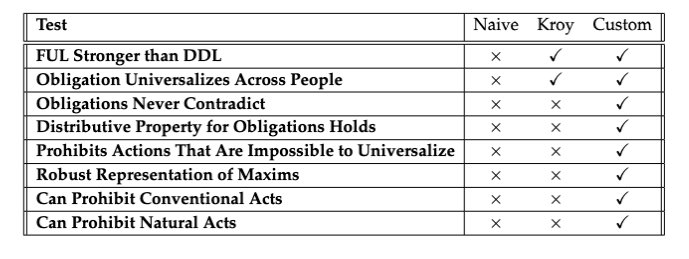
\includegraphics[scale=0.4]{goalstable.png}
\caption{Table showing which tests each implementation passes. The naive interpretation is raw DDL, 
Kroy is based on Moshe Kroy's formalization of the FUL, and the custom formalization is my novel implementation.} \label{table}
\end{figure}
%
\begin{isamarkuptext}%
\textbf{FUL Stronger than DDL} The FUL should not hold in raw DDL, which I use a control group. 
If the FUL holds in the base logic, then adding it as an axiom doesn't make the logic any stronger, 
which is troubling because the base logic does not come equipped with the categorical imperative built-in. It 
defines basic properties of obligation, such as ought implies can, but contains no axioms that represent
the formula of universal law. Therefore, if a formalization of the FUL holds in the 
base logic, then it is too weak to actually represent the FUL. Both Kroy's formalization
and my implementation do not hold in the base logic, and thus represent some progress over the control group.
To test this property, I used Nitpick to find a countermodel in which my version of the FUL does not hold. 
I performed this test before adding the FUL as an axiom, since after adding it no countermodel will
be possible.%
\end{isamarkuptext}\isamarkuptrue%
%
\begin{isamarkuptext}%
\medskip
\noindent \textbf{Obligation Universalizes Across People} The obligations prescribed by the Formula of Universal Law
should generalize across people. In other words, if a maxim is obligated for one person, it is obligated
for all other people because maxims are not person-specific. Velleman argues that, because 
reason is accessible to everyone identically, obligations apply to all people equually \citep[25]{velleman}. 
When Kant describes the categorical imperative as the objective principle of the will, he is referring 
to the fact that, as opposed to a subjective principle, the categorical imperative applies to all 
rational agents equally \citep[16]{groundwork}. At its core, the FUL best handles, ``the temptation 
to make oneself an exception: selfishness, meanness, advantagetaking, and disregard for the rights 
of others'' \citep[30]{KorsgaardFUL}. Kroy makes this property the center of his
formalization, which essentially says that if an act is permissible for someone, it is permissible for 
everyone.\footnote{Formally, $P\{A(s)\} \longrightarrow \forall p. P\{A(p)\}$} Kroy's interpretation and 
my interpretation satisfy this property, but the naive interpretation does not. Below I show how I 
ran this test for my interpreation.%
\end{isamarkuptext}\isamarkuptrue%
\isacommand{lemma}\isamarkupfalse%
\ wrong{\isacharunderscore}if{\isacharunderscore}wrong{\isacharunderscore}for{\isacharunderscore}someone{\isacharcolon}\isanewline
\ \ \isakeyword{shows}\ {\isachardoublequoteopen}{\isasymforall}w{\isachardot}\ {\isasymforall}c{\isacharcolon}{\isacharcolon}t{\isachardot}\ {\isasymforall}g{\isacharcolon}{\isacharcolon}t{\isachardot}\ {\isasymforall}a{\isachardot}\ {\isasymexists}s{\isacharcolon}{\isacharcolon}s{\isachardot}\ O{\isacharbraceleft}\isactrlbold {\isasymnot}\ {\isacharparenleft}W\ {\isacharparenleft}c{\isacharcomma}\ a{\isacharcomma}\ g{\isacharparenright}\ s{\isacharparenright}\ {\isacharbar}\ c{\isacharbraceright}\ w\ {\isasymlongrightarrow}\ {\isacharparenleft}{\isasymforall}p{\isachardot}\ \ O{\isacharbraceleft}\isactrlbold {\isasymnot}\ {\isacharparenleft}W\ {\isacharparenleft}c{\isacharcomma}\ a{\isacharcomma}\ g{\isacharparenright}\ p{\isacharparenright}\ {\isacharbar}\ c{\isacharbraceright}\ w{\isacharparenright}\ {\isachardoublequoteclose}\isanewline
%
\isadelimproof
\ \ %
\endisadelimproof
%
\isatagproof
\isacommand{by}\isamarkupfalse%
\ blast\isanewline
%
\isamarkupcmt{This lemma shows that if a maxim (c, a, g) is wrong for subject $s$ at a world, then it is wrong
for all people at $s$. Isabelle automatically completed this proof using the \texttt{blast} method, 
which implements a generic tableau prover, a proof method that operates on lists of formulae using 
rules for conjunction, disjunction, universal quantification, and existential quantification \citep{blast}.%
}%
\endisatagproof
{\isafoldproof}%
%
\isadelimproof
\isanewline
%
\endisadelimproof
\isanewline
\isacommand{lemma}\isamarkupfalse%
\ right{\isacharunderscore}if{\isacharunderscore}right{\isacharunderscore}for{\isacharunderscore}someone{\isacharcolon}\isanewline
\ \ \isakeyword{shows}\ {\isachardoublequoteopen}{\isasymforall}w{\isachardot}\ {\isasymforall}c{\isacharcolon}{\isacharcolon}t{\isachardot}\ {\isasymforall}g{\isacharcolon}{\isacharcolon}t{\isachardot}\ {\isasymexists}s{\isacharcolon}{\isacharcolon}s{\isachardot}\ O{\isacharbraceleft}W\ {\isacharparenleft}c{\isacharcomma}\ M{\isacharcomma}\ g{\isacharparenright}\ s\ {\isacharbar}\ c{\isacharbraceright}\ w\ {\isasymlongrightarrow}\ {\isacharparenleft}{\isasymforall}p{\isachardot}\ \ O{\isacharbraceleft}W\ {\isacharparenleft}c{\isacharcomma}\ M{\isacharcomma}\ g{\isacharparenright}\ p\ {\isacharbar}\ c{\isacharbraceright}\ w{\isacharparenright}\ {\isachardoublequoteclose}\isanewline
%
\isadelimproof
\ \ %
\endisadelimproof
%
\isatagproof
\isacommand{by}\isamarkupfalse%
\ blast\isanewline
%
\isamarkupcmt{This lemma shows that if a maxim (c, a, g) is right for subject $s$ at a world, then it is wrong
for all people at $s$. The proof similarly proceeds using \texttt{blast}. I represent my tests as 
lemmas, that I expect Isabelle to either prove or refute. The statement following the keyword \texttt{shows}
is the sentence of the lemma, and the proof follows the \texttt{by} keyword.%
}%
\endisatagproof
{\isafoldproof}%
%
\isadelimproof
%
\endisadelimproof
%
\begin{isamarkuptext}%
\noindent \textbf{Contradictory Obligations} DDL itself allows contradictory obligations, but contradictory obligations
make obeying the prescriptions of an ethical theory impossible.
Kant subscribes to the general, popular view that morality is supposed to guide action, so ought implies 
can\footnote{Kohl points out that this principle is referred to as 
Kant's dictum or Kant's law in the literature \citep[footnote 1]{kohl}.}. Kohl reconstructs his argument for the principle as 
follows: if the will cannot comply with the moral law, then the moral law has no prescriptive authority 
for the will \citep[703-4]{kohl}. This defeats the purpose of Kant's theory, which is to develop an unconditional, categorical imperative 
for rational agents. Ought implies can requires that obligations never contradict, because an agent 
can't perform contradictory actions. Therefore, any ethical theory that respects ought implies can, 
and Kantian ethics in particular, must not result in conflicting obligations. 
Kant only briefly discusses contradictory obligations in \emph{Metaphysics of Morals}, where he argues that 
conflicting moral obligations are impossible under his theory \citep[V224]{metaphysicsintro}. Particularly, the categorical imperative generates 
``strict negative laws of omission,'' which cannot conflict by definition \citep[45]{timmerman}.\footnote{The 
kinds of obligations generated by the FUL are called ``perfect duties'' which arise from ``contradictions 
in conception,'' or maxims that we cannot even concieve of universalizing. These duties are always negative 
and thus never conflict. Kant also presents ``imperfect duties,'' generated from ``contradictions in will,''
or maxims that we can concieve of universalizing but would never want to. These duties tend to be broader, 
such as ``improve oneself" or "help others," and are secondary to perfect duties. My project only analyzes 
perfect duties, as these are always stronger than imperfect duties.} Both the naive formalization and 
Kroy's formalization allow contradictory obligations, but I explicitly add an axiom to my formalization
that prohibits contradictory obligations.%
\end{isamarkuptext}\isamarkuptrue%
\isacommand{lemma}\isamarkupfalse%
\ conflicting{\isacharunderscore}obligations{\isacharcolon}\isanewline
\ \ \isakeyword{shows}\ {\isachardoublequoteopen}{\isasymnot}\ {\isacharparenleft}O{\isacharbraceleft}W\ {\isacharparenleft}c{\isacharcomma}\ a{\isacharcomma}\ g{\isacharparenright}\ s{\isacharbar}c{\isacharbraceright}\ \isactrlbold {\isasymand}\ O{\isacharbraceleft}\isactrlbold {\isasymnot}{\isacharparenleft}W\ {\isacharparenleft}c{\isacharcomma}\ a{\isacharcomma}\ g{\isacharparenright}\ s{\isacharparenright}{\isacharbar}\ c{\isacharbraceright}{\isacharparenright}\ w{\isachardoublequoteclose}\isanewline
%
\isadelimproof
\ \ %
\endisadelimproof
%
\isatagproof
\isacommand{using}\isamarkupfalse%
\ no{\isacharunderscore}contradictions\ \isacommand{by}\isamarkupfalse%
\ blast\isanewline
%
\isamarkupcmt{This test passes immediately by the new axiom that prohibits contradictory obligations.%
}%
\endisatagproof
{\isafoldproof}%
%
\isadelimproof
\isanewline
%
\endisadelimproof
\isanewline
\isacommand{lemma}\isamarkupfalse%
\ implied{\isacharunderscore}contradiction{\isacharcolon}\isanewline
\ \ \isakeyword{assumes}\ {\isachardoublequoteopen}{\isacharparenleft}{\isacharparenleft}{\isacharparenleft}W\ {\isacharparenleft}c{\isadigit{1}}{\isacharcomma}\ a{\isadigit{1}}{\isacharcomma}\ g{\isadigit{1}}{\isacharparenright}\ s{\isacharparenright}\ \isactrlbold {\isasymand}\ {\isacharparenleft}W\ {\isacharparenleft}c{\isadigit{2}}{\isacharcomma}\ a{\isadigit{2}}{\isacharcomma}\ g{\isadigit{2}}{\isacharparenright}\ s{\isacharparenright}{\isacharparenright}\ \isactrlbold {\isasymrightarrow}\ \isactrlbold {\isasymbottom}{\isacharparenright}\ w{\isachardoublequoteclose}\isanewline
\ \ \isakeyword{shows}\ {\isachardoublequoteopen}\isactrlbold {\isasymnot}\ {\isacharparenleft}O{\isacharbraceleft}W{\isacharparenleft}c{\isadigit{1}}{\isacharcomma}\ a{\isadigit{1}}{\isacharcomma}\ g{\isadigit{1}}{\isacharparenright}\ s{\isacharbar}c{\isacharbraceright}\ \isactrlbold {\isasymand}\ O{\isacharbraceleft}W{\isacharparenleft}c{\isadigit{2}}{\isacharcomma}\ a{\isadigit{2}}{\isacharcomma}\ g{\isadigit{2}}{\isacharparenright}\ s{\isacharbar}c{\isacharbraceright}{\isacharparenright}\ w{\isachardoublequoteclose}\isanewline
%
\isadelimproof
\ \ %
\endisadelimproof
%
\isatagproof
\isacommand{using}\isamarkupfalse%
\ assms\ no{\isacharunderscore}contradictions\ \isacommand{by}\isamarkupfalse%
\ blast\isanewline
%
\isamarkupcmt{This stronger property states that the combination of obligatory maxims can't
 imply a contradiction and should hold for the same reasons that contradictory obligations aren't
allowed. The added axiom also makes this test pass.%
}%
\endisatagproof
{\isafoldproof}%
%
\isadelimproof
%
\endisadelimproof
%
\begin{isamarkuptext}%
During testing, I also realized that contradictory obligations are closely related to two other properties
that also fail in both prior attempts. First is the idea that obligation implies permissibility, or 
that obligation is a stronger property than permissibility. If there are no contradictory obligations, 
then this property holds because actions are either permissible or prohibited and obligation contradicts
prohibition. Moreover, in a system with contradictory obligations, this property fails because there is some
A that is obligated but also prohibited and therefore not permisible. Formalizing this property below shows 
that this follows from the definition of implication in propositional logic.

\medskip%
\end{isamarkuptext}\isamarkuptrue%
\isacommand{lemma}\isamarkupfalse%
\ {\isachardoublequoteopen}{\isasymTurnstile}\ {\isacharparenleft}{\isacharparenleft}O\ {\isacharbraceleft}A{\isacharbraceright}\ \isactrlbold {\isasymand}\ O\ {\isacharbraceleft}\isactrlbold {\isasymnot}\ A{\isacharbraceright}{\isacharparenright}\ \isactrlbold {\isasymequiv}\ {\isacharparenleft}\isactrlbold {\isasymnot}\ {\isacharparenleft}O\ {\isacharbraceleft}A{\isacharbraceright}\ \isactrlbold {\isasymrightarrow}\ \isactrlbold {\isasymnot}\ O\ {\isacharbraceleft}\isactrlbold {\isasymnot}A{\isacharbraceright}{\isacharparenright}{\isacharparenright}{\isacharparenright}{\isachardoublequoteclose}\isanewline
%
\isadelimproof
\ \ %
\endisadelimproof
%
\isatagproof
\isacommand{by}\isamarkupfalse%
\ simp\isanewline
%
\isamarkupcmt{\texttt{simp} is the simplification tactic, which unfolds definitions to complete a proof. The 
left-hand side states that $A$ is both obligated and prohibited, and is equivalent to the right-hand side, 
which states that $A$ is obligated but not permissible.%
}%
\endisatagproof
{\isafoldproof}%
%
\isadelimproof
%
\endisadelimproof
%
\begin{isamarkuptext}%
\noindent \textbf{Distributive Property} Another property related to contradictory obligations is the distributive property for the obligation
operator.\footnote{Formally, $O\{A\} \wedge O\{B\} \longleftrightarrow O\{A \wedge B\}$.} This is 
another property that we expect to hold. The rough English translation of  $O \{ A \wedge B \} $ is ``you are obligated to 
do both A and B". The rough English translation of $O\{A\} \wedge O\{B\}$ is ``you are obligated to do A 
and you are obligated to do B." We think those English sentences mean the same thing, so they should mean 
the same thing in logic as well. Moreover, if that (rather intuitive) property holds, then contradictory
obligations are impossible, as shown in the below proof.%
\end{isamarkuptext}\isamarkuptrue%
\isacommand{lemma}\isamarkupfalse%
\ distributive{\isacharunderscore}implies{\isacharunderscore}no{\isacharunderscore}contradictions{\isacharcolon}\ \isanewline
\ \ \isakeyword{assumes}\ {\isachardoublequoteopen}{\isasymforall}A\ B{\isachardot}\ {\isasymTurnstile}\ {\isacharparenleft}{\isacharparenleft}O\ {\isacharbraceleft}A{\isacharbraceright}\ \isactrlbold {\isasymand}\ O\ {\isacharbraceleft}B{\isacharbraceright}{\isacharparenright}\ \isactrlbold {\isasymequiv}\ O\ {\isacharbraceleft}A\ \isactrlbold {\isasymand}\ B{\isacharbraceright}{\isacharparenright}{\isachardoublequoteclose}\isanewline
\ \ \isakeyword{shows}\ {\isachardoublequoteopen}{\isasymforall}A{\isachardot}\ {\isasymTurnstile}{\isacharparenleft}\ \isactrlbold {\isasymnot}{\isacharparenleft}O\ {\isacharbraceleft}A{\isacharbraceright}\ \isactrlbold {\isasymand}\ O\ {\isacharbraceleft}\isactrlbold {\isasymnot}\ A{\isacharbraceright}{\isacharparenright}{\isacharparenright}\ {\isachardoublequoteclose}\isanewline
%
\isadelimproof
\ \ %
\endisadelimproof
%
\isatagproof
\isacommand{using}\isamarkupfalse%
\ O{\isacharunderscore}diamond\ assms\ \isacommand{by}\isamarkupfalse%
\ blast\isanewline
%
\isamarkupcmt{The \texttt{assumes} keyword indicates assumptions used when proving a lemma. I use it here to 
capture the idea of metalogical implication. With the assumption, the lemma above reads, ``If the distributive
property holds in this logic, then obligations cannot contradict."%
}%
\endisatagproof
{\isafoldproof}%
%
\isadelimproof
%
\endisadelimproof
%
\begin{isamarkuptext}%
Again, this test fails in the naive formalization and for Kroy's formalization, but
passes for my interpretation because I require that obligations don't contradict as an axiom.%
\end{isamarkuptext}\isamarkuptrue%
\isacommand{lemma}\isamarkupfalse%
\ distribution{\isacharcolon}\isanewline
\ \ \isakeyword{assumes}\ {\isachardoublequoteopen}{\isasymTurnstile}\ {\isacharparenleft}O\ {\isacharbraceleft}A{\isacharbraceright}\ \isactrlbold {\isasymand}\ O\ {\isacharbraceleft}B{\isacharbraceright}{\isacharparenright}{\isachardoublequoteclose}\isanewline
\ \ \isakeyword{shows}\ {\isachardoublequoteopen}{\isasymTurnstile}\ O\ {\isacharbraceleft}A\ \isactrlbold {\isasymand}\ B{\isacharbraceright}{\isachardoublequoteclose}\isanewline
%
\isadelimproof
\ \ %
\endisadelimproof
%
\isatagproof
\isacommand{using}\isamarkupfalse%
\ assms\ no{\isacharunderscore}contradictions\ \isacommand{by}\isamarkupfalse%
\ fastforce\isanewline
%
\isamarkupcmt{Once again, the proof proceeds almost immediately using the new axiom.%
}%
\endisatagproof
{\isafoldproof}%
%
\isadelimproof
%
\endisadelimproof
%
\begin{isamarkuptext}%
\medskip 

\noindent \textbf{Un-universalizable Actions} Recall that under 
the logical contradiction interpretation of the Formula of Universal Law, it prohibits lying because, in a world 
where everyone simultaneously lies, lying is impossible. In other words, not everyone can simultaneously
lie because the institution of lying and believing would break down. In Section \nameref{praccon}, 
I recreated Korsgaard's argument for why the logical contradiction interpretation is weaker than what the
Formula of Universal Law should actually require. Therefore, any implementation of the FUL should be 
able to show that the actions prohibited by the logical contradiction interpretation are prohibited, 
because the actions prohibited by the practical contradiction interpretation are a superset of these.
The FUL should show that actions that cannot possibly be universalized are prohibited, because those acts cannot be willed in 
a world where they are universalized. This property fails to hold in both the naive formalization 
and Kroy's formalization, but holds for my custom formalization. Showing that this property holds
for my formalization required significant logical background is presented in Appendix \ref{weirdtests}%
\end{isamarkuptext}\isamarkuptrue%
%
\begin{isamarkuptext}%
\noindent \textbf{Maxims} Kant does not evaluate the correctness of acts, but rather of maxims. Therefore, any 
faithful formalization of the categorical imperative must evaluate maxims, not acts. This requires 
representing a maxim and making it the input to the obligation operator, which neither of the prior 
attempts do. Because my implementation includes the notion of a maxim, it is able to perform sophisticated 
reasoning as demonstrated in Sections \nameref{joking} and \nameref{murderer}. Staying faithful to the philosophical 
literature enables my system to make more reliable judgements.

\medskip%
\end{isamarkuptext}\isamarkuptrue%
%
\begin{isamarkuptext}%
\noindent \textbf{Conventional and Natural Acts} When arguing for the practical contradiction interpretation,
Korsgaard makes a distinction between conventional and natural acts \citep{KorsgaardFUL}. 
A conventional act like promising relies on a convention, like the 
convention that a promise is a commitment, whereas a natural act is possible simply because of the laws 
of the natural world. It is easier to show the wrongness of conventional acts because there are worlds 
in which these acts are impossible; namely, worlds in which the convention does not exist. For example, 
the common argument against falsely promising is that if everyone were to falsely promise, the convention 
of promising would fall apart because people wouldn't believe each other, so falsely promising is prohibited. 
It is more difficult to show the wrongness of a natural act, like murder or violence. These acts can 
never be logically impossible; even if everyone murders or acts violently, murder and violence will 
still be possible, so it is difficult to show that they violate the FUL. 

Both the naive and Kroy's interpretations fail to show the wrongness of conventional or natural acts. 
My system shows the wrongness of both natural and conventional acts because it is faithful to Korsgaard's 
practical contradiction interpretation of the FUL, which is the canonical interpretation of the 
FUL \citep{KorsgaardFUL}. This test passes due to the results shown in Chapter Applications, where I
use my system to reason about two ethical dilemmas, one which involves conventional acts and the other which
involves natural acts.%
\end{isamarkuptext}\isamarkuptrue%
%
\isadelimproof
%
\endisadelimproof
%
\isatagproof
%
\endisatagproof
{\isafoldproof}%
%
\isadelimproof
%
\endisadelimproof
%
\isadelimtheory
%
\endisadelimtheory
%
\isatagtheory
%
\endisatagtheory
{\isafoldtheory}%
%
\isadelimtheory
%
\endisadelimtheory
%
\end{isabellebody}%
\endinput
%:%file=~/Desktop/cs91r/paper/thesis_3_implementation.thy%:%
%:%24=6%:%
%:%36=8%:%
%:%37=9%:%
%:%38=10%:%
%:%39=11%:%
%:%40=12%:%
%:%49=14%:%
%:%61=16%:%
%:%62=17%:%
%:%63=18%:%
%:%64=19%:%
%:%73=21%:%
%:%85=23%:%
%:%86=24%:%
%:%87=25%:%
%:%88=26%:%
%:%89=27%:%
%:%91=29%:%
%:%92=29%:%
%:%93=29%:%
%:%96=31%:%
%:%97=32%:%
%:%98=33%:%
%:%99=34%:%
%:%100=35%:%
%:%101=36%:%
%:%102=37%:%
%:%103=38%:%
%:%104=39%:%
%:%105=40%:%
%:%106=41%:%
%:%108=43%:%
%:%109=43%:%
%:%111=44%:%
%:%112=45%:%
%:%113=46%:%
%:%114=47%:%
%:%115=48%:%
%:%116=49%:%
%:%117=50%:%
%:%118=51%:%
%:%126=53%:%
%:%138=55%:%
%:%139=56%:%
%:%140=57%:%
%:%141=58%:%
%:%142=59%:%
%:%143=60%:%
%:%144=61%:%
%:%145=62%:%
%:%146=63%:%
%:%147=64%:%
%:%148=65%:%
%:%149=66%:%
%:%150=67%:%
%:%151=68%:%
%:%152=69%:%
%:%153=70%:%
%:%154=71%:%
%:%155=72%:%
%:%156=73%:%
%:%157=74%:%
%:%158=75%:%
%:%159=76%:%
%:%160=77%:%
%:%161=78%:%
%:%162=79%:%
%:%164=82%:%
%:%165=82%:%
%:%167=83%:%
%:%168=84%:%
%:%169=85%:%
%:%170=86%:%
%:%171=87%:%
%:%172=88%:%
%:%173=89%:%
%:%174=90%:%
%:%177=92%:%
%:%178=93%:%
%:%179=94%:%
%:%180=95%:%
%:%181=96%:%
%:%182=97%:%
%:%183=98%:%
%:%184=99%:%
%:%185=100%:%
%:%186=101%:%
%:%187=102%:%
%:%188=103%:%
%:%189=104%:%
%:%190=105%:%
%:%191=106%:%
%:%192=107%:%
%:%193=108%:%
%:%194=109%:%
%:%195=110%:%
%:%196=111%:%
%:%197=112%:%
%:%198=113%:%
%:%199=114%:%
%:%200=115%:%
%:%201=116%:%
%:%202=117%:%
%:%203=118%:%
%:%204=119%:%
%:%205=120%:%
%:%206=121%:%
%:%207=122%:%
%:%208=123%:%
%:%209=124%:%
%:%210=125%:%
%:%211=126%:%
%:%212=127%:%
%:%213=128%:%
%:%214=129%:%
%:%215=130%:%
%:%216=131%:%
%:%217=132%:%
%:%218=133%:%
%:%219=134%:%
%:%220=135%:%
%:%221=136%:%
%:%222=137%:%
%:%223=138%:%
%:%224=139%:%
%:%225=140%:%
%:%226=141%:%
%:%227=142%:%
%:%228=143%:%
%:%229=144%:%
%:%230=145%:%
%:%231=146%:%
%:%232=147%:%
%:%233=148%:%
%:%234=149%:%
%:%235=150%:%
%:%236=151%:%
%:%237=152%:%
%:%238=153%:%
%:%239=154%:%
%:%240=155%:%
%:%242=157%:%
%:%243=157%:%
%:%244=158%:%
%:%246=159%:%
%:%247=160%:%
%:%248=161%:%
%:%249=162%:%
%:%257=164%:%
%:%269=166%:%
%:%270=167%:%
%:%271=168%:%
%:%272=169%:%
%:%273=170%:%
%:%274=171%:%
%:%275=172%:%
%:%276=173%:%
%:%277=174%:%
%:%278=175%:%
%:%279=176%:%
%:%280=177%:%
%:%281=178%:%
%:%282=179%:%
%:%283=180%:%
%:%284=181%:%
%:%285=182%:%
%:%286=183%:%
%:%287=184%:%
%:%288=185%:%
%:%289=186%:%
%:%290=187%:%
%:%291=188%:%
%:%292=189%:%
%:%293=190%:%
%:%294=191%:%
%:%295=192%:%
%:%296=193%:%
%:%297=194%:%
%:%298=195%:%
%:%299=196%:%
%:%300=197%:%
%:%301=198%:%
%:%302=199%:%
%:%303=200%:%
%:%304=201%:%
%:%305=202%:%
%:%306=203%:%
%:%307=204%:%
%:%308=205%:%
%:%309=206%:%
%:%310=207%:%
%:%311=208%:%
%:%312=209%:%
%:%313=210%:%
%:%314=211%:%
%:%315=212%:%
%:%316=213%:%
%:%317=214%:%
%:%318=215%:%
%:%319=216%:%
%:%321=219%:%
%:%322=219%:%
%:%323=220%:%
%:%325=221%:%
%:%326=222%:%
%:%329=224%:%
%:%330=225%:%
%:%331=226%:%
%:%332=227%:%
%:%333=228%:%
%:%334=229%:%
%:%335=230%:%
%:%336=231%:%
%:%337=232%:%
%:%338=233%:%
%:%339=234%:%
%:%340=235%:%
%:%341=236%:%
%:%342=237%:%
%:%343=238%:%
%:%344=239%:%
%:%345=240%:%
%:%346=241%:%
%:%347=242%:%
%:%348=243%:%
%:%349=244%:%
%:%350=245%:%
%:%351=246%:%
%:%353=249%:%
%:%354=249%:%
%:%355=250%:%
%:%357=251%:%
%:%358=252%:%
%:%359=252%:%
%:%362=258%:%
%:%363=259%:%
%:%364=260%:%
%:%365=261%:%
%:%366=262%:%
%:%367=263%:%
%:%368=264%:%
%:%369=265%:%
%:%370=266%:%
%:%371=267%:%
%:%372=268%:%
%:%373=269%:%
%:%374=270%:%
%:%375=271%:%
%:%377=273%:%
%:%378=273%:%
%:%379=274%:%
%:%381=275%:%
%:%384=277%:%
%:%385=278%:%
%:%386=279%:%
%:%387=280%:%
%:%388=281%:%
%:%389=282%:%
%:%390=283%:%
%:%391=284%:%
%:%392=285%:%
%:%393=286%:%
%:%394=287%:%
%:%395=288%:%
%:%396=289%:%
%:%397=290%:%
%:%398=291%:%
%:%399=292%:%
%:%400=293%:%
%:%401=294%:%
%:%402=295%:%
%:%403=296%:%
%:%404=297%:%
%:%405=298%:%
%:%406=299%:%
%:%407=300%:%
%:%408=301%:%
%:%409=302%:%
%:%410=303%:%
%:%411=304%:%
%:%412=305%:%
%:%413=306%:%
%:%414=307%:%
%:%415=308%:%
%:%416=309%:%
%:%417=310%:%
%:%418=311%:%
%:%419=312%:%
%:%420=313%:%
%:%421=314%:%
%:%422=315%:%
%:%424=317%:%
%:%425=317%:%
%:%426=318%:%
%:%428=319%:%
%:%429=320%:%
%:%430=320%:%
%:%431=321%:%
%:%432=322%:%
%:%433=322%:%
%:%434=323%:%
%:%436=324%:%
%:%437=325%:%
%:%440=327%:%
%:%441=328%:%
%:%442=329%:%
%:%443=330%:%
%:%445=332%:%
%:%446=332%:%
%:%447=333%:%
%:%449=334%:%
%:%450=335%:%
%:%451=335%:%
%:%452=336%:%
%:%453=337%:%
%:%454=337%:%
%:%456=338%:%
%:%457=339%:%
%:%458=340%:%
%:%466=342%:%
%:%478=344%:%
%:%479=345%:%
%:%480=346%:%
%:%481=347%:%
%:%483=350%:%
%:%484=350%:%
%:%486=351%:%
%:%487=352%:%
%:%488=353%:%
%:%489=354%:%
%:%492=356%:%
%:%493=357%:%
%:%495=359%:%
%:%496=359%:%
%:%498=359%:%
%:%502=359%:%
%:%503=359%:%
%:%504=360%:%
%:%505=360%:%
%:%506=360%:%
%:%515=362%:%
%:%516=363%:%
%:%517=364%:%
%:%518=365%:%
%:%519=366%:%
%:%520=367%:%
%:%521=368%:%
%:%522=369%:%
%:%523=370%:%
%:%524=371%:%
%:%525=372%:%
%:%526=373%:%
%:%527=374%:%
%:%528=375%:%
%:%529=376%:%
%:%530=377%:%
%:%531=378%:%
%:%532=379%:%
%:%533=380%:%
%:%534=381%:%
%:%535=382%:%
%:%536=383%:%
%:%538=385%:%
%:%539=385%:%
%:%540=386%:%
%:%542=387%:%
%:%543=388%:%
%:%546=390%:%
%:%548=392%:%
%:%549=392%:%
%:%550=393%:%
%:%552=394%:%
%:%553=395%:%
%:%554=395%:%
%:%555=396%:%
%:%556=397%:%
%:%557=397%:%
%:%558=398%:%
%:%559=398%:%
%:%561=398%:%
%:%565=398%:%
%:%566=398%:%
%:%568=399%:%
%:%569=400%:%
%:%570=401%:%
%:%571=402%:%
%:%572=403%:%
%:%573=404%:%
%:%583=406%:%
%:%584=407%:%
%:%585=408%:%
%:%586=409%:%
%:%587=410%:%
%:%588=411%:%
%:%589=412%:%
%:%590=413%:%
%:%591=414%:%
%:%592=415%:%
%:%593=416%:%
%:%594=417%:%
%:%595=418%:%
%:%596=419%:%
%:%597=420%:%
%:%598=421%:%
%:%599=422%:%
%:%600=423%:%
%:%601=424%:%
%:%603=426%:%
%:%604=426%:%
%:%606=428%:%
%:%607=429%:%
%:%608=430%:%
%:%609=431%:%
%:%610=432%:%
%:%619=434%:%
%:%631=436%:%
%:%632=437%:%
%:%633=438%:%
%:%634=439%:%
%:%635=440%:%
%:%636=441%:%
%:%637=442%:%
%:%638=443%:%
%:%639=444%:%
%:%640=445%:%
%:%641=446%:%
%:%642=447%:%
%:%643=448%:%
%:%644=449%:%
%:%645=450%:%
%:%646=451%:%
%:%647=452%:%
%:%648=453%:%
%:%649=454%:%
%:%652=458%:%
%:%653=459%:%
%:%654=460%:%
%:%655=461%:%
%:%656=462%:%
%:%657=463%:%
%:%660=465%:%
%:%661=466%:%
%:%662=467%:%
%:%663=468%:%
%:%664=469%:%
%:%665=470%:%
%:%666=471%:%
%:%667=472%:%
%:%668=473%:%
%:%669=474%:%
%:%673=476%:%
%:%674=477%:%
%:%675=478%:%
%:%676=479%:%
%:%677=480%:%
%:%678=481%:%
%:%679=482%:%
%:%680=483%:%
%:%681=484%:%
%:%682=485%:%
%:%683=486%:%
%:%684=487%:%
%:%685=488%:%
%:%686=489%:%
%:%688=491%:%
%:%689=491%:%
%:%690=492%:%
%:%693=493%:%
%:%697=493%:%
%:%698=493%:%
%:%700=494%:%
%:%701=495%:%
%:%702=496%:%
%:%703=497%:%
%:%709=497%:%
%:%712=498%:%
%:%713=499%:%
%:%714=499%:%
%:%715=500%:%
%:%718=501%:%
%:%722=501%:%
%:%723=501%:%
%:%725=502%:%
%:%726=503%:%
%:%727=504%:%
%:%728=505%:%
%:%738=507%:%
%:%739=508%:%
%:%740=509%:%
%:%741=510%:%
%:%742=511%:%
%:%743=512%:%
%:%744=513%:%
%:%745=514%:%
%:%746=515%:%
%:%747=516%:%
%:%748=517%:%
%:%749=518%:%
%:%750=519%:%
%:%751=520%:%
%:%752=521%:%
%:%753=522%:%
%:%754=523%:%
%:%755=524%:%
%:%756=525%:%
%:%757=526%:%
%:%758=527%:%
%:%760=529%:%
%:%761=529%:%
%:%762=530%:%
%:%765=531%:%
%:%769=531%:%
%:%770=531%:%
%:%771=531%:%
%:%773=532%:%
%:%779=532%:%
%:%782=533%:%
%:%783=534%:%
%:%784=534%:%
%:%785=535%:%
%:%786=536%:%
%:%789=537%:%
%:%793=537%:%
%:%794=537%:%
%:%795=537%:%
%:%797=538%:%
%:%798=539%:%
%:%799=540%:%
%:%809=542%:%
%:%810=543%:%
%:%811=544%:%
%:%812=545%:%
%:%813=546%:%
%:%814=547%:%
%:%815=548%:%
%:%816=549%:%
%:%817=550%:%
%:%819=553%:%
%:%820=553%:%
%:%823=554%:%
%:%827=554%:%
%:%828=554%:%
%:%830=555%:%
%:%831=556%:%
%:%832=557%:%
%:%842=559%:%
%:%843=560%:%
%:%844=561%:%
%:%845=562%:%
%:%846=563%:%
%:%847=564%:%
%:%848=565%:%
%:%850=567%:%
%:%851=567%:%
%:%852=568%:%
%:%853=569%:%
%:%856=570%:%
%:%860=570%:%
%:%861=570%:%
%:%862=570%:%
%:%864=571%:%
%:%865=572%:%
%:%866=573%:%
%:%876=575%:%
%:%877=576%:%
%:%879=578%:%
%:%880=578%:%
%:%881=579%:%
%:%882=580%:%
%:%885=581%:%
%:%889=581%:%
%:%890=581%:%
%:%891=581%:%
%:%893=582%:%
%:%903=584%:%
%:%904=585%:%
%:%905=586%:%
%:%906=587%:%
%:%907=588%:%
%:%908=589%:%
%:%909=590%:%
%:%910=591%:%
%:%911=592%:%
%:%912=593%:%
%:%913=594%:%
%:%914=595%:%
%:%915=596%:%
%:%916=597%:%
%:%920=601%:%
%:%921=602%:%
%:%922=603%:%
%:%923=604%:%
%:%924=605%:%
%:%925=606%:%
%:%926=607%:%
%:%927=608%:%
%:%931=611%:%
%:%932=612%:%
%:%933=613%:%
%:%934=614%:%
%:%935=615%:%
%:%936=616%:%
%:%937=617%:%
%:%938=618%:%
%:%939=619%:%
%:%940=620%:%
%:%941=621%:%
%:%942=622%:%
%:%943=623%:%
%:%944=624%:%
%:%945=625%:%
%:%946=626%:%
%:%947=627%:%
%:%948=628%:%
\newpage 
%
\begin{isabellebody}%
\setisabellecontext{thesis{\isacharunderscore}{\isadigit{4}}{\isacharunderscore}applications}%
%
\isadelimtheory
%
\endisadelimtheory
%
\isatagtheory
%
\endisatagtheory
{\isafoldtheory}%
%
\isadelimtheory
%
\endisadelimtheory
%
\isadelimdocument
%
\endisadelimdocument
%
\isatagdocument
%
\isamarkupsection{Applications \label{applications}%
}
\isamarkuptrue%
%
\endisatagdocument
{\isafolddocument}%
%
\isadelimdocument
%
\endisadelimdocument
%
\begin{isamarkuptext}%
In this chapter, I demonstrate that my system can produce correct judgements for challenging moral 
dilemmas that naive ethical reasoning cannot satisfactorily handle. Because my system is faithful to
philosophical literature, it can reproduce complex ethical judgements presented by philosophers as 
solutions to controversial open questions in ethics.
These dilemmas serve as examples of how my system could be used
in practice and demonstrate my system's ability to formalize longer, more complicted ethical arguments
than those presented in Chapter \ref{details}. Moreover, in the process of formalizing these dilemmas, 
I isolated the exact conditon that makes a maxim about lying wrong, an insight that could contribute to 
the philosophical literature on lying.

Many of the tests in Section \ref{testing} perform metaethical reasoning, which analyzes properties
of morality itself and involves questions about the nature of ethical truth. In this chapter, I perform
``applied ethical reasoning,'' which is the use of ethics to resolve dilemmas and make judgements about 
what an agent should or should not do. This is the kind of reasoning necessary for an AI agent using my system to
navigate the real world.

One challenge of applied ethical reasoning is that it requires more factual background than metaethical
reasoning. Because metaethics is about ethics itself, and not about the dilemmas that ethics is 
supposed to help us resolve, this kind of reasoning requires very little knowledge about the world. 
Applied ethical reasoning, on the other hand,
focuses on a particular ethical dilemma and thus requires enough factual background, or common sense, 
to understand the dilemma and options at hand. For example, an applied ethicist 
evaluating the permissibility of lying needs a robust definition of the term lying and likely some
understanding of communication and truth telling. Kantians specifically describe
this common sense as ``postulates of rationality'' that are nontrivial and nonnormative, but still
part of the process of practical reasoning itself \citep{silber}. 

In this chapter, I tackle this challenge by
endowing my system with this kind of common sense in the specific case of lying. My system needs common 
sense facts and definitions because, while it has the ability to reason
using the Formula of Universal Law, this reasoning must be applied to objects that are defined
using common sense. 

Because these common sense facts can determine my system's judgements, they are part of the trusted
code base for my system, or the logic and code that a user must trust in order to trust my system. 
Changing these common sense facts will change the judgements 
that my system makes. For example, if we define truth telling as an act that is self-contradictory (perhaps
by defining it as $p \wedge \neg p$), then my system will output that truth telling is prohibited.
Malicious common sense facts and definitions will result in bad ethical judgements. 
The challenge of endowing automated ethical reasoners with common sense reasoning is not unique to my 
system, and virtually all prior attempts in machine ethics face similar challenges.\footnote{See Section
\ref{relatedwork} for a survey of the common sense required in prior work.} Many prior attempts
sidestep this question, whereas I contribute an prototype implementation of one kind of common sense reasoning.

This chapter will provide examples of the kinds of common sense facts required to get my system
off the ground. I use a lean and uncontroversial common sense database
to achieve robust and powerful results. This serves as evidence for the ease of automating
Kantian ethics, an example of the additional work required to use my system in practice, and a 
demonstration of my system's power and flexibility. These examples demonstrate that, armed with nuanced 
common sense facts, my system can make sophisticated judgements faithful to philosophical literature.%
\end{isamarkuptext}\isamarkuptrue%
%
\isadelimdocument
%
\endisadelimdocument
%
\isatagdocument
%
\isamarkupsubsection{Lies and Jokes \label{joking}%
}
\isamarkuptrue%
%
\endisatagdocument
{\isafolddocument}%
%
\isadelimdocument
%
\endisadelimdocument
%
\begin{isamarkuptext}%
The moral status of lying is hotly debated in the Kantian literature. I focus on two dilemmas
presented in Korsgaard's ``Right to Lie,'' which 
examines Kant's prohibition on lying \citep{KorsgaardRTL}. She begins with the case of 
lying and joking. Many of Kant's critics argue that his prohibition on lies includes lies told in 
the context of a joke, which should be permissible. Korsgaard responds by arguing 
that there is a crucial difference between lying and joking: lies involve deception, but jokes do not. 
The purpose of a joke is amusement, which does not rely on the listener believing the story told. 
Given appropriate definitions of lies and jokes, my system shows that jokes are permissible but lies 
are not, demonstrating its power and flexibility. This section demonstrates how my system can be used 
in practice; it needs to be given some baseline common sense facts, but with those facts, it can make 
sophisticated judgements. Moreover, because my system is faithful to definitions found in philosophical 
literature, it can perform nuanced reasoning, demonstrating the value of faithful automated ethics. 

First, Korsgaard argues that the categorical imperative prohibits lies because they involve deception. 
When universalized, lies will no longer be believed, so lying could never be an effective way of achieving 
any goal when universalized. Korsgaard points out that ``we believe what is said to us in a given 
context because most of the time people in that context say what they really think'' \citep[4]{KorsgaardRTL}. 
In order to formalize this argument, I first need to define lying and formalize Korsgaard's argument 
about the basis of trust.

I define lying and trust in terms of belief. As in Section \ref{details}, I choose thin, or minimal,
definitions to reduce the potential for controversy in my system's factual background.%
\end{isamarkuptext}\isamarkuptrue%
\isacommand{consts}\isamarkupfalse%
\ believe{\isacharcolon}{\isacharcolon}{\isachardoublequoteopen}s{\isasymRightarrow}t{\isasymRightarrow}t{\isachardoublequoteclose}\ {\isacharparenleft}{\isachardoublequoteopen}{\isacharunderscore}\ believes\ {\isacharunderscore}{\isachardoublequoteclose}{\isacharparenright}\isanewline
%
\isamarkupcmt{\texttt{believe} is a constant that maps a subject and a term to another DDL term. For example, 
subject ``Sara'' might believe the term ``the sky is blue'' to create the sentence ``Sara believes
that the sky is blue,'' which can be true or false at a world.%
}%
\begin{isamarkuptext}%
Logicians and epistemologists develop and debate complex logics of belief and knowledge \citep{seplogicbelief}. 
I avoid this complexity by defining the concept of belief simply as a constant that maps a subject, term pair 
to a term. For the examples in this section, this choice suffices. 
I encode some minimal properties of belief below, but avoid any full definition of the term. 

Belief is useful to construct the idea of ``knowingly uttering a falsehood,'' a core component 
of both lying and joking.%
\end{isamarkuptext}\isamarkuptrue%
\isacommand{consts}\isamarkupfalse%
\ utter{\isacharcolon}{\isacharcolon}{\isachardoublequoteopen}s{\isasymRightarrow}t{\isasymRightarrow}t{\isachardoublequoteclose}\isanewline
%
\isamarkupcmt{\texttt{utter} also maps a subject and term to another DDL term. For example, the sentence ``Sara
utters, `I am hungry' '' is a DDL term that can be true or false at a world.%
}\isanewline
\isacommand{abbreviation}\isamarkupfalse%
\ utter{\isacharunderscore}falsehood{\isacharcolon}{\isacharcolon}{\isachardoublequoteopen}s{\isasymRightarrow}t{\isasymRightarrow}t{\isachardoublequoteclose}\ \isakeyword{where}\isanewline
\ \ {\isachardoublequoteopen}utter{\isacharunderscore}falsehood\ s\ t\ {\isasymequiv}\ \ {\isacharparenleft}utter\ s\ t{\isacharparenright}\ \isactrlbold {\isasymand}\ {\isacharparenleft}\isactrlbold {\isasymnot}\ t{\isacharparenright}{\isachardoublequoteclose}\isanewline
%
\isamarkupcmt{To utter a falsehood is to utter a statement that is false, or to utter $t$ when $\neg t$.%
}\isanewline
\isacommand{abbreviation}\isamarkupfalse%
\ knowingly{\isacharunderscore}utter{\isacharunderscore}falsehood{\isacharcolon}{\isacharcolon}{\isachardoublequoteopen}s{\isasymRightarrow}t{\isasymRightarrow}t{\isachardoublequoteclose}\ \isakeyword{where}\isanewline
\ \ {\isachardoublequoteopen}knowingly{\isacharunderscore}utter{\isacharunderscore}falsehood\ s\ t\ {\isasymequiv}\ {\isacharparenleft}utter{\isacharunderscore}falsehood\ s\ t{\isacharparenright}\ \isactrlbold {\isasymand}\ {\isacharparenleft}\isactrlbold {\isasymnot}\ {\isacharparenleft}believe\ s\ t{\isacharparenright}{\isacharparenright}{\isachardoublequoteclose}\isanewline
%
\isamarkupcmt{Sometimes we unknowingly utter falsehoods. For example, if I believe that the Earth is flat, then 
when I utter, ``the Earth is flat,'' I am unknowingly uttering a falsehood. This motivates defining
the idea of knowingly uttering a falsehood, which requires both uttering a falsehood and not believing 
your utterance. If I utter ``the Earth is flat,'' even though I know that the Earth is round, I am 
knowingly uttering a falsehood.%
}%
\begin{isamarkuptext}%
The above abbreviations are the core of my formalization of Korsgaard's definitions
of lying and joking. They are also relatively uncontroversial and encode little moral
or normative content. They say nothing about the moral status of uttering a falsehood, 
the agent's intention when making the utterance, or the conversational norms guiding the utterance. 
The complexities of a complete definition of lying or belief are 
unnecessary for Kantian ethics, and therefore for my system, to make moral judgements. 

Using the above definitions, I define lying. I characterize a maxim as involving a lie if 
the act requires knowingly uttering a falsehood and the end requires that some person $p$ believe 
the false statement $t$.%
\end{isamarkuptext}\isamarkuptrue%
\isacommand{abbreviation}\isamarkupfalse%
\ lie{\isacharcolon}{\isacharcolon}{\isachardoublequoteopen}maxim{\isasymRightarrow}bool{\isachardoublequoteclose}\ \isakeyword{where}\ \isanewline
{\isachardoublequoteopen}lie\ {\isasymequiv}\ {\isasymlambda}\ {\isacharparenleft}c{\isacharcomma}\ a{\isacharcomma}\ g{\isacharparenright}{\isachardot}\ {\isasymexists}t{\isachardot}\ {\isacharparenleft}a\ \isactrlbold {\isasymlongrightarrow}\ {\isacharparenleft}{\isasymlambda}s{\isachardot}\ knowingly{\isacharunderscore}utter{\isacharunderscore}falsehood\ s\ t{\isacharparenright}{\isacharparenright}\ {\isasymand}\ {\isacharparenleft}{\isasymexists}p{\isachardot}\ {\isasymforall}w{\isachardot}\ {\isacharparenleft}g\ \isactrlbold {\isasymrightarrow}\ {\isacharparenleft}believe\ p\ t{\isacharparenright}{\isacharparenright}\ w{\isacharparenright}{\isachardoublequoteclose}\isanewline
%
\isamarkupcmt{The abbreviation above maps a maxim to a boolean value that indicates if it is a lie.%
}%
\begin{isamarkuptext}%
To avoid unintentional wrongdoing, I focus on ``knowing lies,'' 
in which the speaker is aware that they are lying. It is uncontroversial that, in order for an act to be
a knowing lie, the speaker must utter a false statement that they do not believe. This also makes it 
easier to make moral judgements about the speaker's action, since they were, at the very least, aware
of their lie. The second half of
this definition requires that the goal of the lie is deception. This is inspired by  Korsgaard's interpretation 
of a lie. She understands a lie as a kind of falsehood that is usually effective \emph{because} it decieves
\citep[4]{KorsgaardRTL}. In my formalization, this means that the purpose or goal of the maxim must
involve decieving someone, or, in other words, that someone believe what the speaker knows to be a 
falsehood. 

With the above logical background, I automate Korsgaard's argument that maxims that involve
lying are prohibited. First, I define the relevant subject and maxim.%
\end{isamarkuptext}\isamarkuptrue%
\isacommand{consts}\isamarkupfalse%
\ me{\isacharcolon}{\isacharcolon}s\isanewline
%
\isamarkupcmt{I am trying to reason about \emph{my} obligations so I will define myself as a specific subject. Again,
this is a minimal definition that does not include any facts about me, such as the fact that my name is
Lavanya or that I have brown hair.%
}\isanewline
\isacommand{consts}\isamarkupfalse%
\ m{\isacharcolon}{\isacharcolon}maxim\isanewline
%
\isamarkupcmt{I also define a maxim $m$. My goal is to show that if $m$ is a maxim about lying, then $m$
is prohibited.%
}\isanewline
\isacommand{consts}\isamarkupfalse%
\ c{\isacharcolon}{\isacharcolon}t\ a{\isacharcolon}{\isacharcolon}os\ g{\isacharcolon}{\isacharcolon}t\isanewline
%
\isamarkupcmt{$m$ will be composed of the circumstances, act, and goal above.%
}%
\begin{isamarkuptext}%
In the following lemma, I use my system to show that lying is prohibited. The assumptions of 
this lemma represent the common sense necessary to reach this conclusion. This
common sense background is a direct formalization of the premises of Korsgaard's argument. Using these
relatively minimal premises about individual behavior, my system derives a prohibition against lying.%
\end{isamarkuptext}\isamarkuptrue%
\isacommand{lemma}\isamarkupfalse%
\ lying{\isacharunderscore}prohibited{\isacharcolon}\isanewline
\ \ \isakeyword{assumes}\ {\isachardoublequoteopen}m\ {\isasymequiv}\ {\isacharparenleft}c{\isacharcolon}{\isacharcolon}t{\isacharcomma}\ a{\isacharcolon}{\isacharcolon}os{\isacharcomma}\ g{\isacharcolon}{\isacharcolon}t{\isacharparenright}{\isachardoublequoteclose}\isanewline
\ \ \isakeyword{assumes}\ {\isachardoublequoteopen}{\isasymforall}w{\isachardot}\ {\isasymforall}s{\isachardot}\ well{\isacharunderscore}formed\ m\ s\ w{\isachardoublequoteclose}\isanewline
%
\isamarkupcmt{Initial technical set-up: $m$ is a well-formed maxim composed of some circumstances, act, and goal.%
}\isanewline
\ \ \isakeyword{assumes}\ {\isachardoublequoteopen}lie\ m{\isachardoublequoteclose}\isanewline
%
\isamarkupcmt{$m$ is a maxim about lying as defined above. Precisely, it is a maxim in which the action requires 
knowingly uttering a falsehood and the goal requires that someone believe this falsehood.%
}\isanewline
\ \ \isakeyword{assumes}\ {\isachardoublequoteopen}{\isasymforall}t\ w{\isachardot}\ {\isacharparenleft}{\isacharparenleft}{\isasymforall}p{\isachardot}\ utter{\isacharunderscore}falsehood\ p\ t\ w{\isacharparenright}\ {\isasymlongrightarrow}\ {\isacharparenleft}{\isasymforall}p{\isachardot}\ \isactrlbold {\isasymnot}\ {\isacharparenleft}believe\ p\ t{\isacharparenright}\ w{\isacharparenright}{\isacharparenright}{\isachardoublequoteclose}\isanewline
%
\isamarkupcmt{Assumption that if everyone utters false statement $t$, then no one will believe $t$. This assumption is 
Korsgaard's core piece of ``common sense'' about lying \cite[5]{KorsgaardRTL}. This simple assumption encodes the common sense knowledge
that human communication involves an implicit trust, and that when this trust erodes, the convention of 
communication begins to break down and people no longer believe each other. Call this the ``convention of 
trust'' fact. In the rest of this section, I will test versions of this assumption, effectively encoding 
different common sense understandings of lying.%
}\isanewline
\ \ \isakeyword{assumes}\ {\isachardoublequoteopen}{\isasymforall}w{\isachardot}\ c\ w{\isachardoublequoteclose}\isanewline
%
\isamarkupcmt{Restrict our focus to worlds in which the circumstances hold. A technical detail.%
}\isanewline
\ \ \isakeyword{shows}\ {\isachardoublequoteopen}{\isasymTurnstile}\ {\isacharparenleft}prohibited\ m\ me{\isacharparenright}{\isachardoublequoteclose}\isanewline
%
\isadelimproof
%
\endisadelimproof
%
\isatagproof
\isacommand{proof}\isamarkupfalse%
\ {\isacharminus}\ \isanewline
\ \ \isacommand{have}\isamarkupfalse%
\ {\isachardoublequoteopen}{\isacharparenleft}{\isasymforall}p\ w{\isachardot}\ {\isacharparenleft}W\ m\ p{\isacharparenright}\ w{\isacharparenright}\ {\isasymlongrightarrow}\ {\isacharparenleft}{\isasymTurnstile}\ {\isacharparenleft}c\ \isactrlbold {\isasymrightarrow}\ {\isacharparenleft}\isactrlbold {\isasymnot}\ g{\isacharparenright}{\isacharparenright}{\isacharparenright}{\isachardoublequoteclose}\isanewline
\ \ \ \ \isacommand{by}\isamarkupfalse%
\ {\isacharparenleft}smt\ assms{\isacharparenleft}{\isadigit{1}}{\isacharparenright}\ assms{\isacharparenleft}{\isadigit{2}}{\isacharparenright}\ assms{\isacharparenleft}{\isadigit{5}}{\isacharparenright}\ case{\isacharunderscore}prod{\isacharunderscore}beta\ fst{\isacharunderscore}conv\ old{\isachardot}prod{\isachardot}exhaust\ snd{\isacharunderscore}conv{\isacharparenright}\isanewline
%
\isamarkupcmt{This proof requires some manual work. After I divide the proof into the intermediate steps shown 
here, Isabelle is able to do 
the rest. This step says that if $m$ is universalized, then the circumstances won't lead to the goal, 
which is close to the idea of the maxim not being universalizable.%
}\isanewline
\ \ \isacommand{have}\isamarkupfalse%
\ {\isachardoublequoteopen}not{\isacharunderscore}universalizable\ m\ me{\isachardoublequoteclose}\isanewline
\ \ \ \ \isacommand{by}\isamarkupfalse%
\ {\isacharparenleft}metis\ {\isacharparenleft}mono{\isacharunderscore}tags{\isacharcomma}\ lifting{\isacharparenright}\ assms{\isacharparenleft}{\isadigit{1}}{\isacharparenright}\ assms{\isacharparenleft}{\isadigit{2}}{\isacharparenright}\ case{\isacharunderscore}prod{\isacharunderscore}beta\ fst{\isacharunderscore}conv\ snd{\isacharunderscore}conv{\isacharparenright}\isanewline
\ \ \isacommand{thus}\isamarkupfalse%
\ {\isacharquery}thesis\isanewline
\ \ \ \ \isacommand{using}\isamarkupfalse%
\ FUL\ assms{\isacharparenleft}{\isadigit{2}}{\isacharparenright}\ \isacommand{by}\isamarkupfalse%
\ blast\ \isanewline
%
\isamarkupcmt{$?thesis$ is Isabelle's syntax for the goal of the lemma. In this case, $?thesis$ is equivalent to 
$\vDash prohibited \; m \; me$.%
}\isanewline
\isacommand{qed}\isamarkupfalse%
%
\endisatagproof
{\isafoldproof}%
%
\isadelimproof
%
\endisadelimproof
%
\begin{isamarkuptext}%
The lemma above demonstrates that my system finds that lying is prohibited with a thin definition
of lying and relatively uncontroversial facts about the world. My system needs two pieces of common 
sense to complete this proof. First, I defined lying as knowingly uttering a falsehood with the goal 
that someone believe the falsehood, a definition of lying that is relatively well-accepted. Second, I 
assumed (following in Korsgaard's footsteps) that if 
everyone lies in a given context, then people will stop believing each other in that context. This is 
a slightly heavier assumption, but it is still so uncontroversial that Korsgaard doesn't bother to justify
it in her argument against lying \citep{KorsgaardRTL}. 

Now that I have formalized Korsgaard's argument for why lying is prohibited, I will
implement her argument for why jokes are permissible. Specifically, she defines a joke as a story that is 
false and argues that joking is permissible because ``the universal practice of lying in the context of jokes
does not interfere with the purpose of jokes, which is to amuse and does not depend on
deception'' \citep[4]{KorsgaardRTL}. I use the fact that a joke does not depend on deception as the 
defining feature of a joke.%
\end{isamarkuptext}\isamarkuptrue%
\isacommand{abbreviation}\isamarkupfalse%
\ joke{\isacharcolon}{\isacharcolon}{\isachardoublequoteopen}maxim{\isasymRightarrow}bool{\isachardoublequoteclose}\ \isakeyword{where}\ \isanewline
{\isachardoublequoteopen}joke\ {\isasymequiv}\ {\isasymlambda}\ {\isacharparenleft}c{\isacharcomma}\ a{\isacharcomma}\ g{\isacharparenright}{\isachardot}\ \ {\isasymexists}t{\isachardot}\ {\isacharparenleft}a\ \isactrlbold {\isasymlongrightarrow}\ {\isacharparenleft}{\isasymlambda}s{\isachardot}\ knowingly{\isacharunderscore}utter{\isacharunderscore}falsehood\ s\ t{\isacharparenright}{\isacharparenright}\ {\isasymand}\ {\isasymnot}\ {\isacharparenleft}{\isasymexists}p{\isachardot}\ {\isasymforall}w{\isachardot}\ {\isacharparenleft}g\ \isactrlbold {\isasymrightarrow}\ {\isacharparenleft}believe\ p\ t{\isacharparenright}{\isacharparenright}\ w{\isacharparenright}{\isachardoublequoteclose}\isanewline
%
\isamarkupcmt{Thie abbreviation states that a maxim is a joke if the action involves knowingly uttering a falsehood but
the goal does \emph{not} require that someone believe the falsehood told.%
}%
\begin{isamarkuptext}%
This definition of a joke defines a joke as a falsehood uttered for some purpose that 
doesn't require deception, where deception involves someone believing the uttered falsehood. 
This definition doesn't require any conception of humor, but merely
distinguishes jokes from lies. 

Korsgaard argues that her above argument for a prohibition against lying also implies that joking is 
permissible, because its purpose is not to decieve, but something else entirely. This means that, 
even armed with the same convention of trust assumption as above, joking should be permissible. The 
lemma below shows exactly that.%
\end{isamarkuptext}\isamarkuptrue%
\isacommand{lemma}\isamarkupfalse%
\ joking{\isacharunderscore}not{\isacharunderscore}prohibited{\isacharcolon}\isanewline
\ \ \isakeyword{assumes}\ {\isachardoublequoteopen}m\ {\isasymequiv}\ {\isacharparenleft}c{\isacharcolon}{\isacharcolon}t{\isacharcomma}\ a{\isacharcolon}{\isacharcolon}os{\isacharcomma}\ g{\isacharcolon}{\isacharcolon}t{\isacharparenright}{\isachardoublequoteclose}\isanewline
\ \ \isakeyword{assumes}\ {\isachardoublequoteopen}{\isasymforall}w{\isachardot}\ {\isasymforall}s{\isachardot}\ well{\isacharunderscore}formed\ m\ s\ w{\isachardoublequoteclose}\isanewline
%
\isamarkupcmt{Initial set-up: $m$ is a well-formed maxim composed of some circumstances, act, and goal.%
}\isanewline
\ \ \isakeyword{assumes}\ {\isachardoublequoteopen}joke\ m{\isachardoublequoteclose}\isanewline
%
\isamarkupcmt{$m$ is a maxim about joking. Precisely, it is a maxim in which the action is to knowingly utter a 
falsehood and the goal does not require that someone believe this falsehood.%
}\isanewline
\ \ \isakeyword{assumes}\ {\isachardoublequoteopen}{\isasymforall}t\ w{\isachardot}\ {\isacharparenleft}{\isacharparenleft}{\isasymforall}p{\isachardot}\ utter{\isacharunderscore}falsehood\ p\ t\ w{\isacharparenright}\ {\isasymlongrightarrow}\ {\isacharparenleft}{\isasymforall}p{\isachardot}\ \isactrlbold {\isasymnot}\ {\isacharparenleft}believe\ p\ t{\isacharparenright}\ w{\isacharparenright}{\isacharparenright}{\isachardoublequoteclose}\isanewline
%
\isamarkupcmt{The same convention of trust assumption as in the above example.%
}\isanewline
\ \ \isakeyword{assumes}\ {\isachardoublequoteopen}{\isasymforall}w{\isachardot}\ c\ w{\isachardoublequoteclose}\isanewline
%
\isamarkupcmt{Restrict our focus to worlds in which the circumstances hold. A technical detail.%
}\isanewline
\ \ \isakeyword{shows}\ {\isachardoublequoteopen}{\isasymTurnstile}\ {\isacharparenleft}permissible\ m\ me{\isacharparenright}{\isachardoublequoteclose}\isanewline
%
\isadelimproof
\ \ %
\endisadelimproof
%
\isatagproof
\isacommand{by}\isamarkupfalse%
\ {\isacharparenleft}smt\ assms{\isacharparenleft}{\isadigit{1}}{\isacharparenright}\ assms{\isacharparenleft}{\isadigit{2}}{\isacharparenright}\ assms{\isacharparenleft}{\isadigit{3}}{\isacharparenright}\ case{\isacharunderscore}prod{\isacharunderscore}conv{\isacharparenright}\isanewline
%
\isamarkupcmt{Isabelle is able to show that maxims about joking are permissible. It also lists the facts used 
in its proof, which offer insight into how it arrived at its judgement. Specifically, it uses assumptions 1, 
2, and 3, which are the logical background and definition of the joking maxim. Notably, it does not use the 
convention of trust assumption. This demonstrates that even the convention of trust assumption is not
strong enough to prohibit joking, which is exactly the desired result.%
}%
\endisatagproof
{\isafoldproof}%
%
\isadelimproof
%
\endisadelimproof
%
\begin{isamarkuptext}%
My system shows that lies are prohibited and jokes are permissible with thin 
conceptions of amusement and deception. This shows that it isolates a necessary and sufficient property 
of this class of maxims that fail the universalizability test. My definitions of a lie and joke
only differ in whether or not their goal requires that someone believe the falsehood in question, so
this is a necessary and sufficient condition for a maxim about knowingly uttering falsehoods to be prohibited.
This logical fact derived by my system tracks a fact implicit in Korsgaard's argument and in most Kantian accounts
of lying: the wrongness of lying is derived from the requirement that someone believe the falsehood. 
The logical reality that this property is necessary and sufficient to generate a prohibition reflects
a deep philosohopical explanation of \emph{why} certain maxims about uttering falsehood fail the universalizability
test. Universalizing uttering a falsehood makes belief in that 
falsehood impossible, so any maxims with goals that require believing in the falsehood will be prohibited.

This account not only describes the kind of maxims that fail or pass the universalizability test, but it 
also provides a guide to constructing permissible maxims about uttering falsehoods. As an example, 
consider the idea of throwing a surprise birthday party. At first glance, the maxim of action is 
something like, ``When it is my friend's birthday, I will secretly plan a party so that I can surprise
them.'' The goal ``so that I can surprise them'' clearly requires that your friend believe the falsehood that 
you are not planning a party, else the surprise would be ruined. This seems to imply that 
Kantian ethics would prohibit surprise parties, which is a sad conclusion for birthday-lovers everywhere. 
Knowing that this maxim is prohibited because the goal requires belief
in a falsehood provides a way to rescue surprise parties. When throwing a 
surprise party, the objective is \emph{not} to surprise your friend, but to celebrate
your friend and help them have a fun birthday. If someone ruins the surprise, but the party is still fun
and the birthday person feels loved, then such a party is a success! Someone who
calls this party a failure is clearly missing the point of a surprise party. The goal of 
a surprise party is not the surprise itself, but rather celebrating the birthday person. The modified
goal\footnote{Some may worry that this argument implies that the ``means justify the ends,'' or that modifying
an act's goal can change its moral worth. This conclusion is not only unsurprising to Kantians, but it is the
defining feature of their theory. Under Kantian ethics, an action alone is not the kind of thing that can 
be moral or immoral; rather, a maxim, or a circumstances, act, goal tuple, is what has moral worth. The rightness 
of an action can hinge on the maxim's goal, circumstances, or act because these three features
of an action are inseparable.} no longer requires belief in the falsehood and thus passes the 
universalizability test. 

There are two implications of this section. First, my system is capable of performing ethical reasoning
sophisticated enough to show that lying is prohibited but joking is not. This is a direct consequence 
of my system's use of a robust conception of a maxim, which encodes the goal of an act as part of the 
maxim being evaluated. Because my implementation is faithful to philosophical literature, it is able 
to recreate Korsgaard's solution to a complex ethical dilemma that philosophers debated for decades. Second, 
in the process of making this argument precise, my system isolated a necessary and sufficient condition 
of a maxim about uttering a falsehood being prohibited: that the goal require that someone believe
the falsehood. This condition, made an long-standing argument in Kantian ethics more precise, can guide 
the correct formulation of future maxims, and could contribute to the rich philosophical conversation
about the wrongness of lying. In other words, an insight generated by the
computer provides value to ethicists, bolstering the argument for computational ethics provided in 
Section \ref{computationalethics}.%
\end{isamarkuptext}\isamarkuptrue%
%
\isadelimdocument
%
\endisadelimdocument
%
\isatagdocument
%
\isamarkupsubsection{Lying to a Liar \label{murderer}%
}
\isamarkuptrue%
%
\endisatagdocument
{\isafolddocument}%
%
\isadelimdocument
%
\endisadelimdocument
%
\begin{isamarkuptext}%
My system can not only distinguish between lying and joking, but it can also resolve the paradox of 
the murderer at the door. In this dilemma, murderer Bill knocks on your door asking about Sara, his 
intended victim. Sara is at home, but moral intuition says that you should lie to Bill and say 
that she is out to prevent him from murdering her. Many critics of Kantian ethics argue that the 
FUL prohibits you from lying in this instance; if everyone lied to murderers, then murderers wouldn't 
believe the lies and would search the house anyways. Korsgaard resolved this centuries-long debate by 
noting that the maxim of lying to a murderer is actually that of lying to a liar: Bill cannot 
announce his intentions to murder; instead, he must ``must suppose that you do not know who he is 
and what he has in mind'' \citep{KorsgaardRTL}.\footnote{Korsgaard assumes that the murderer will 
lie about his identity in order to take advantage of your honesty to find his victim. In footnote 5, 
she accepts that her arguments will not apply in the case of the honest murderer 
who announces his intentions, so she restricts her focus to the case of lying to a liar. She claims 
that in the case of the honest murderer, the correct act is to refuse to respond. Since I am formalizing
Korsgaard's argument, I also accept this assumption.} Thus, the maxim 
in question specifies that when someone lies to you, you are allowed to lie to them. The maxim of 
lying to the murderer is actually the maxim of lying to a liar, which is permissible. 

In this section, I formalize Korsgaard's argument for the permissibility of lying to a liar. First, I define
Bill's maxim, which is to hide his intention to murder.%
\end{isamarkuptext}\isamarkuptrue%
\isacommand{consts}\isamarkupfalse%
\ murderer{\isacharcolon}{\isacharcolon}s\isanewline
%
\isamarkupcmt{This example involves the murderer as an additional subject.%
}\isanewline
\isacommand{consts}\isamarkupfalse%
\ not{\isacharunderscore}a{\isacharunderscore}murderer{\isacharcolon}{\isacharcolon}t\isanewline
%
\isamarkupcmt{This statement represents the lie that the murderer tells you. By not announcing his
intention, he is implicitly telling you that he is not a murderer, as people normally assume that 
those knocking on their door are not murderers.%
}\isanewline
\isacommand{consts}\isamarkupfalse%
\ when{\isacharunderscore}at{\isacharunderscore}my{\isacharunderscore}door{\isacharcolon}{\isacharcolon}t\isanewline
%
\isamarkupcmt{These are the circumstances that the murderer is in.%
}\isanewline
\isacommand{consts}\isamarkupfalse%
\ find{\isacharunderscore}victim{\isacharcolon}{\isacharcolon}t\isanewline
%
\isamarkupcmt{This will be the murderer's goal: to find his victim.%
}\isanewline
\isacommand{abbreviation}\isamarkupfalse%
\ murderers{\isacharunderscore}maxim{\isacharcolon}{\isacharcolon}{\isachardoublequoteopen}maxim{\isachardoublequoteclose}\ \isakeyword{where}\ \isanewline
{\isachardoublequoteopen}murderers{\isacharunderscore}maxim\ {\isasymequiv}\ {\isacharparenleft}when{\isacharunderscore}at{\isacharunderscore}my{\isacharunderscore}door{\isacharcomma}\ {\isasymlambda}s{\isachardot}\ knowingly{\isacharunderscore}utter{\isacharunderscore}falsehood\ s\ not{\isacharunderscore}a{\isacharunderscore}murderer{\isacharcomma}\ find{\isacharunderscore}victim{\isacharparenright}{\isachardoublequoteclose}\isanewline
%
\isamarkupcmt{Using the above definitions, I can define the murderer's maxim as, ``When at your door, I will knowingly
utter the falsehood that I am not a murderer in order to find my intended victim.''%
}%
\begin{isamarkuptext}%
These constants are defined only in relation to each other and elide most of the complex features
of murder, life, and death. These thin representations will suffice to show
the wrongness of the murderer's maxim. Similarly, I can use thin representations to define your
maxim of lying about Sara's whereabouts.%
\end{isamarkuptext}\isamarkuptrue%
\isacommand{consts}\isamarkupfalse%
\ victim{\isacharunderscore}not{\isacharunderscore}home{\isacharcolon}{\isacharcolon}t\isanewline
%
\isamarkupcmt{This statement is the lie that you tell the murderer: that his intended victim is not at home.%
}\isanewline
\isacommand{abbreviation}\isamarkupfalse%
\ murderer{\isacharunderscore}at{\isacharunderscore}door{\isacharcolon}{\isacharcolon}t\ \isakeyword{where}\ \isanewline
{\isachardoublequoteopen}murderer{\isacharunderscore}at{\isacharunderscore}door\ {\isasymequiv}\ W\ murderers{\isacharunderscore}maxim\ murderer{\isachardoublequoteclose}\isanewline
%
\isamarkupcmt{These are the circumstances that you are in: the murderer has willed his maxim and thus lied to you.%
}\isanewline
\isacommand{consts}\isamarkupfalse%
\ protect{\isacharunderscore}victim{\isacharcolon}{\isacharcolon}t\isanewline
%
\isamarkupcmt{Your goal is to protect the murderer's intended victim.%
}\isanewline
\isacommand{abbreviation}\isamarkupfalse%
\ my{\isacharunderscore}maxim{\isacharcolon}{\isacharcolon}maxim\ \isakeyword{where}\ \isanewline
{\isachardoublequoteopen}my{\isacharunderscore}maxim\ {\isasymequiv}\ {\isacharparenleft}murderer{\isacharunderscore}at{\isacharunderscore}door{\isacharcomma}\ \ {\isasymlambda}s{\isachardot}\ knowingly{\isacharunderscore}utter{\isacharunderscore}falsehood\ s\ victim{\isacharunderscore}not{\isacharunderscore}home{\isacharcomma}\ protect{\isacharunderscore}victim{\isacharparenright}{\isachardoublequoteclose}\isanewline
%
\isamarkupcmt{Using these definitions, I construct your maxim, which is ``When a murderer is at my door, I will 
knowingly utter the falsehood that his intended victim is not at home, in order to protect the victim.''%
}%
\isadelimproof
%
\endisadelimproof
%
\isatagproof
%
\endisatagproof
{\isafoldproof}%
%
\isadelimproof
%
\endisadelimproof
%
\begin{isamarkuptext}%
I now formalize Korsgaard's argument for the permissibility of lying to a liar. She modifies
the convention of trust assumption above when she argues that, if the murderer believes that you don't 
believe he is a murderer, he will think that you won't lie to him. Precisely, she claims that, 
``it is because the murderer supposes you do not know what circumstances you are in - that is, that 
you do not know you are addressing a murderer - and so does not conclude from the fact that people 
in those circumstances always lie that you will lie'' \cite[6]{KorsgaardRTL}. Even though the maxim of 
lying to a murderer is universalized, Bill thinks that you don't know his true identity. Thus,
even if you have willed this maxim, he thinks that you won't perform the act of lying to the murderer,
since he thinks that you don't think you're in the relevant circumstances. I formalize this argument below.%
\end{isamarkuptext}\isamarkuptrue%
\isacommand{lemma}\isamarkupfalse%
\ lying{\isacharunderscore}to{\isacharunderscore}liar{\isacharunderscore}permissible{\isacharcolon}\isanewline
\ \ \isakeyword{assumes}\ {\isachardoublequoteopen}{\isasymTurnstile}\ {\isacharparenleft}well{\isacharunderscore}formed\ murderers{\isacharunderscore}maxim\ murderer{\isacharparenright}{\isachardoublequoteclose}\isanewline
\ \ \isakeyword{assumes}\ {\isachardoublequoteopen}{\isasymTurnstile}\ {\isacharparenleft}well{\isacharunderscore}formed\ my{\isacharunderscore}maxim\ me{\isacharparenright}{\isachardoublequoteclose}\isanewline
%
\isamarkupcmt{Initial set-up: both maxims are well-formed.%
}\isanewline
\ \ \isakeyword{assumes}\ {\isachardoublequoteopen}{\isasymTurnstile}\ {\isacharparenleft}protect{\isacharunderscore}victim\ \isactrlbold {\isasymrightarrow}\ {\isacharparenleft}murderer\ believes\ victim{\isacharunderscore}not{\isacharunderscore}home{\isacharparenright}{\isacharparenright}{\isachardoublequoteclose}\isanewline
%
\isamarkupcmt{In order for you to protect the victim, the murderer must believe that the victim is not home.%
}\isanewline
\ \ \isakeyword{assumes}\ {\isachardoublequoteopen}{\isasymforall}sentence{\isacharcolon}{\isacharcolon}t{\isachardot}\ {\isasymforall}p{\isadigit{1}}{\isacharcolon}{\isacharcolon}s{\isachardot}\ {\isasymforall}p{\isadigit{2}}{\isacharcolon}{\isacharcolon}s{\isachardot}\ {\isasymforall}w{\isacharcolon}{\isacharcolon}i{\isachardot}\ {\isacharparenleft}{\isacharparenleft}p{\isadigit{1}}\ believes\ {\isacharparenleft}utter{\isacharunderscore}falsehood\ p{\isadigit{2}}\ sentence{\isacharparenright}{\isacharparenright}\ w{\isacharparenright}\ {\isasymlongrightarrow}\ {\isacharparenleft}{\isasymnot}\ {\isacharparenleft}p{\isadigit{1}}\ believes\ sentence{\isacharparenright}\ w{\isacharparenright}{\isachardoublequoteclose}\isanewline
%
\isamarkupcmt{This is one of two assumptions that encode Korsgaard's core argument. If $p1$ believes that $p2$ 
utters a sentence as a falsehood, then $p1$ won't believe that sentence. This is a modification of the 
convention of trust assumption from above, and I will refer to it as the ``convention of belief" assumption.
Again, like the convention of trust assumption, this assumption is uncontroversial: if I think you are 
lying, then I won't believe you.%
}\isanewline
\ \ \isakeyword{assumes}\ {\isachardoublequoteopen}{\isasymforall}c\ a\ g\ w{\isachardot}\ {\isasymforall}p{\isadigit{1}}{\isacharcolon}{\isacharcolon}s{\isachardot}\ {\isasymforall}p{\isadigit{2}}{\isacharcolon}{\isacharcolon}s{\isachardot}\ {\isacharparenleft}universalized\ {\isacharparenleft}c{\isacharcomma}\ a{\isacharcomma}\ g{\isacharparenright}\ w{\isacharparenright}\ {\isasymlongrightarrow}\ {\isacharparenleft}{\isacharparenleft}p{\isadigit{1}}\ believes\ {\isacharparenleft}p{\isadigit{2}}\ believes\ c{\isacharparenright}{\isacharparenright}\ \isactrlbold {\isasymrightarrow}\ {\isacharparenleft}p{\isadigit{1}}\ believes\ {\isacharparenleft}a\ p{\isadigit{2}}{\isacharparenright}{\isacharparenright}{\isacharparenright}\ w{\isachardoublequoteclose}\isanewline
%
\isamarkupcmt{This is the second major common sense assumption. If the maxim $(c, a, g)$ is universalized, then 
if $p1$ believes that $p2$ believes they are in the given circumstances, then $p1$ believes 
that $p2$ performs the act. In other words, $p1$ will believe that 
$p2$ wills the maxim. I will refer to this as the ``convention of willing'' assumption. This follows
directly from Korsgaard's conception of universalizability: when a maxim is universalized, everyone 
wills it and thus notices the pattern of everyone willing it. If you observe that many do $X$ in circumstances $C$,
you will assume that everyone does $X$ in circumstance $C$.%
}\isanewline
\ \ \isakeyword{assumes}\ {\isachardoublequoteopen}{\isasymforall}w{\isachardot}\ murderer{\isacharunderscore}at{\isacharunderscore}door\ w{\isachardoublequoteclose}\isanewline
%
\isamarkupcmt{Restrict our focus to worlds in which the circumstance of the murderer being at my door holds. 
A technical detail.%
}\isanewline
\ \ \isakeyword{shows}\ {\isachardoublequoteopen}{\isasymTurnstile}\ {\isacharparenleft}permissible\ my{\isacharunderscore}maxim\ me{\isacharparenright}{\isachardoublequoteclose}\isanewline
%
\isadelimproof
\ \ %
\endisadelimproof
%
\isatagproof
\isacommand{using}\isamarkupfalse%
\ assms{\isacharparenleft}{\isadigit{1}}{\isacharparenright}\ assms{\isacharparenleft}{\isadigit{6}}{\isacharparenright}\ \isacommand{by}\isamarkupfalse%
\ auto\isanewline
%
\isamarkupcmt{Isabelle completes this proof using the first and sixth assumption, ignoring the convention of 
belief and convention of willing assumptions. These common sense assumptions are 
not strong enough to generate a prohibition against lying to a liar and are thus unused in this proof.%
}%
\endisatagproof
{\isafoldproof}%
%
\isadelimproof
%
\endisadelimproof
%
\begin{isamarkuptext}%
The above lemma shows that, with a nuanced set of common sense facts, my system can show that 
lying to a liar is permissible. One worry may be that this set of assumptions is too weak to yield a 
prohibition against wrong maxims, like that of the murderer. As a sanity check, I show that this set of assumptions 
prohibits the murderer's maxim below.%
\end{isamarkuptext}\isamarkuptrue%
\isacommand{lemma}\isamarkupfalse%
\ murderers{\isacharunderscore}maxim{\isacharunderscore}prohibited{\isacharcolon}\isanewline
\ \ \isakeyword{assumes}\ {\isachardoublequoteopen}{\isasymforall}w{\isachardot}\ well{\isacharunderscore}formed\ murderers{\isacharunderscore}maxim\ murderer\ w{\isachardoublequoteclose}\isanewline
%
\isamarkupcmt{Initial set-up: the murderer's maxim is well-formed.%
}\isanewline
\ \ \isakeyword{assumes}\ {\isachardoublequoteopen}{\isasymTurnstile}\ {\isacharparenleft}find{\isacharunderscore}victim\ \isactrlbold {\isasymrightarrow}\ {\isacharparenleft}believe\ me\ not{\isacharunderscore}a{\isacharunderscore}murderer{\isacharparenright}{\isacharparenright}{\isachardoublequoteclose}\isanewline
%
\isamarkupcmt{In order for you to protect the victim, the murderer must believe that the victim is not home.%
}\isanewline
\ \ \isakeyword{assumes}\ {\isachardoublequoteopen}{\isasymforall}sentence{\isacharcolon}{\isacharcolon}t{\isachardot}\ {\isasymforall}p{\isadigit{1}}{\isacharcolon}{\isacharcolon}s{\isachardot}\ {\isasymforall}p{\isadigit{2}}{\isacharcolon}{\isacharcolon}s{\isachardot}\ {\isasymforall}w{\isacharcolon}{\isacharcolon}i{\isachardot}\ {\isacharparenleft}{\isacharparenleft}p{\isadigit{1}}\ believes\ {\isacharparenleft}utter{\isacharunderscore}falsehood\ p{\isadigit{2}}\ sentence{\isacharparenright}{\isacharparenright}\ w{\isacharparenright}\ {\isasymlongrightarrow}\ {\isacharparenleft}{\isasymnot}\ {\isacharparenleft}p{\isadigit{1}}\ believes\ sentence{\isacharparenright}\ w{\isacharparenright}{\isachardoublequoteclose}\isanewline
%
\isamarkupcmt{The convention of belief assumption.%
}\isanewline
\ \ \isakeyword{assumes}\ {\isachardoublequoteopen}{\isasymforall}c\ a\ g\ w{\isachardot}\ {\isacharparenleft}universalized\ {\isacharparenleft}c{\isacharcomma}\ a{\isacharcomma}\ g{\isacharparenright}\ w{\isacharparenright}\ {\isasymlongrightarrow}\ {\isacharparenleft}{\isacharparenleft}person{\isadigit{1}}\ believes\ {\isacharparenleft}person{\isadigit{2}}\ believes\ c{\isacharparenright}{\isacharparenright}\ \isactrlbold {\isasymrightarrow}\ {\isacharparenleft}person{\isadigit{1}}\ believes\ {\isacharparenleft}a\ person{\isadigit{2}}{\isacharparenright}{\isacharparenright}{\isacharparenright}\ w{\isachardoublequoteclose}\isanewline
%
\isamarkupcmt{The convention of willing assumption.%
}\isanewline
\ \ \isakeyword{assumes}\ {\isachardoublequoteopen}{\isasymforall}w{\isachardot}\ when{\isacharunderscore}at{\isacharunderscore}my{\isacharunderscore}door\ w{\isachardoublequoteclose}\isanewline
%
\isamarkupcmt{Restrict our focus to worlds in which the circumstance of the murderer being at my door holds. 
A technical detail.%
}\isanewline
\ \ \isakeyword{shows}\ {\isachardoublequoteopen}{\isasymTurnstile}\ {\isacharparenleft}prohibited\ murderers{\isacharunderscore}maxim\ murderer{\isacharparenright}{\isachardoublequoteclose}\isanewline
%
\isadelimproof
%
\endisadelimproof
%
\isatagproof
\isacommand{proof}\isamarkupfalse%
\ {\isacharminus}\ \isanewline
\ \ \isacommand{have}\isamarkupfalse%
\ {\isachardoublequoteopen}{\isacharparenleft}{\isasymforall}p\ w{\isachardot}\ {\isacharparenleft}W\ murderers{\isacharunderscore}maxim\ p{\isacharparenright}\ w{\isacharparenright}\ {\isasymlongrightarrow}\ {\isacharparenleft}{\isasymTurnstile}\ {\isacharparenleft}when{\isacharunderscore}at{\isacharunderscore}my{\isacharunderscore}door\ \isactrlbold {\isasymrightarrow}\ {\isacharparenleft}\isactrlbold {\isasymnot}\ find{\isacharunderscore}victim{\isacharparenright}{\isacharparenright}{\isacharparenright}{\isachardoublequoteclose}\isanewline
\ \ \ \ \isacommand{using}\isamarkupfalse%
\ assms{\isacharparenleft}{\isadigit{2}}{\isacharparenright}\ \isacommand{by}\isamarkupfalse%
\ auto\isanewline
\ \ \isacommand{have}\isamarkupfalse%
\ {\isachardoublequoteopen}not{\isacharunderscore}universalizable\ murderers{\isacharunderscore}maxim\ murderer{\isachardoublequoteclose}\isanewline
\ \ \ \ \isacommand{using}\isamarkupfalse%
\ assms{\isacharparenleft}{\isadigit{2}}{\isacharparenright}\ assms{\isacharparenleft}{\isadigit{5}}{\isacharparenright}\ case{\isacharunderscore}prod{\isacharunderscore}beta\ fst{\isacharunderscore}conv\ internal{\isacharunderscore}case{\isacharunderscore}prod{\isacharunderscore}def\ old{\isachardot}prod{\isachardot}case\ old{\isachardot}prod{\isachardot}exhaust\ snd{\isacharunderscore}conv\ \isacommand{by}\isamarkupfalse%
\ auto\isanewline
\ \ \isacommand{thus}\isamarkupfalse%
\ {\isacharquery}thesis\isanewline
\ \ \ \ \isacommand{using}\isamarkupfalse%
\ FUL\ assms{\isacharparenleft}{\isadigit{1}}{\isacharparenright}\ \isacommand{by}\isamarkupfalse%
\ blast\ \isanewline
\isacommand{qed}\isamarkupfalse%
%
\endisatagproof
{\isafoldproof}%
%
\isadelimproof
%
\endisadelimproof
%
\begin{isamarkuptext}%
This concludes my examination of the maxim of lying to a liar. I was able to show that, by
modifying the common sense facts used, my system can show that lying to a liar is permissible, but lying 
in order to find a victim is not. The assumptions used in this example were a little more robust, but still
ultimately uncontroversial because they were direct consequences of Korsgaard's definition of willing 
and of ordinary definitions of lying. These thin assumptions were sufficient to recreate Korsgaard's solution
to an open ethical problem. Armed with this common sense, my system generated 
a conclusion that many critics of Kant prior to Korsgaard failed to see.\footnote{
While it is true that lying to the murderer should be permissible, Korsgaard notes that many may want
to say something stronger, like the fact that lying to the murderer is obligatory in order to protect
the intended victim \citep[15]{KorsgaardRTL}. Korsgaard solves this problem by 
noting that, while the FUL shows that lying to the murderer permissible, other parts of Kant's ethics
show that it is obligatory. Recall that Kant presents perfect and imperfect duties,
where the former are strict, inviolable, and specific and the latter are broader prescriptions for action.
The details of this distinction are outside the scope of this thesis, but imperfect duties generate 
the obligation to lie to the murderer. An even more sophisticated automated Kantian reasoner could formalize 
imperfect duties and other formulatations of the categorical imperative in order to generate the 
obligation to lie to the murderer.}

While this example demonstrates the power of my system, it
also shows how vital the role of the common sense reasoning is. Slight, intuitive changes in the factual
background achieved completely different conclusions about lying. This example also demonstrates the importance
and difficulty of correctly formulating the maxim, particularly its circumstances.
Korsgaard's argument for the permissibility of lying to a 
murderer hinged on a clever formulation of the maxim that highlights the fact that the murderer is lying to you.
The need for common sense reasoning to evaluate the universalizability test and to formulate a maxim
is a potential limitation of my system, and I adress this concern in Section \ref{AIethics}.

On one hand, the need for common sense facts is a 
limitation of my system. On the other, these examples show that common sense is within reach. Even thin, 
uncontroversial definitions and assumptions are enough to achieve nuanced ethical judgements. Moreover, 
these kinds of judgements demonstrate that, with additional work, my system could be used in practice 
to guide AI agents. The idea of AI making decisions as in the dilemmas above may seem far-fetched, but
such scenarios are already becoming reality. For example, a ``smart doorbell'' may face a dilemma like that of
the murderer at the door. Such an AI agent equipped with a future version of my 
system would be able to reason about lying to the murderer and arrive at the right judgement, guided by
explainable, rigorous philosophical arguments.%
\end{isamarkuptext}\isamarkuptrue%
%
\isadelimtheory
%
\endisadelimtheory
%
\isatagtheory
%
\endisatagtheory
{\isafoldtheory}%
%
\isadelimtheory
%
\endisadelimtheory
%
\end{isabellebody}%
\endinput
%:%file=~/Desktop/cs91r/paper/thesis_4_applications.thy%:%
%:%24=6%:%
%:%36=8%:%
%:%37=9%:%
%:%38=10%:%
%:%39=11%:%
%:%40=12%:%
%:%41=13%:%
%:%42=14%:%
%:%43=15%:%
%:%44=16%:%
%:%45=17%:%
%:%46=18%:%
%:%47=19%:%
%:%48=20%:%
%:%49=21%:%
%:%50=22%:%
%:%51=23%:%
%:%52=24%:%
%:%53=25%:%
%:%54=26%:%
%:%55=27%:%
%:%56=28%:%
%:%57=29%:%
%:%58=30%:%
%:%59=31%:%
%:%60=32%:%
%:%61=33%:%
%:%62=34%:%
%:%63=35%:%
%:%64=36%:%
%:%65=37%:%
%:%66=38%:%
%:%67=39%:%
%:%68=40%:%
%:%69=41%:%
%:%70=42%:%
%:%71=43%:%
%:%72=44%:%
%:%73=45%:%
%:%74=46%:%
%:%75=47%:%
%:%76=48%:%
%:%77=49%:%
%:%78=50%:%
%:%79=51%:%
%:%80=52%:%
%:%81=53%:%
%:%82=54%:%
%:%83=55%:%
%:%84=56%:%
%:%85=57%:%
%:%94=60%:%
%:%106=63%:%
%:%107=64%:%
%:%108=65%:%
%:%109=66%:%
%:%110=67%:%
%:%111=68%:%
%:%112=69%:%
%:%113=70%:%
%:%114=71%:%
%:%115=72%:%
%:%116=73%:%
%:%117=74%:%
%:%118=75%:%
%:%119=76%:%
%:%120=77%:%
%:%121=78%:%
%:%122=79%:%
%:%123=80%:%
%:%124=81%:%
%:%125=82%:%
%:%126=83%:%
%:%127=84%:%
%:%129=87%:%
%:%130=87%:%
%:%132=88%:%
%:%133=89%:%
%:%134=90%:%
%:%137=92%:%
%:%138=93%:%
%:%139=94%:%
%:%140=95%:%
%:%141=96%:%
%:%142=97%:%
%:%143=98%:%
%:%145=101%:%
%:%146=101%:%
%:%148=102%:%
%:%149=103%:%
%:%150=103%:%
%:%151=104%:%
%:%152=104%:%
%:%153=105%:%
%:%155=106%:%
%:%156=106%:%
%:%157=107%:%
%:%158=107%:%
%:%159=108%:%
%:%161=109%:%
%:%162=110%:%
%:%163=111%:%
%:%164=112%:%
%:%165=113%:%
%:%168=117%:%
%:%169=118%:%
%:%170=119%:%
%:%171=120%:%
%:%172=121%:%
%:%173=122%:%
%:%174=123%:%
%:%175=124%:%
%:%176=125%:%
%:%177=126%:%
%:%179=128%:%
%:%180=128%:%
%:%181=129%:%
%:%183=130%:%
%:%186=132%:%
%:%187=133%:%
%:%188=134%:%
%:%189=135%:%
%:%190=136%:%
%:%191=137%:%
%:%192=138%:%
%:%193=139%:%
%:%194=140%:%
%:%195=141%:%
%:%196=142%:%
%:%197=143%:%
%:%198=144%:%
%:%200=146%:%
%:%201=146%:%
%:%203=147%:%
%:%204=148%:%
%:%205=149%:%
%:%206=149%:%
%:%207=150%:%
%:%208=150%:%
%:%210=151%:%
%:%211=152%:%
%:%212=152%:%
%:%213=153%:%
%:%214=153%:%
%:%216=154%:%
%:%219=156%:%
%:%220=157%:%
%:%221=158%:%
%:%222=159%:%
%:%224=161%:%
%:%225=161%:%
%:%226=162%:%
%:%227=163%:%
%:%229=164%:%
%:%230=164%:%
%:%231=165%:%
%:%233=166%:%
%:%234=167%:%
%:%235=167%:%
%:%236=168%:%
%:%238=169%:%
%:%239=170%:%
%:%240=171%:%
%:%241=172%:%
%:%242=173%:%
%:%243=174%:%
%:%244=174%:%
%:%245=175%:%
%:%247=176%:%
%:%248=176%:%
%:%249=177%:%
%:%256=178%:%
%:%257=178%:%
%:%258=179%:%
%:%259=179%:%
%:%260=180%:%
%:%261=180%:%
%:%263=181%:%
%:%264=182%:%
%:%265=183%:%
%:%266=184%:%
%:%267=184%:%
%:%268=185%:%
%:%269=185%:%
%:%270=186%:%
%:%271=186%:%
%:%272=187%:%
%:%273=187%:%
%:%274=188%:%
%:%275=188%:%
%:%276=188%:%
%:%278=189%:%
%:%279=190%:%
%:%280=190%:%
%:%281=191%:%
%:%291=193%:%
%:%292=194%:%
%:%293=195%:%
%:%294=196%:%
%:%295=197%:%
%:%296=198%:%
%:%297=199%:%
%:%298=200%:%
%:%299=201%:%
%:%300=202%:%
%:%301=203%:%
%:%302=204%:%
%:%303=205%:%
%:%304=206%:%
%:%305=207%:%
%:%307=209%:%
%:%308=209%:%
%:%309=210%:%
%:%311=211%:%
%:%312=212%:%
%:%315=214%:%
%:%316=215%:%
%:%317=216%:%
%:%318=217%:%
%:%319=218%:%
%:%320=219%:%
%:%321=220%:%
%:%322=221%:%
%:%323=222%:%
%:%325=224%:%
%:%326=224%:%
%:%327=225%:%
%:%328=226%:%
%:%330=227%:%
%:%331=227%:%
%:%332=228%:%
%:%334=229%:%
%:%335=230%:%
%:%336=230%:%
%:%337=231%:%
%:%339=232%:%
%:%340=232%:%
%:%341=233%:%
%:%343=234%:%
%:%344=234%:%
%:%345=235%:%
%:%348=236%:%
%:%352=236%:%
%:%353=236%:%
%:%355=237%:%
%:%356=238%:%
%:%357=239%:%
%:%358=240%:%
%:%359=241%:%
%:%369=244%:%
%:%370=245%:%
%:%371=246%:%
%:%372=247%:%
%:%373=248%:%
%:%374=249%:%
%:%375=250%:%
%:%376=251%:%
%:%377=252%:%
%:%378=253%:%
%:%379=254%:%
%:%380=255%:%
%:%381=256%:%
%:%382=257%:%
%:%383=258%:%
%:%384=259%:%
%:%385=260%:%
%:%386=261%:%
%:%387=262%:%
%:%388=263%:%
%:%389=264%:%
%:%390=265%:%
%:%391=266%:%
%:%392=267%:%
%:%393=268%:%
%:%394=269%:%
%:%395=270%:%
%:%396=271%:%
%:%397=272%:%
%:%398=273%:%
%:%399=274%:%
%:%400=275%:%
%:%401=276%:%
%:%402=277%:%
%:%403=278%:%
%:%404=279%:%
%:%405=280%:%
%:%406=281%:%
%:%407=282%:%
%:%408=283%:%
%:%409=284%:%
%:%410=285%:%
%:%411=286%:%
%:%412=287%:%
%:%413=288%:%
%:%414=289%:%
%:%423=292%:%
%:%435=295%:%
%:%436=296%:%
%:%437=297%:%
%:%438=298%:%
%:%439=299%:%
%:%440=300%:%
%:%441=301%:%
%:%442=302%:%
%:%443=303%:%
%:%444=304%:%
%:%445=305%:%
%:%446=306%:%
%:%447=307%:%
%:%448=308%:%
%:%449=309%:%
%:%450=310%:%
%:%451=311%:%
%:%452=312%:%
%:%453=313%:%
%:%455=315%:%
%:%456=315%:%
%:%458=316%:%
%:%459=316%:%
%:%460=317%:%
%:%461=317%:%
%:%463=318%:%
%:%464=319%:%
%:%465=320%:%
%:%466=320%:%
%:%467=321%:%
%:%468=321%:%
%:%470=322%:%
%:%471=322%:%
%:%472=323%:%
%:%473=323%:%
%:%475=324%:%
%:%476=324%:%
%:%477=325%:%
%:%478=325%:%
%:%479=326%:%
%:%481=327%:%
%:%482=328%:%
%:%485=330%:%
%:%486=331%:%
%:%487=332%:%
%:%488=333%:%
%:%490=335%:%
%:%491=335%:%
%:%493=336%:%
%:%494=336%:%
%:%495=337%:%
%:%496=337%:%
%:%497=338%:%
%:%499=339%:%
%:%500=339%:%
%:%501=340%:%
%:%502=340%:%
%:%504=341%:%
%:%505=341%:%
%:%506=342%:%
%:%507=342%:%
%:%508=343%:%
%:%510=344%:%
%:%511=345%:%
%:%527=377%:%
%:%528=378%:%
%:%529=379%:%
%:%530=380%:%
%:%531=381%:%
%:%532=382%:%
%:%533=383%:%
%:%534=384%:%
%:%535=385%:%
%:%537=387%:%
%:%538=387%:%
%:%539=388%:%
%:%540=389%:%
%:%542=390%:%
%:%543=390%:%
%:%544=391%:%
%:%546=392%:%
%:%547=392%:%
%:%548=393%:%
%:%550=394%:%
%:%551=395%:%
%:%552=396%:%
%:%553=397%:%
%:%554=398%:%
%:%555=398%:%
%:%556=399%:%
%:%558=400%:%
%:%559=401%:%
%:%560=402%:%
%:%561=403%:%
%:%562=404%:%
%:%563=405%:%
%:%564=406%:%
%:%565=406%:%
%:%566=407%:%
%:%568=408%:%
%:%569=409%:%
%:%570=409%:%
%:%571=410%:%
%:%574=411%:%
%:%578=411%:%
%:%579=411%:%
%:%580=411%:%
%:%582=412%:%
%:%583=413%:%
%:%584=414%:%
%:%594=416%:%
%:%595=417%:%
%:%596=418%:%
%:%597=419%:%
%:%599=421%:%
%:%600=421%:%
%:%601=422%:%
%:%603=423%:%
%:%604=423%:%
%:%605=424%:%
%:%607=425%:%
%:%608=425%:%
%:%609=426%:%
%:%611=427%:%
%:%612=427%:%
%:%613=428%:%
%:%615=429%:%
%:%616=429%:%
%:%617=430%:%
%:%619=431%:%
%:%620=432%:%
%:%621=432%:%
%:%622=433%:%
%:%629=434%:%
%:%630=434%:%
%:%631=435%:%
%:%632=435%:%
%:%633=436%:%
%:%634=436%:%
%:%635=436%:%
%:%636=437%:%
%:%637=437%:%
%:%638=438%:%
%:%639=438%:%
%:%640=438%:%
%:%641=439%:%
%:%642=439%:%
%:%643=440%:%
%:%644=440%:%
%:%645=440%:%
%:%646=441%:%
%:%656=443%:%
%:%657=444%:%
%:%658=445%:%
%:%659=446%:%
%:%660=447%:%
%:%661=448%:%
%:%662=449%:%
%:%663=450%:%
%:%664=451%:%
%:%665=452%:%
%:%666=453%:%
%:%667=454%:%
%:%668=455%:%
%:%669=456%:%
%:%670=457%:%
%:%671=458%:%
%:%672=459%:%
%:%673=460%:%
%:%674=461%:%
%:%675=462%:%
%:%676=463%:%
%:%677=464%:%
%:%678=465%:%
%:%679=466%:%
%:%680=467%:%
%:%681=468%:%
%:%682=469%:%
%:%683=470%:%
%:%684=471%:%
%:%685=472%:%
%:%686=473%:%
%:%687=474%:%
%:%688=475%:%
%:%689=476%:%
%:%690=477%:%
%:%691=478%:%
\newpage
%
\begin{isabellebody}%
\setisabellecontext{thesis{\isacharunderscore}{\isadigit{5}}{\isacharunderscore}discussion}%
%
\isadelimtheory
%
\endisadelimtheory
%
\isatagtheory
%
\endisatagtheory
{\isafoldtheory}%
%
\isadelimtheory
%
\endisadelimtheory
%
\isadelimdocument
%
\endisadelimdocument
%
\isatagdocument
%
\isamarkupsection{Discussion\label{discussion}%
}
\isamarkuptrue%
%
\endisatagdocument
{\isafolddocument}%
%
\isadelimdocument
%
\endisadelimdocument
%
\begin{isamarkuptext}%
In the above chapters, I presented an implementation of automated Kantian ethics that, given an appropriately
represented maxim and sufficient factual background, can classify a maxim as obligatory, permissible, 
or prohibited. In Chapter \ref{applications}, I demonstrated that my system is capable of performing sophisticated,
nuanced ethical reasoning. In this chapter, I discuss the philosophical limitations and implications of this 
work.

First, I explore how my system can be used in practice to guide AI through moral dilemmas,
help academic philosophers make philosophical progress, and augment the everyday practical reasoning 
that we all perform as we navigate the world. I discuss these issues in Sections \ref{AIethics}, 
\ref{computationalethics}, and \ref{ordinarypeople} respectively and outline the further work
necessary to bring each of these applications to life. Much of this work has to do with how the input
maxim given to my system is formulated and the role of common sense or prior knowledge. 

In Section \ref{amapossible}, I discuss theoretical objections to automated ethics, derived from the
common philosophical intuition that there is no algorithm for ethics. I explore concrete versions of 
this objection and make a theoretical argument for the possibility of the kind of automated ethics 
I implement in this thesis. Finally, in Section \ref{relatedwork}, I situate my project among related work.%
\end{isamarkuptext}\isamarkuptrue%
%
\isadelimdocument
%
\endisadelimdocument
%
\isatagdocument
%
\isamarkupsubsection{Automated Moral Agents in Practice \label{AIethics}%
}
\isamarkuptrue%
%
\endisatagdocument
{\isafolddocument}%
%
\isadelimdocument
%
\endisadelimdocument
%
\begin{isamarkuptext}%
In this section, I present the future work necessary for my system to guide AI 
in practice. As it stands, my system is a categorical imperative library that can
evaluate the moral status of a maxim. My project potentially 
serves as one component of an ``ethics engine'' that an AI system could use to make ethical decisions.
For example, when an AI system faces a moral dilemma in some internal representation, it could pass it 
to an input parser that translates the dilemma into a maxim in my logic. An output parser could then 
translate my system's output into a prescription for action that the AI system could act on. \begin{figure}
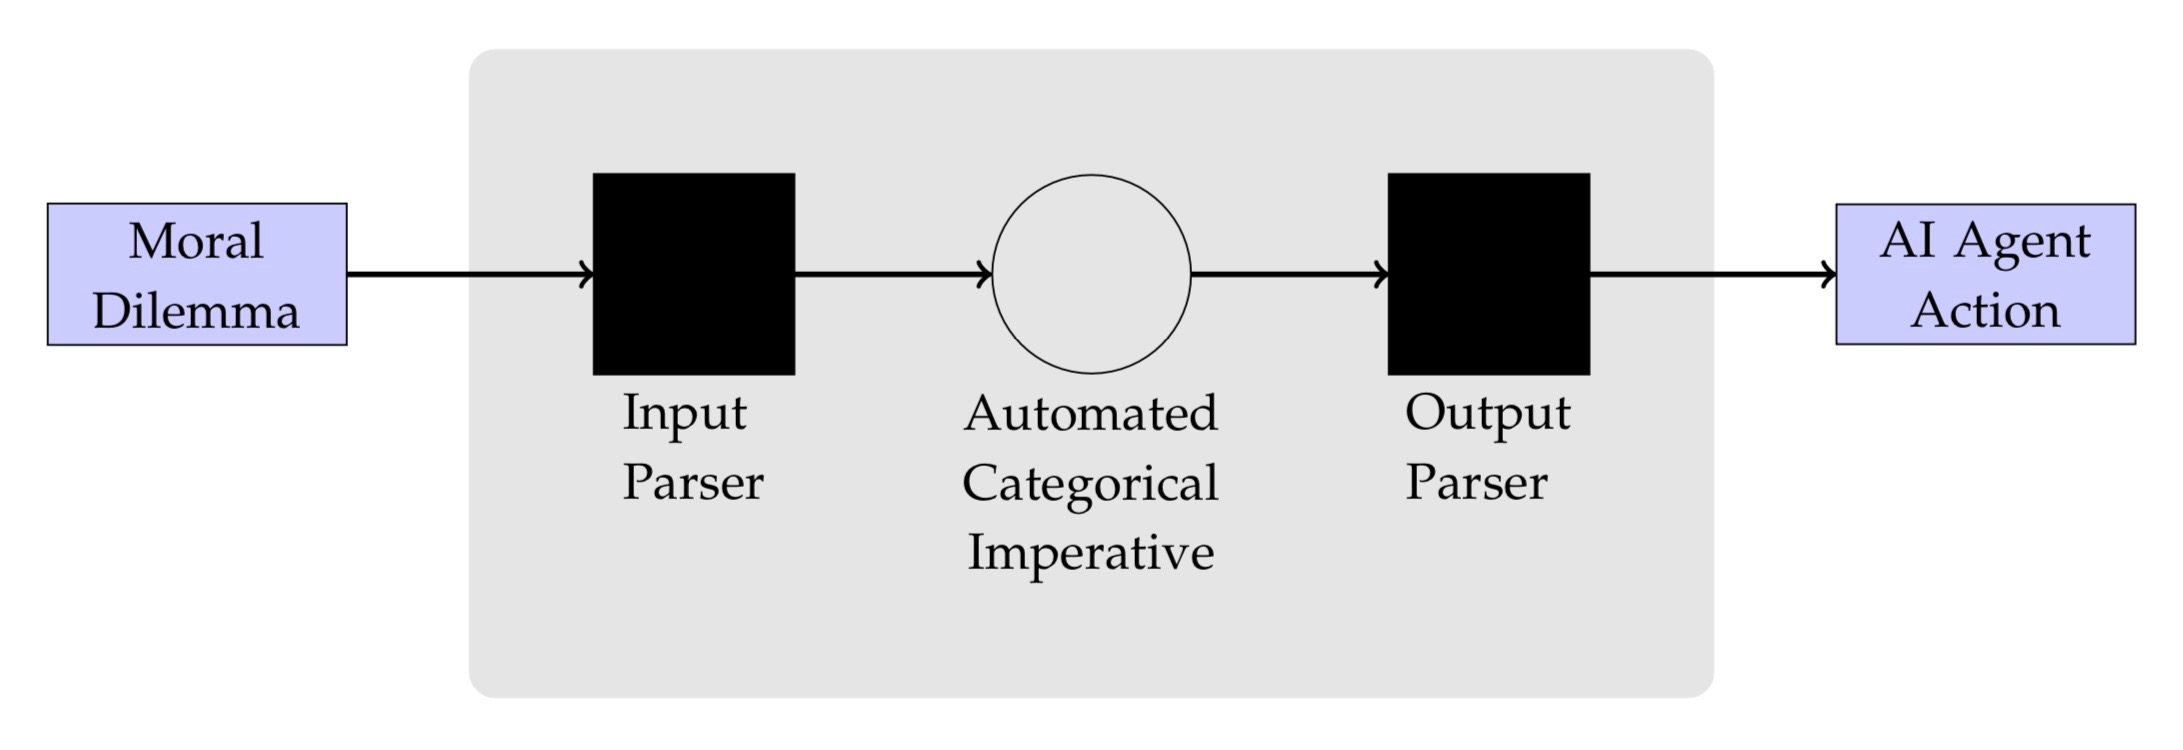
\includegraphics[scale=0.175]{AI_engine.jpeg}
\caption{An example of an ethics engine for artificial intelligence. This ethics engine passes a moral dilemma 
through an input parser, applies the automated categorical imperative test, and finally processes the 
output using an output parser, producing a prescription for action. I contribute the automated categorical 
imperative component.} \label{fig:AIengine}
\end{figure} Figure \ref{fig:AIengine} depicts the workflow of this example ethics engine. In order 
for my system to guide AI using this workflow, future work must develop such input and output parsers.

One of the biggest challenges for an ethics engine is the development of an input parser. An input parser 
for my implementation of automated Kantian ethics must translate a complex real-world situation into a 
circumstances, act, goal triple.
This requires that the input parser determine which circumstances are morally relevant
to a maxim, a controversial judgement. As introduced in Section \ref{whatisamaxim},
there is robust debate on the circumstances that should be considered when formulating a maxim, 
inspired by a common criticism of Kantian ethics called the tailoring objection. Recall that the 
tailoring objection is the worry that arbitrarily specific 
circumstances render any maxim universalizable. For example, consider the maxim ``When my name is Lavanya Singh 
and I am wearing a purple shirt and it is November 26th, I will lie in order to get some easy cash.'' 
Even if this maxim is willed universally, the circumstances are so 
specific that lying will not become the general mechanism for getting easy cash, so the lender will 
believe my lie and the maxim will remain effective. By tailoring the circumstances, any maxim can 
evade universalization.

In Section \ref{whatisamaxim}, I introduced the Kantian response to this criticism, which requires that 
the circumstances included in the formulation
of the maxim be morally relevant. In the example above, my purple shirt and the date have no bearing on 
the moral status of lying. On the other hand, consider the maxim, ``When I am unemployed, I will murder
someone in order to take their job.'' The circumstance ``when I am unemployed'' clearly has some moral
relevance to the murder in question; it speaks to the motivation for the murder. 

While this view has intuitive appeal, it raises the question of how we can determine
which circumstances are morally relevant. O'Neill answers this question
by noting that the Formula of Universal Law is
a ``test of moral worth rather than of outward rightness'' \citep[98]{constofreason}. The FUL is a way 
for an agent to decide how they should behave, not for a third-party to judge their behavior. Ethics is 
a personal process and the FUL is designed to help agents make decisions for themselves. Because agents use 
the FUL to evaluate their own behavior, the test is at its 
best when they make a good faith effort to isolate the \emph{principle} of their action, rather than some
``surface intent'' \citep[87]{constofreason}. The FUL is supposed to determine if an agent's principle of action
is universally consistent, so it is most effective when an agent accurately formulates the principle that
they act on. Circumstances are morally relevant if they reflect the way that the agent is 
thinking about their own action. In the example above, the circumstance of wearing a purple shirt doesn't reflect
the principle of the liar's action. Its inclusion is a disingenous attempt to evade the universalizability
test, but because the FUL is a test of personal integrity, it cannot withstand this kind of mental
gymnastics. 
 
While the above account explains how a well-intentioned human agent can determine 
morally relevant circumstances, the challenge remains open for automated ethics. However an action is turned into a maxim for my system 
to process, whether manually as I did in Chapter \ref{applications} or using an automatic input 
parser, this transformation must be a good-faith attempt to capture the principle of action. 
Such a good-faith attempt to formulate a maxim requires what Kantians call ``practical judgement,'' or
common sense reasoning and factual background \citep{oneilluniversallaws}. Returning to the example above, the fact that being 
unemployed may contribute to one's desire to steal another's job is a consequence of practical
judgement, not just pure reason alone. Automating the formulation of a maxim requires
endowing a machine with common sense. 

Translating everyday situations into appropriate maxims is the bulk of the reasoning that a Kantian 
human being does when making decisions, so it is unsurprising that formulating a maxim 
is one of the biggest obstacles to using my categorical imperative library
in an AI ethics engine. One solution is for a human being to perform the role of the input
parser by supervising the operation of an AI system. When the system stumbles onto
an ethical dilemma, the human could take over, formulate
the right question, and feed it into the categorical imperative library to see what action the categorical 
imperative would prescribe. Alternatively, AI developers can identify expected ethical dilemmas 
that the machine may face in advance and hardcode their own judgements for these dilemmas. 
For proponents of the ``human-in-the-loop'' model of AI ethics, in which
ethical AI requires that humans guide machines, this kind of human involvement may be a feature \citep{loop}.
Both of these solutions imply that the outcome of the universalizability test will depend on how the 
human formulates the maxim; if the human puts garbage into the test, the test will return garbage out.

It is likely that, regardless of the strengths of the human-in-the-loop model, fully automated AI 
will exist. Even if developing this kind of AI is irresponsible,
such developments are likely and will require ethics engines, or risk no consideration of ethics at all.
In such a world, the input parser in my ethics engine would have to be automated.
It is likely that, just as implementations of automated ethics choose 
a particular ethical theory and implement it, different implementations of such an input parser may 
adopt different interpretations of maxim formulation and morally relevant circumstances. 

These interpretations could inspire heuristics to classify circumstances as morally 
relevant. For example, one such attempt could define a moral closeness relation between an act, a 
goal, and circumstances. This heuristic could define morally relevant circumstances as those that 
reach a certain closeness threshhold with the act and the goal. Another possible heuristic could 
define some set of morally important entities, and classify morally relevant circumstances as those
that involve morally important entities. I propose a potential machine-learning based approach which formulates
maxims based on a training set of appropriately formulated maxims in Section \ref{amapossible}. This 
approach mimics how human beings formulate maxims; we use common sense and prior situational, 
factual, and ethical knowledge to isolate our principle of action. Determining morally relevant circumstances, 
either using heuristics or human involvement, is a ripe area for future work.

Once the input has been parsed, either by a human or a machine, into a sentence in my logic, my 
project can evaluate its moral status using my implementation of 
the FUL. Concretely, my project returns a value indicating if the maxim is obligatory, permissible, 
or prohibited. The maxim is prohibited if it fails the universalizability test, permissible if it passes, and obligatory 
if its negation fails the universalizability test. All three of these properties require testing if a 
certain theorem holds or not in my logic, a calculation that I demonstrate in Section \ref{testing}. 
Testing these properties requires that my system have a database of common sense or factual background. 
Different applications of my system may require different factual background (e.g. a self-driving car 
needs to know traffic regulations), so this common sense database will need to be application 
specific. As demonstrated in the examples in Chapter \ref{applications}, my system can produce sophisticated 
judgements with relatively little situational context. Thus, while my automated categorical imperative system
requires some common sense and factual background, Chapter \ref{applications} demonstrates that automating
this common sense is less daunting than it seems.

My system's output could be converted into some actionable, useful response with an output parser, 
and then passed back to the AI system. For example, if the AI system is equipped to evaluate natural 
language prescriptions, the status of the maxim could be parsed into a natural language sentence. The 
input parser, categorical imperative, and output parser together constitute an ``ethics engine'' 
that AI developers could use in a variety of AI systems.

The ethics engine depicted above is a high-level example of one way to use my project to guide artifical intelligence,
with additional work to parse the input and output of my implementation of the categorical imperative.
The kind of automated ethics that I implement could be part of a library that AI developers use to 
give AI the capacity for sophisticated ethical reasoning faithful to philosophical literature. 
This represents an improvement over existing automated ethics, which rarely captures the complexity 
of any ethical theory that philosophers plausibly defend.%
\end{isamarkuptext}\isamarkuptrue%
%
\isadelimdocument
%
\endisadelimdocument
%
\isatagdocument
%
\isamarkupsubsection{Computational Ethics \label{computationalethics}%
}
\isamarkuptrue%
%
\endisatagdocument
{\isafolddocument}%
%
\isadelimdocument
%
\endisadelimdocument
%
\begin{isamarkuptext}%
In addition to guiding AI, automated ethics can also help academic philosophers make philosophical
progress. Just as theorem provers make mathematics more efficient and push mathematicians to think 
precisely about the phenomena they model, computational ethics can help philosophers ask and answer
new philosophical questions. In Section \ref{joking}, I presented one example of the power of computational ethics
by using my system to isolate a necessary and sufficient condition for lying, or knowingly saying
something false, to be wrong. In this section, I share another example of the kind of philosophical 
insight that computational ethics can prompt and analyze the value that this tool can offer to philosophers.\footnote{
I present a final example of computational ethics in Appendix \ref{weirdtests}, where I resolve an ambiguity 
in Korsgaard's argument for the wrongness of false promising using my system \citep{KorsgaardFUL}.} 
Fields from protein folding to game theory are uncovering new insights using computational tools, and computational
ethics harnesses this power to inspire similar progress in philosophy.%
\end{isamarkuptext}\isamarkuptrue%
%
\isadelimdocument
%
\endisadelimdocument
%
\isatagdocument
%
\isamarkupsubsubsection{Example of a Philosophical Insight: Well-Formed Maxims%
}
\isamarkuptrue%
%
\endisatagdocument
{\isafolddocument}%
%
\isadelimdocument
%
\endisadelimdocument
%
\begin{isamarkuptext}%
As presented in Section \ref{formalizingful}, in the process of formalizing
the FUL, I discovered that certain kinds of maxims are badly formed, or inappropriate inputs to the 
universalizability test. The FUL is consistent if it only holds for well-formed maxims,
such that neither the act nor goal are already achieved in the given circumstances. Precisely, 
a circumstance, act, goal tuple (c, a, g) is well-formed if $(\neg (c \longrightarrow a) ) \wedge 
(\neg(c \longrightarrow g))$, or if the circumstances imply neither the act nor the goal. The insight
that the FUL does not apply to badly-formed maxims has philosophical value and serves as evidence 
of the potential of computational ethics. In the next section, I explore this insight using 
Kantian literature. In the following section, I demonstrate the philosophical implications of well-formed
maxims by using this insight to resolve a tension between self-doubt and self-respect. The idea of well-formed
maxims can guide the formulation of maxims and thus may have implications for many parts of Kantian ethics.

\noindent \textbf{Badly-Formed Maxims and Kantian Ethics}

Isabelle gave a logical argument for why the FUL can only hold for well-formed maxims, and I return to Kantian
literature to better understand this idea. In this section, I argue that 
because badly-formed maxims
neither change an agent's behavior nor generate meaningful obligations, they are not the right kinds of 
actions for practical reasoners to make moral judgements about. They cannot be action-guiding and are thus not the kind of problem that 
ethics should be concerned with. Moreover, under the Kantian account of the will, the very act of asking 
if a badly-formed maxim is prohibited generates a contradiction by undermining the will's authority over itself. 

Consider the example badly-formed maxim, ``When eating breakfast, I will eat breakfast in order to 
eat breakfast.'' There is something empty about this maxim because acting on it could never result in 
any action. If I adopt this maxim as a principle to live by,
I decide that, in the circumstances ``eating breakfast'' I will perform the act ``eating breakfast''
for the purpose ``eating breakfast.'' In these circumstances, the act has 
already been performed. Adopting this maxim as a law to live by does not change how I live. If I adopt 
this maxim, then when I am eating breakfast, I eat breakfast, but this statement is already tautologically true. 

Not only does a badly-formed maxim fail to prescribe action, any obligations or prohibitions it 
generates have already been fulfilled or violated. If a badly-formed maxim generates a prohibition, 
then this prohibition is impossible to obey, which is why my original version of the FUL was inconsistent. 
It is impossible to not eat breakfast while eating breakfast, because the circumstances assume that the 
act has happened. On the other hand, if a badly-formed maxim generates an obligation, then the obligation 
will have already been fulfilled. If you are required to eat breakfast while eating breakfast, then you've 
already fulfilled your obligation because the circumstances assume that the act has happened. Thus, 
a badly-formed maxim does not actually guide action because it doesn't generate new obligations or 
prohibitions. 

Because badly-formed maxims can't prescribe or alter action, they are not practically action-guiding and 
thus are not the right kinds of maxims for practical reasoners to evaluate. Insofar as ethics 
is supposed to guide action, badly-formed maxims cannot be part of this project because they
have no bearing on what someone should do. Practical reason is the kind of reason that helps us decide 
what we should do. A practical reasoner asks moral questions not as a mental puzzle or out of curiosity, but 
to decide how to act. A badly-formed maxim is not the kind of maxim that a practical reasoner should consider, because it
will have no bearing on what the agent should do.

Kantians can make an even stronger claim about badly-formed maxims—because maxims are laws that you 
give to yourself, asking if you should will a maxim as you will it undermines your will's law-giving 
ability. The circumstances of a badly-formed maxim assume that the agent has willed the maxim. Under 
the Kantian acount of willing, willing a maxim is equivalent to giving the maxim to yourself as a law. 
When you will a maxim, you commit yourself to the maxim's end. You cannot simultaneously 
commit yourself to a maxim and ask if you should be committing to it. To will the maxim is to adopt it as 
law—so the question, ``should I be willing this?'' is paradoxical. Either you haven't actually made 
the maxim your law (and thus haven't yet committed to it), or you aren't actually asking 
the question (because the decision has already been made). Because a maxim is a law that you give to 
yourself, you cannot question it absent a sufficient reason, such as a change in the circumstances. 
To question a law arbitrarily is to not regard it as a law at all. This kind of questioning amounts to 
questioning the will's authority over itself, but this is impossible.\footnote{Recall from Section \ref{kantianethics} 
that \citet{velleman} presents this argument for the inescapability of practical reason.} The will 
definitionally has authority over itself, for that is what it is to be a will. 

A skeptic may argue that we do often ask ``should I be doing this?'' as we do something. 
To understand this worry, I consider the maxim, 
``When dancing, I should just dance for the sake of dancing.'' While this maxim appears to be badly-formed (the 
circumstance ``dancing'' implies the act and goal of dancing), it is one that practical reasoners 
do consider. I argue that the correct interpretation of this maxim is no longer a badly-formed maxim.

Under one reading of this maxim, ``I should just dance'' is referring to a different act than the 
circumstance ``when dancing.'' The circumstance ``when dancing'' refers 
to rythmically moving your body to music, but ``I should just dance'' refers to dancing without anxiety, 
completely focused on the joy of dancing itself. More precisely, this maxim should read ``When 
dancing, I should abandon my anxiety and focus on dancing for the sake of dancing.'' This maxim when so 
modified is not badly-formed at all—abandoning anxiety and focusing on dancing is an entirely different act 
from moving your body rythmically to music. The circumstances do not entail the act or the goal because 
they refer to different meanings of the word dancing. Any valid reading of this maxim will have the structure above, 
in which the act is actually different from the circumstances. A reasoner cannot accept their will 
as law-giving, or commit themselves to an act, and simultaneously question the act. Either they must be 
questioning a different act or they must have recieved new information to prompt the questioning, 
modifying the circumstances of the original maxim. 

Another related worry concerns maxims that we think are prohibited. Consider the maxim modified to 
read ``When dancing and seeing a child drowning, I should dance for the sake of dancing.'' Clearly this 
maxim is fit for moral evaluation, and we expect a moral theory to prohibit this maxim. The circumstances 
``When dancing and seeing a child drowning'' appear to entail the act of dancing, and the maxim thus 
appears badly-formed. Once again, this maxim is formulated incorrectly. In this case, the question 
that the agent is actually asking themselves is ``should I continue dancing?'' That is the 
maxim that they will adopt or reject. They want to know if they should stop dancing and go help the child. 
Dancing at the current moment and dancing at the next moment are different acts, and the circumstances 
imply the former but not the latter. A badly-formed maxim would have circumstances and act both 
``dancing at moment t,'' but this maxim has circumstances ``dancing at moment t'' and act ``dancing 
at moment t+1.''

\noindent \textbf{Implications for Self-Doubt and Self-Respect}

Above, I defined badly formed maxims, a philosophical concept that I discovered
using computational ethics. In this section, I explore the implications of this concept for the ethical
tension between self-doubt and self-respect to show that computational ethics can result in insights with real 
philosophical weight. The debate between self-doubt and self-respect originates in epistemology, which 
values questioning your beliefs but also rationally requires that you believe that you are not mistaken 
(else you should update your beliefs). I present a parallel tension between self-doubt and self-respect
in ethics, where questioning your judgements is valuable but 
questioning a commitment as you make it is impossible. Ethical self-doubt and self-respect appear 
irresolvably opposed until they are understood through the lens of badly formed maxims. I argue that naive
conceptions of self-doubt are badly formed maxims in disguise. If we reformulate these maxims to be well-formed,
the tension between self-doubt and self-respect dissolves. I sketch the details of this argument in 
the rest of this section. I first introduce the tension between self-doubt and self-respect 
in epistemology, then explain the parallel tension in ethics, and finally present a resolution of this 
tension using badly-formed maxims. I conclude that well-formed maxims form a boundary condition for
the formulation of maxims, so they may resolve many debates in Kantian literature and ethics more generally.

In epistemology, there is a tension between the rational requirement to believe in yourself and the 
value of self-doubt, in moderation. Christensen presents the ``principle of self-respect,'' which requires 
that a rational agent refrain from believing that they have mistaken beliefs \cite[4]{christensen}. For example, I cannot 
rationally believe both that the sky is blue and that I believe that the sky is green. In other words, I cannot 
disapprove of my own credences, since if I do disapprove of them, I should just abandon them. Christensen 
argues that this principle, which he abbreviates to SR, holds because 
a perfectly rational agent can make accurate and confident judgements about what they believe. If this 
is the case, violating SR results in a simple contradiction \cite[8-9]{christensen}. 

While most philosophers accept some version of SR,\footnote{Christensen cites \citet{vanfraassen}, 
\citet{vickers}, and \citet{koons}.}
Roush argues that the principle must be modified in order to account for healthy epistemic 
self-doubt. She argues that, while pathological second-guessing is correctly criticized, we are generally 
imperfect beings, and some sensitivity to our own limitations is a virtue \cite[2]{roushselfhelp}. Even Christensen 
acknowledges that total self-confidence is an epistemic flaw \cite[1]{christensen}. Thus, there is tension between the rational
requirement to respect our authority as believers and the practical reality that we are often wrong. 

This debate between self-respect and self-doubt in epistemology can be extended to ethics. When we 
commit ourselves to acting, we cannot simultaneously doubt the validity of our action, just as we cannot
rationally disapprove of our own beliefs. If human 
behavior is purposive, then the very act of committing implies that one has sufficient reasons for 
committing. These reasons may be flawed, but in making the commitment, the reasoner accepts them—that is 
just what it means to commit oneself to acting. It 
is contradictory to claim that someone commits and questions simultaneously. Either the commitment 
is not real, or the question is not. I will call the principle that one cannot will a maxim and 
simultaneously question if they should will that maxim ``ethical self-respect'' or ESR.

On the other hand, self-doubt is an important part of ethical reasoning. Just as believers are often 
mistaken, so are practical reasoners. An agent who is always sure that they are doing the right thing 
is not thinking deeply enough about their obligations. Some degree of ethical self-doubt is desirable. 
Thus, there is tension between the rational requirement of ESR and the intuitive validity of ethical 
self-doubt (ESD).

I now argue that well-formed maxims can resolve this tension. As in my earlier example, imagine that Sara is dancing at a 
weddding, when, in a moment of angst, she asks herself, ``Should I really be dancing right now?'' 
It seems that she asking if the maxim, ``When dancing at your friend's wedding, dance for the sake 
of dancing'' is a permissible maxim to act on. This maxim is badly-formed: the 
circumstance ``when dancing at a friend's wedding'' implies the act ``dance.'' As I argued above, if 
Sara asks if she should will a badly formed maxim, she is questioning her own will's authority, which
is paradoxical. If expressions of self-doubt are badly-formed maxims, then the tension between ESR
and ESD is natural and unavoidable: debating the permissibility of a badly-formed maxim inherently
involves questioning commitments as we make them, which is impossible. This is the source of the 
tension between ESR and ESD. Those committed to this 
interpretation must abandon one principle or the other, since simultaneous committing and questioning are incompatible.

Because understanding ethical self-doubt as a badly-formed maxim contradicts self-respect, resolving this issue requires a 
different interpretation of ethical self-doubt. Under this interpretation, 
when Sara asks, ``Should I really be dancing right now?'' she wants to know if the maxim that 
resulted in the current moment of dancing was the right thing to will. She is 
asking if she made the right decision in the past, when she decided to dance. The maxim that initiated 
the dancing may be something like ``When at a wedding, dance for the sake of dancing.'' This is the maxim 
that she is currently acting on, not the badly-formed maxim  from above. Under this interpretation, 
there is no tension at all between self-doubt and self-respect. It is perfectly valid for a reasoner 
to doubt their prior moral judgements, just as it is perfectly rational for a believer to doubt their 
past beliefs \cite[3-4]{christensen}. Such doubt does not undermine the reasoner's decision-making 
capacity and is thus perfectly consistent with ethical self-respect. Moreover, this is a much more 
intuitive question to be asking \emph{because} it is a well-formed maxim. Not only is the badly-formed
interpretation of this maxim problematic for ESR, it is also not the kind of question that is useful for a practical
reasoner to ask, as argued above.

Thus, the tension between ESR and ESD arises from a misreading of questions of self-doubt as questions about 
the evaluation of badly-formed maxims. A question of self-doubt cannot refer to a badly-formed maxim and must 
instead refer to a well-formed maxim about the agent's past decision-making. As seen before, cases where 
agents appear to ask themselves about badly-formed maxims are mistaken about the maxim in question, because 
such a question could never yield a useful answer for a practical reasoner. 

By recognizing that the naive version of ethical self-doubt is a badly formed maxim, I realized 
that there is something wrong with its formulation and modified it to resolve the above debate. 
This demonstrates a larger meta-pattern in Kantian reasoning: many debates in Kantian philosophical
literature revolve around incorrectly formulated maxims, which means that the insight about badly
formed maxims may have bearing on these debates. Common misconceptions about Kantian ethics\footnote{For example, critics
of Kantian ethics worry that the maxim, ``When I am a
man, I will marry a man because I want to spend my life with him'' fails the universalizability
test because if all men only married men, sexual reproduction would stop. This argument implies 
that Kantian ethics is homophobic. Kantians often respond by arguing that the correct formulation of 
this maxim is, ``When I love a man, I will marry him because I want to spend my life with him,'' which
is universalizable because if everyone marries who they love, some men will marry women and others will
marry men.} often result from incorrectly formulated maxims, 
and the entire field of applied Kantian ethics is devoted to generating the right kinds of maxims to test. 
Much of the work of a Kantian ethicist is formulating an
appropriate maxim, and badly-formed maxims define one boundary condition for this task. Just as my isolation
of the wrongness of lying in Section \ref{joking} could help guide the formation of morally worthy maxims, 
so can the insight about badly-formed maxims.%
\end{isamarkuptext}\isamarkuptrue%
%
\isadelimdocument
%
\endisadelimdocument
%
\isatagdocument
%
\isamarkupsubsubsection{An Argument For Computational Ethics%
}
\isamarkuptrue%
%
\endisatagdocument
{\isafolddocument}%
%
\isadelimdocument
%
\endisadelimdocument
%
\begin{isamarkuptext}%
The insight above is an example of the kind of philosophical progress that can be 
made using computational tools and serves as evidence for the power of computational ethics. The 
idea that the FUL can only hold for well-formed maxims would have been
incredibly difficult to discover without a computer. I discovered it while formulating the FUL because 
Isabelle's proof-finding tools look for edge cases like badly-formed maxims. Badly-formed maxims are 
interesting precisely because they are the kind of thing that is usually ignored in ordinary philosophical inquiry. 
Philosophers usually assume that we are not discussing badly-formed maxims because, as argued above, 
they are not the kind of thing that is immediately relevant to ethics. Computational tools like Isabelle
require that assumptions like the exclusion of well-formed maxims are made precise, and thus force 
philosophers to understand their arguments in a new way. The philosophical insights about lying in Section
\ref{joking} and about well-formed maxims above demonstrate the contributions
that computational ethics makes: it can quickly check edge cases and it uncovers imprecise, ambiguous,
or implicit assumptions.

In some cases, computational ethics may automate calculations too long and tedious for 
any human philosopher to complete. Insights like the one about well-formed maxims, however, could 
have been discovered by a human being but are much easier to reach with computational tools. I do not 
argue that computational ethics uncovers philosophical insights that humans are always incapable 
of reaching. Computational tools prompt philosophers 
to ask new questions that lead to insights, and can thus serve as another tool in a philosopher's arsenal, like a 
thought experiment or counterexample.

The first benefit of computational ethics is precision, which is the goal of much analytic
philosophy. Thought experiments, arguments, counterexamples, and examples 
illustrate features of a concept in the hope of making the concept itself more precise. Computational 
ethics can help philosophers reach the goal of precision. Representing a philosophical idea in logic 
and implementing it in an interactive theorem prover requires making the idea precise to a degree 
that most philosophical conversation does not necessarily require. For example, when formalizing the notion of a 
maxim, I had to understand its components, define it as a circumstance, act, goal tuple, and identify
coherent and consistent types for each of these entities. This precision is also evident in my examination
of lying and joking in Section \ref{joking}, where I isolate the specific cause of lying's wrongness.
This insight could contribute to the rich philosophical literature on deception, and demonstrates the 
philosophical signifiance of precision. This level of precision is possible 
without computational tools, but computational ethics forces it. Type fuzziness and overloaded definitions 
are all too common in philosophical writing and discussion, but computers disallow this kind of imprecision.

Another benefit of computational ethics is that it makes certain kinds of ethical inquiry, such as 
searching for counterexamples or formal ethics, far less tedious. For example, Nitpick can refute 
an ethical statement in seconds by using brute force to construct a counterexample, something that can require hours
of thought and discussion. I arrived at the insight about badly-formed maxims because Isabelle 
can check edge cases, like that of the badly-formed maxim, far more quickly than a human being. Moreover, 
subfields that use symbolic logic to represent philosophical concepts (e.g. philosophy of language) can 
use interactive theorem provers like Isabelle to complete proofs in a matter of seconds. By automating 
away the tedium, computational ethics can give philosophers the tools to ask new kinds of questions.

Computational ethics is in its infancy. Theorem provers are only now beginning to make headway in 
mathematics \citep{buzzardvideo}, even though theorem provers were first invented in the 1960's \citep{historyofITP}. 
In contrast, the first attempts to use theorem provers to automate deontic logic occurred in the last
few years. The fact that this nascent technology is already helping humans reach non-trivial ethical conclusions 
is reason to, at the very least, entertain the possibility of a future where computational ethics 
becomes as normal for philosophers as using a thought experiment.

To the skeptic, the fact that a theorem prover requires specialized knowledge outside of the field 
of philosophy indicates that the technology is nowhere near ready for universal use in philosophy 
departments. However, history indicates that as computing power increases and computer scientists make 
progress, computational ethics will become more usable. Theorem provers in mathematics began as toys 
incapable of proving that the real number 2 is not equal to the real number 1, but 
moving from basic algebra to Fields medal winning mathematics became possible in a
matter of years \citep{buzzardvideo}. Countless examples from the history of computer science, from the Turing 
Test to AI game playing to protein folding, demonstrate that progress in computer science can make seemingly 
obscure computer programs useful and usable in ways that exceed our expectations.
Programmable computers themselves initially began as unwieldy punch card readers, but their current ubiquity 
need not be stated. If computer scientists and philosophers invest in computational ethics, it could
become as commonplace in philosophy departments as reflective equilibrium. Just as computational tools
have amplified progress in healthcare and drug discovery, computational ethics has the potential to enable
great philosophical progress.%
\end{isamarkuptext}\isamarkuptrue%
%
\isadelimdocument
%
\endisadelimdocument
%
\isatagdocument
%
\isamarkupsubsection{Automating Everyday Practical Reason \label{ordinarypeople}%
}
\isamarkuptrue%
%
\endisatagdocument
{\isafolddocument}%
%
\isadelimdocument
%
\endisadelimdocument
%
\begin{isamarkuptext}%
In Sections \ref{AIethics} and \ref{computationalethics}, I outline how automated ethics can guide
AI and philosophers respectively. This raises a natural question: can automated
ethics guide all human beings, not just academic philosophers, as we navigate the world and face ethical
dilemmas? Some may hope (or worry) that automated ethics could render everyday ethical reasoning obsolete. In 
this section, I argue that while computers should not replace human ethical reasoning entirely,
they can supplement and improve our ethical reasoning. I argue for a kind of human-computer symbiosis
in which computers offer ethical advice, arguments for particular moral judgements, and speed up moral
calculations without subverting human ethical reasoning entirely \citep{licklider}.

Ethics bears weight for everyone, not just for academic philosophers, because it studies the unavoidable question:
how should we live? The ethical question is the only question that 
we answer merely by living. To turn away from ethics is to take a stance on the question of how to 
live (namely, to live unreflectively) and thus to engage in ethics. Every rational being must decide 
how to navigate the world and ethics answers this question. Given that ethics is vital, it seems that if
comptuational tools can help us derive ethical judgements more efficiently, then everyone should engage
in computational ethics. In the most extreme case, we can unthinkingly follow the commands of an 
ethical calculator that dictates how we should live. Maybe computers can answer the unavoidable question for us.

The argument above places the value of ethics solely in its action-guiding potential, and thus fails to take into account the 
importance of practical reason, which, as I argued in Section \ref{kantianethics}, is the source
of freedom itself. We are committed to ethical reflection because of the kind of beings that we are. 
Recall that Korsgaard argues that, as beings occupying minds with a reflective structure, when faced with 
a choice,``it is as if there were something over and above all of your desires, something that is you, and that chooses which desire 
to act on'' \citep[83]{sources}. This choosing is the operation of practical reason, and this reflection
makes us free. We are free because we can choose which reasons to act on. 

If reflection makes us free, then unthinkingly obeying a computer sacrifices our autonomy. Consider 
an Ethics Oracle that can unfailingly tell you the right thing to do in any 
situation.\footnote{This example is inspired by the Pocket Oracle presented in \citet{bok}. Unlike the
Ethics Oracle, Bok's Pocket Oracle perfectly predicts what we \emph{will} do, not what we \emph{should} do.} Someone 
who surrenders themselves to this Oracle unthinkingly follows its prescriptions. 
The reflection involved in the decision to obey each of the Oracle’s prescriptions is limited \citep{bok}. 
This person is not reflecting on the real matters at hand and is 
not making decisions for themselves. They have surrendered their reflective capacity to the Oracle. 
They live a worse life than someone who reflects on their actions; they have less ownership over their 
actions than the reflective person. In a less extreme case, a person may retain control of many of 
their decisions but cede some important or tricky choices to the Ethics Oracle. Because every single 
exercise of practical reason is an exercise of autonomy, this person is still less autonomous than the 
purely reflective person. Even surrendering simple, inconsequential decisions such as which flavor of 
coffee to drink surrenders some piece of our autonomy. Perhaps in trivial cases we can accept that 
tiny sacrifice, but giving over life-changing decisions to the machine sacrifices our 
core freedom. Unreflectively relying on computational ethics surrenders our autonomy to the machine. 

One objection to this emphasis on reflection is the impracticality of making ethical calculations from first principles 
every time we are faced with a decision. This is why we follow the advice of moral mentors, like our 
family or influential philosophers. 
Most people do not reason about ethics during everyday decisions; they rely on some combination of 
prior knowledge and external testimony. For example, my mother taught me to respect myself, so I 
follow her advice. 

What is the difference between following the guidance of a moral educator and
obeying the Ethics Oracle? The best kind of ethical advice prompts reflection, such as an argument 
made in a philosophy paper. Unthinkingly following someone’s advice results in the same loss of 
autonomy as unthinkingly obeying the Ethics Oracle; people who merely obey orders are less autonomous 
than those who think for themselves. This account of moral advice offers a model for human-computer 
symbiotic computational ethics. The computer should serve as a moral guide by providing arguments, just as my mom 
explained why I should always respect myself. Human-computer symbiotic computational
ethics nurtures autonomy when it not only offers prescriptions for action, but also explanations for 
these prescriptions. Because my theorem-prover-based automated ethical system is explainable, it can 
guide action without sacrificing autonomy. It can make an argument for some action, instead of 
merely giving a verdict. Isabelle can list the facts used to show
a partcular action prohibited, and a human being can reflect on whether or not these principles
indeed prohibit the action in question. The computer serves as a collaborator and a tool, but not as an authority, 
so the human being’s reflective capacity and freedom is preserved. 

The above model of human-computer symbiosis demonstrates how computational ethics can augment human
ethical reasoning without replacing it. When deliberating over moral dilemmas, ordinary people can 
turn to computational tools for advice, like an ``Ask an Ethicist'' column. If we appeal to philosophically
faithful computational ethics like that implemented in this thesis, then this advice will synthesize 
decades of philosophical progress and is thus a way to apply philosophers' insights to ordinary life. 
Moreover, just as they do for philosophers, computers can help ordinary people approach ethical questions from a 
different perspective. Even interacting with my system requires the user to consider the action's maxim, 
which includes the circumstances, act, and goal. Making these components of action precise already changes
the user's perspective. Just as computational ethics can serve as a tool for academic philosophers to 
ask new questions and achieve greater precision, it can do the same for all human beings navigating
the world. Moreover, it also offers another way for the general public to access professional philosophy's
insights, and thus carries potential to improve our everyday reasoning.%
\end{isamarkuptext}\isamarkuptrue%
%
\isadelimdocument
%
\endisadelimdocument
%
\isatagdocument
%
\isamarkupsubsection{Theoretical Objections to Automating Kantian Ethics \label{amapossible}%
}
\isamarkuptrue%
%
\endisatagdocument
{\isafolddocument}%
%
\isadelimdocument
%
\endisadelimdocument
%
\begin{isamarkuptext}%
Many philosophers cringe at the idea that a computer could perform ethical reasoning or that the 
categorical imperative could provide an algorithm for moral judgement. For example, Rawls asserts, 
``it is a serious misconception to think of the CI-procedure as an algorithm intended to yield, 
more or less mechanically, a correct judgment. There is no such algorithm, and Kant knows this'' \citep[166]{rawlslectures}. 
Ebels-Duggan also claims, ``no one supposes that the Categorical Imperative provides a mechanical 
algorithm that delivers all by itself a complete account of what we ought to do in any given 
situation'' \citep[174]{ebelsduggan}. However unmechanical ethical reasoning
may seem, these claims are not obvious and require further justification. Philosophers who believe 
that mental activity completely determines moral reasoning must explain why computers can, in theory, 
simulate certain mental processes like arithmetic and language, but cannot perform ethical reasoning. 
Without a soul or God-based account of ethical reasoning, it is not obvious that it is theoretically 
impossible to automate ethical reasoning. After all, computers may eventually learn to simulate human 
mental activity entirely, as shown by progress in brain simulation \citep{brainsimulation}. Skeptics
about automated ethics must explain why ethics is any different from other automated human activity.

The above claims represent the general view that automating ethics is impossible. In the
rest of this section, I explore specific arguments within this view. First, I consider the argument 
that machines cannot have the necessary motivations or attitude towards action to behave morally. Second, 
I consider the difficulty of formulating
an input to the categorical imperative. Third, I consider the strongest objection to automated ethics, 
that moral judgement requires prior ethical knowledge and intuition that machines lack. I argue that 
these objections do not render automated Kantian ethics impossible, but merely difficult. Rawls may be 
correct that there is no simple algorithm for ethical reasoning, but, as
I demonstrate in this thesis, moral judgement using the FUL can be automated using not one
algorithm, but the many algorithms that constitute my system.

\medskip

\noindent \textbf{Machines, Morality, and Motivation}

In \emph{Universal Laws and Ends In Themselves}, O'Neill argues against the existence of an algorithm for
moral behavior. She points out that Kant draws an important distinction between a morally worthy maxim
and a morally worthy action: the latter requires a good will, or a will motivated by duty \citep[345]{oneilluniversallaws}. 
Moral behavior doesn't just require performing
a ``good'' action, but it requires acting on a morally worthy maxim from the motivation of duty, or 
doing the right thing because it is the right thing to do. It is this capacity 
for self-motivation that makes morality binding for rational beings; we must behave morally precisely 
because we have wills, or the ability to be motivated by ends
that we choose. Only rational beings have wills, so only rational beings can have good wills, so only 
rational beings can behave morally. Under this understanding
of moral behavior, it seems unlikely that a computer could behave morally
since a computer does not have motivation in the same way as a human being.\footnote{A parallel argument can also be made for virtue ethics. Virtuous
behavior requires not only a certain action, but also a certain disposition towards the action, so it seems
difficult for AI to truly behave virtuously.}

The idea that a computer cannot behave morally does not preclude the kind 
of automated categorical imperative that I present in this thesis. O'Neill argues that the FUL
serves as a test of morally worthy maxims, and a implementation of an automated categorical imperative can 
identify this kind of maxim. Perhaps a computer cannot act on a morally relevant maxim from the motivation of duty, 
but it certainly can act on this maxim nonetheless. For example, a self-driving car can choose to swerve to hit a tree
to avoid injuring pedestrians in the crosswalk. This action may be one that acts on a morally worthy maxim
\emph{even if} the self-driving car is not motivated by duty. The discpline of machine ethics is
spurred by the recognition that, as automated agents become more powerful, they will need to make
morally consequential decisions. Automated agents may be incapable of moral motivation, but automated agents that mimic
moral behavior are better than agents that ignore morality entirely. AI is navigating a world 
inhabited by human beings, and its decisions impact us. Insofar as AI will operate in human society, 
the behavior of such AI should mimic the behavior of an ethical human being for our sakes, so that we 
can interact with it safely. 

\medskip 

\noindent \textbf{Inputs to the Categorical Imperative}

Another challenge for automated Kantian ethics is that the FUL test requires that
a maxim be given as input. O'Neill notes that the test assumes ``that agents will have certain tentative 
plans, proposals and policies which they can consider, revise or reject or endorse and pursue'' \citep[343]{oneilluniversallaws}.
The FUL evaluates the moral worth of a maxim given as input, where this potential maxim is generated by 
the choices that an agent is faced with. As I argue in Section \ref{AIethics}, determining this potential maxim is a challenge for both human
and automated reasoners. Kant claims that determining an agent's potential maxim is difficult because a maxim is their
personal understanding of their principle of action, so we may never be able 
to know if the morally worthy action has been performed \cite[345]{oneilluniversallaws}. Reasoners are faced with
choices between potential actions and must determine the maxim, or principle, underlying each potential action.
This is equivalent to a ``mapping'' problem: agents are given situations or dilemmas as input and must map
these to maxims.

The challenge of mapping actions to maxims is a limitation of my system, but it is not insurmountable. In Section \ref{AIethics},
I argued that, before my system can be used in practice, it must be paired with an input parser that can
translate choices that an AI system faces into maxims into a logic that my system can
evaluate. This need follows from the difficulty in mapping a potential action
to the maxim of action, whether concerning human action or machine action. As argued in Section \ref{AIethics},  
human-in-the-loop or heuristic-based approaches could resolve this issue. Determining the maxim of 
action is a challenge for Kantian human beings \citep{oneilluniversallaws}, so it is unsurprising that 
it is a major hurdle for automated Kantian agents. Overcoming this hurdle is not impossible, and progress
in automated ethics could address this concern.

\medskip 

\noindent \textbf{Prior Moral Knowledge}

As one of the strongest arguments against a categorical imperative algorithm, O'Neill argues that 
the FUL is not supposed to provide a mechanism for deriving all morally worthy maxims from scratch. She notes
that ``we usually already have learnt or worked out the moral standing of many common maxims of duty,''
and so approach moral deliberation with an ``almanac'' of morally worthy and empty maxims \citep[394]{oneilluniversallaws}. 
Rational agents navigating the world rarely recalculate the moral status of each potential maxim of 
action; instead, we consult our almanac of maxims. This almanac is generated by moral education, 
absorbed social values, and moral advice from people we trust. The categorical imperative is useful 
to verify the rightness or wrongness of a maxim, but is not part of the bulk of human ethical reasoning.

While human beings cannot repeatedly apply the universalizability test to all potential maxims encountered during 
a moral dilemma, computers have the computational power to do so. Human beings are 
equipped with enough prior knowledge or common sense, to have an almanac of morally worthy maxims,
but we have limited computational power. Computers, on the other hand, are comparatively
much more capable of computation and thus can repeatedly recompute the results of the categorical
imperative test. They do not come equipped with an almanac of maxims, but can simply recompute this
almanac every time they need to make a decision. Human beings use common sense to make up for their computational
limitations, and automated moral agents can use computational power to reduce the need for common sense.

Daniela Tafani takes O'Neill's argument one step further by arguing that this ``alamnac'' of maxims already 
includes the moral status of the maxims in questions; human beings already
know which maxims are morally worthy and which are morally lacking. The categorical imperative test
merely reminds us, in moments of weakness, when we are tempted to make an exception to the moral law for 
our own convenience or pleasure, that the moral law has no exceptions \citep[9]{tafani}. Thus, she claims
that ``the Kantian test is therefore as useless for machines as it is for anyone who does
not already know what to do'' \citep[8]{tafani}.\footnote{Translated from Italian to English using Google Translate.} 
Understanding the categorical imperative test as a reminder
instead of a derivation tool also explains the response to the tailoring objection presented in Section \ref{AIethics}, that the FUL cannot 
handle bad-faith attempts to generate false positives or negatives. The test only returns the right 
result when an agent sincerely attempts to represent their maxim of action, not when an adversary attempts
 to ``trick'' the categorical imperative because such tricks will fall outside the scope of our moral 
almanacs.%
\end{isamarkuptext}\isamarkuptrue%
%
\begin{figure}
\centering
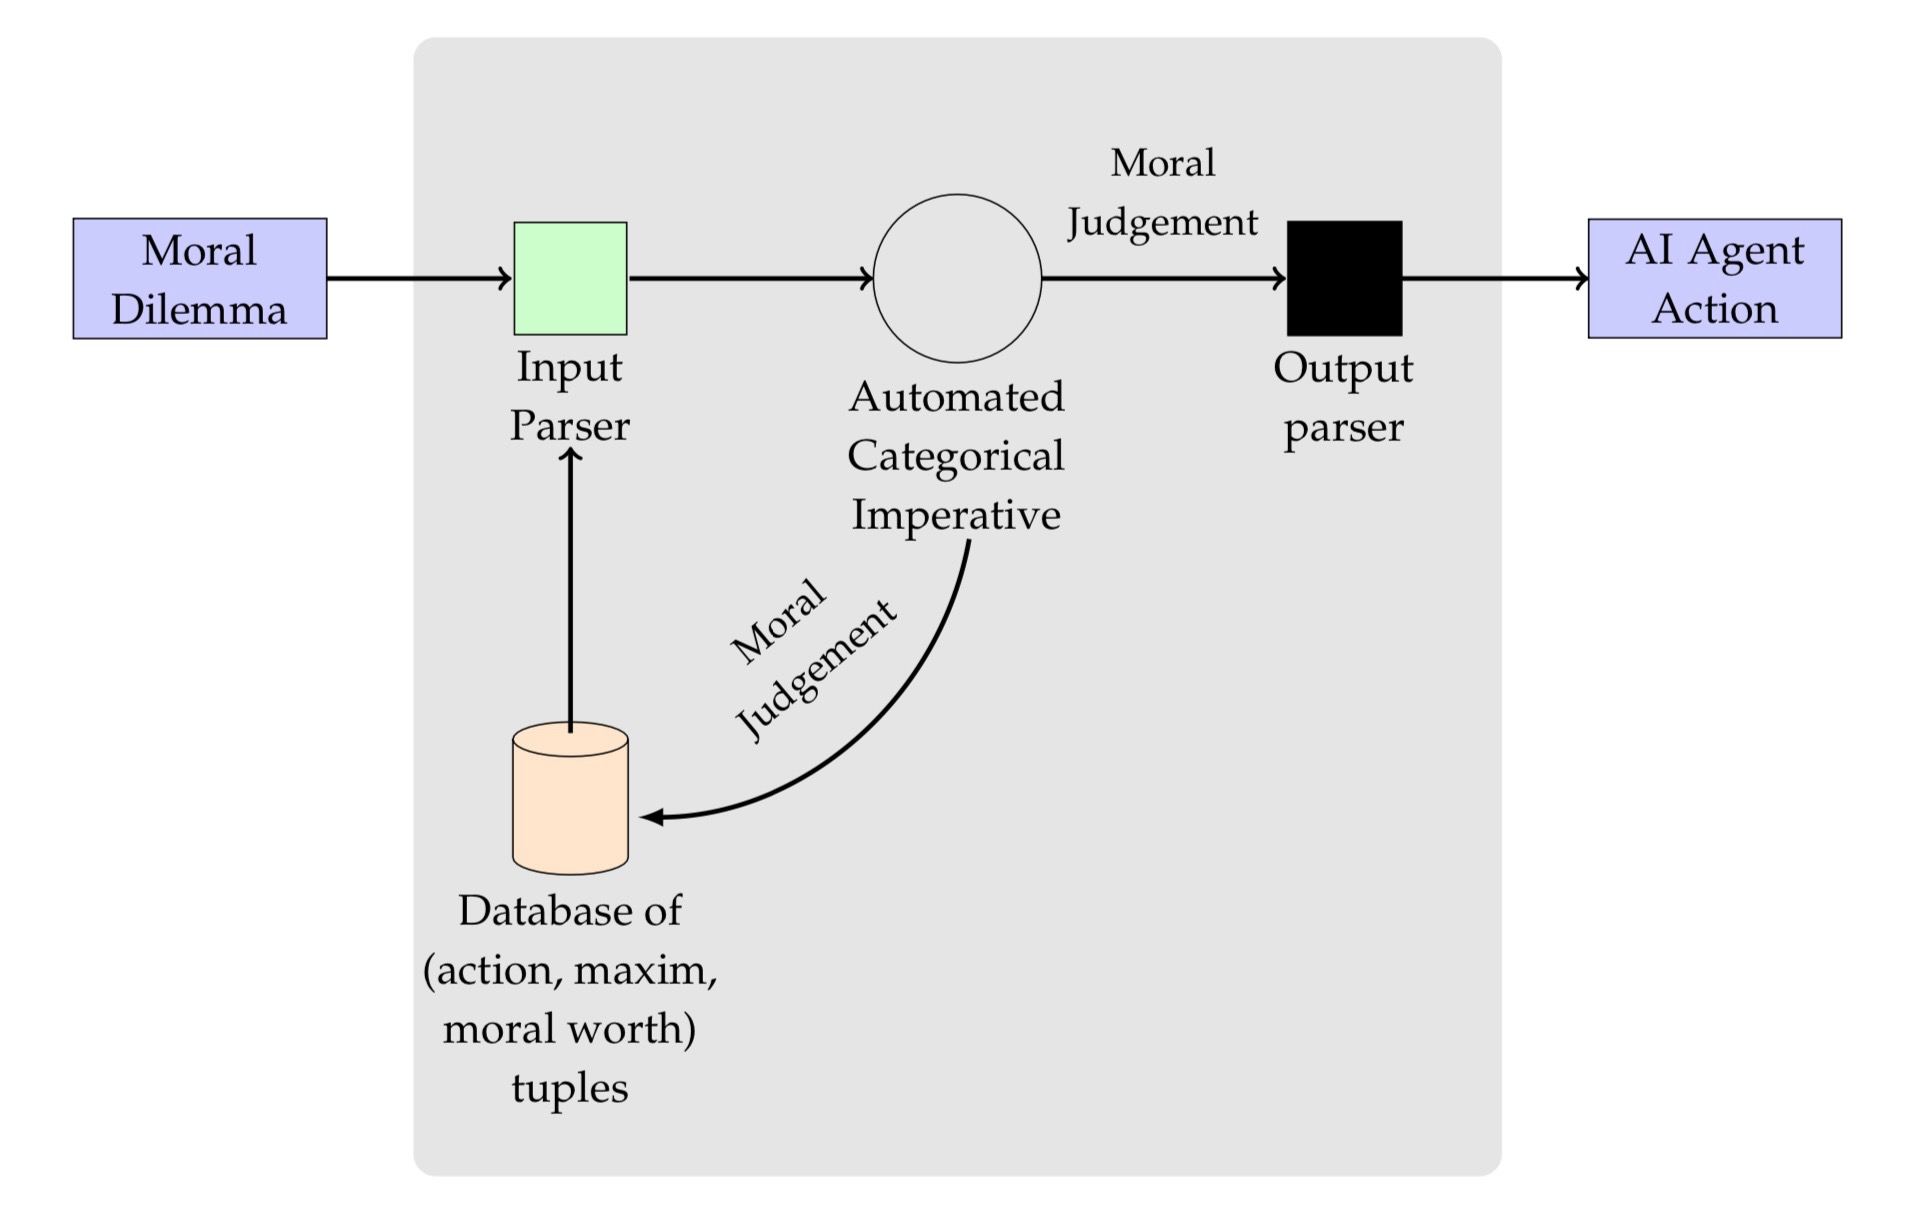
\includegraphics[scale=0.19]{inputparser.jpeg}
\caption{A refined version of Figure \ref{fig:AIengine} in which the input parser learns from a database
of action-maxim mappings, which is in turn fed the output of my automated categorical imperative. } \label{fig:inputparser}
\end{figure}
%
\begin{isamarkuptext}%
Under Tafani's and O'Neill's understandings of the categorical imperative, not only is automated moral reasoning
possible, but the challenge of creating an input parser or automatically formulating a maxim becomes 
easier as well. 
If the categorical imperative test is only useful to those who have some prior moral knowledge, then prior moral
knowledge can and should be used to create an input parser. Specifically, a machine learning-based approach
could learn action-maxim mappings from a database of such mappings compiled by a human being. Moreover, 
the human being could assign each maxim in the database a rightness or wrongness score. My implementation
of the automated categorical imperative would then simply check the work of this machine learning algorithm and transform
a fuzzy prediction into a provable, rigorous moral judgement. This rigorous moral judgement
could in turn be fed into the database of maxims to make the input parser smarter. One example of 
this kind of system is shown in Figure \ref{fig:inputparser}. The combination of 
prior knowledge of some maxims' moral worth and the ability of a computer to constantly perform the
universalizability test could not only match human ethical reasoning but could perhaps surpass it
by double-checking the moral intuitions that we take for granted. A computer with no common sense or prior knowledge
may be unable to reason using the categorical imperative, but one equipped with some prior knowledge
of maxims and their moral worth may even be able to reason about morality better than human beings can.%
\end{isamarkuptext}\isamarkuptrue%
%
\isadelimdocument
%
\endisadelimdocument
%
\isatagdocument
%
\isamarkupsubsection{Related Work \label{relatedwork}%
}
\isamarkuptrue%
%
\endisatagdocument
{\isafolddocument}%
%
\isadelimdocument
%
\endisadelimdocument
%
\begin{isamarkuptext}%
In 1685, Leibniz dreamed of a calculator that could resolve philosophical and theological 
disputes \citep{leibniz}. At the time, the logical and computational resources necessary to make his 
dream a reality did not exist. Today, automated ethics is a growing field, spurred in part by the 
need for ethically intelligent AI. Tolmeijer et al. surveyed the state of the field of 
machine ethics \citep{mesurvey} and characterized implementations in automated ethics by (1) the choice 
of ethical theory, (2) implementation design decisions (e.g. logic programming), and (3) implementation 
details (e.g. choice of logic). 

Automated ethics falls into two branches: top-down and bottom-up ethics. Top-down automated ethics begins 
with an ethical theory, whereas bottom-up automated ethics learns ethical judgements from prior 
judgements. One example of bottom-up automated ethics is Delphi, which uses deep learning to make 
ethical judgements based on a dataset of human judgements \citep{delphi}. While Delphi displays great 
flexibility, it often produces contradictory judgements, such as claiming that taxing exploitative 
profitable companies is good, but burdening successful companies with high tax rates is bad \citep{verge}. 
Because Delphi draws on error-prone human judgements instead of philosophical literature, it makes 
the same judgement errors that humans make. Moreover, because Delphi uses a bottom-up approach, 
there is no explicit ethical theory explaining its judgements, so analytically arguing for or 
against its conclusions is impossible. Top-down approaches, on the other hand, must be explicit about 
the underlying ethical theories, and are thus more explainable. 

In this paper, I use a top-down approach to formalize Kantian ethics. There is a long line of work 
automating other ethical theories, like consequentialism \citep{util2, util1} or particularism 
\citep{particularism1, particularism2}. I choose to implement Kantian ethics because, as argued in 
Section \ref{whykant}, it is the most formal and least data-intensive of the three major ethical 
traditions. Kantian ethics is a deontological, or rule based ethic, and there is prior work 
implementing other deontological theories \citep{deon1, deon2, dde}. 

Kantian ethics specifically appears to be an intuitive candidate for formalization and implementation 
and there has been both theoretical and practical work on automating Kantian ethics \citep{powers, lin}. 
In 2006, Powers argued that implementing Kantian ethics presented technical challenges, 
such as automation of a non-monotonic logic, and philosophical challenges, like a definition of the 
categorical imperative \citep{powers}. I address the former through my use of Dyadic Deontic Logic, which allows 
obligations to be retracted as context changes, and the latter through my use of the practical 
contradiction interpretation. There has also been prior work in formalizing Kantian metaphysics 
using I/O logic \citep{io}. Deontic logic, which has been implemented in Isabelle/HOL, is itself inspired 
by Kant's ``ought implies can'' principle, but it does not include a robust formalization of the entire 
categorical imperative \citep{cresswell}.

Kroy presented a formalization of the first two formulations of the categorical imperative, but wrote 
before the computational tools existed to automate such a formalization \citep{kroy}. I implement his formalization of the FUL to compare it to my system. 
Lindner and Bentzen presented one of the first implementations of a formalization of 
Kant's second formulation of the categorical imperative \citep{BL}. They present their goal as ``not to get 
close to a correct interpretation of Kant, but to show that our interpretation of Kant’s ideas can 
contribute to the development of machine ethics.'' My work builds on theirs by formalizing the 
first formulation of the categorical imperative as faithfully as possible. Staying faithful to 
philosophical literature makes my system capable of making robust and reliable judgements. 

The implementation of this paper was inspired by and builds on Benzmüller, Parent, and Farjami's 
foundational work with the LogiKEy framework for machine ethics, which includes their implementation 
of DDL in Isabelle \citep{logikey, BFP}. The LogiKEy project has been used to study metaphysics 
\citep{godel, metaphysics1}, law \citep{constitution}, and ethics \citep{gewirth}, but not 
Kant's categorical imperative.%
\end{isamarkuptext}\isamarkuptrue%
%
\isadelimdocument
%
\endisadelimdocument
%
\isatagdocument
%
\isamarkupsubsection{Conclusion%
}
\isamarkuptrue%
%
\endisatagdocument
{\isafolddocument}%
%
\isadelimdocument
%
\endisadelimdocument
%
\begin{isamarkuptext}%
In this thesis, I present a proof-of-concept implementation of automated Kantian ethics. My system
takes as input a potential action, appropriately represented, and can prove that it is obligated, 
prohibited or permissible. I represent Kant's Formula of Universal Law in a deontic logic and 
implement this logic in the Isabelle/HOL interactive theorem prover, which can automatically prove or 
refute theorems in my custom logic. I also contribute a testing framework that demonstrates that
my implementation of Kantian ethics is more faithful to philosophical literature than two other 
potential implementations. My completed system can, when given appropriate factual background, make
philosophically mature judgements about complex moral dilemmas. This work is one step towards building 
morally sophisticated artifical intelligence.

The idea of fully automated artificial intelligence navigating the world without human supervision
may be terrifying, but progress in AI indicates that such a future is likely closer than we think. 
Philosophers, regulators, and computer scientists are sounding the alarm about the dangers of developing
this kind of AI. Insofar as developers will continue to ignore these warnings and develop increasingly 
independent AI, there is a dire need to program such AI with some notion of ethics. If AI is navigating
human society, then it is making ethically-tinged decisions at all times. Ethics is inescapable; 
if AI developers and computer scientists ignore it, then they will be building machines that make decisions
based on some set of unknown, implicit ethical values. Countless examples, from the Allegheny Family Screening Tool
that is biased against poor families to search algorithms that associate black-sounding names
with crime, demonstrate that such implicit ethics usually codifies the biases, prejudices, and moral
failings of the society in which it is developed \citep{eubanks, sweeney}. AI will inevitably make judgements on moral dilemmas, 
and automated ethics is necessary to make these judgements morally correct. 

Given that the discpline of philosophy has spent centuries debating such judgements and their theoretical 
underpinnings, such AI will be most trustworthy, nuanced, consistent, and mature when it is faithful to 
philosophical literature. In order to develop high-quality automated ethics, computer scientists and 
philosophers must work together. Neither discipline alone can address the pressing need for ethical AI. 
This thesis is an experiment in marrying philosophy and computer science 
to create automated ethics that is both technically and philosophically advanced. 

This work is an early proof-of-concept. It demonstrates the potential of top-down, logic programming 
approaches to automated ethics and shows that it is possible to faithfully automate an ethical theory as
complex as Kantian ethics. There are open questions that must be resolved before a system like this 
could be used in practice, but this project demonstrates that these questions are within closer reach
than they may seem. Automated ethics does not need to limit itself to simple, flattened versions of 
ethical theories. With technical and philosophical progress, faithful automated ethics is possible.
Growing public consciousness about the dangers of unregulated AI is creating momentum in machine ethics; 
work like Delphi demonstrates that the time is ripe to create usable, reliable automated ethics. This 
thesis is one step towards building computers that can think ethically in the richest sense of the word.%
\end{isamarkuptext}\isamarkuptrue%
%
\isadelimtheory
%
\endisadelimtheory
%
\isatagtheory
%
\endisatagtheory
{\isafoldtheory}%
%
\isadelimtheory
%
\endisadelimtheory
%
\end{isabellebody}%
\endinput
%:%file=~/Desktop/cs91r/paper/thesis_5_discussion.thy%:%
%:%24=6%:%
%:%36=8%:%
%:%37=9%:%
%:%38=10%:%
%:%39=11%:%
%:%40=12%:%
%:%41=13%:%
%:%42=14%:%
%:%43=15%:%
%:%44=16%:%
%:%45=17%:%
%:%46=18%:%
%:%47=19%:%
%:%48=20%:%
%:%49=21%:%
%:%50=22%:%
%:%51=23%:%
%:%52=24%:%
%:%61=26%:%
%:%73=27%:%
%:%74=28%:%
%:%75=29%:%
%:%76=30%:%
%:%77=31%:%
%:%78=32%:%
%:%79=33%:%
%:%80=34%:%
%:%81=35%:%
%:%82=36%:%
%:%83=37%:%
%:%84=38%:%
%:%85=39%:%
%:%86=40%:%
%:%87=41%:%
%:%88=42%:%
%:%89=43%:%
%:%90=44%:%
%:%91=45%:%
%:%92=46%:%
%:%93=47%:%
%:%94=48%:%
%:%95=49%:%
%:%96=50%:%
%:%97=51%:%
%:%98=52%:%
%:%99=53%:%
%:%100=54%:%
%:%101=55%:%
%:%102=56%:%
%:%103=57%:%
%:%104=58%:%
%:%105=59%:%
%:%106=60%:%
%:%107=61%:%
%:%108=62%:%
%:%109=63%:%
%:%110=64%:%
%:%111=65%:%
%:%112=66%:%
%:%113=67%:%
%:%114=68%:%
%:%115=69%:%
%:%116=70%:%
%:%117=71%:%
%:%118=72%:%
%:%119=73%:%
%:%120=74%:%
%:%121=75%:%
%:%122=76%:%
%:%123=77%:%
%:%124=78%:%
%:%125=79%:%
%:%126=80%:%
%:%127=81%:%
%:%128=82%:%
%:%129=83%:%
%:%130=84%:%
%:%131=85%:%
%:%132=86%:%
%:%133=87%:%
%:%134=88%:%
%:%135=89%:%
%:%136=90%:%
%:%137=91%:%
%:%138=92%:%
%:%139=93%:%
%:%140=94%:%
%:%141=95%:%
%:%142=96%:%
%:%143=97%:%
%:%144=98%:%
%:%145=99%:%
%:%146=100%:%
%:%147=101%:%
%:%148=102%:%
%:%149=103%:%
%:%150=104%:%
%:%151=105%:%
%:%152=106%:%
%:%153=107%:%
%:%154=108%:%
%:%155=109%:%
%:%156=110%:%
%:%157=111%:%
%:%158=112%:%
%:%159=113%:%
%:%160=114%:%
%:%161=115%:%
%:%162=116%:%
%:%163=117%:%
%:%164=118%:%
%:%165=119%:%
%:%166=120%:%
%:%167=121%:%
%:%168=122%:%
%:%169=123%:%
%:%170=124%:%
%:%171=125%:%
%:%172=126%:%
%:%173=127%:%
%:%174=128%:%
%:%175=129%:%
%:%176=130%:%
%:%177=131%:%
%:%178=132%:%
%:%179=133%:%
%:%180=134%:%
%:%181=135%:%
%:%182=136%:%
%:%183=137%:%
%:%184=138%:%
%:%185=139%:%
%:%186=140%:%
%:%187=141%:%
%:%188=142%:%
%:%189=143%:%
%:%190=144%:%
%:%191=145%:%
%:%192=146%:%
%:%193=147%:%
%:%194=148%:%
%:%203=150%:%
%:%215=152%:%
%:%216=153%:%
%:%217=154%:%
%:%218=155%:%
%:%219=156%:%
%:%220=157%:%
%:%221=158%:%
%:%222=159%:%
%:%223=160%:%
%:%224=161%:%
%:%225=162%:%
%:%234=164%:%
%:%246=166%:%
%:%247=167%:%
%:%248=168%:%
%:%249=169%:%
%:%250=170%:%
%:%251=171%:%
%:%252=172%:%
%:%253=173%:%
%:%254=174%:%
%:%255=175%:%
%:%256=176%:%
%:%257=177%:%
%:%258=178%:%
%:%259=179%:%
%:%260=180%:%
%:%261=181%:%
%:%262=182%:%
%:%263=183%:%
%:%264=184%:%
%:%265=185%:%
%:%266=186%:%
%:%267=187%:%
%:%268=188%:%
%:%269=189%:%
%:%270=190%:%
%:%271=191%:%
%:%272=192%:%
%:%273=193%:%
%:%274=194%:%
%:%275=195%:%
%:%276=196%:%
%:%277=197%:%
%:%278=198%:%
%:%279=199%:%
%:%280=200%:%
%:%281=201%:%
%:%282=202%:%
%:%283=203%:%
%:%284=204%:%
%:%285=205%:%
%:%286=206%:%
%:%287=207%:%
%:%288=208%:%
%:%289=209%:%
%:%290=210%:%
%:%291=211%:%
%:%292=212%:%
%:%293=213%:%
%:%294=214%:%
%:%295=215%:%
%:%296=216%:%
%:%297=217%:%
%:%298=218%:%
%:%299=219%:%
%:%300=220%:%
%:%301=221%:%
%:%302=222%:%
%:%303=223%:%
%:%304=224%:%
%:%305=225%:%
%:%306=226%:%
%:%307=227%:%
%:%308=228%:%
%:%309=229%:%
%:%310=230%:%
%:%311=231%:%
%:%312=232%:%
%:%313=233%:%
%:%314=234%:%
%:%315=235%:%
%:%316=236%:%
%:%317=237%:%
%:%318=238%:%
%:%319=239%:%
%:%320=240%:%
%:%321=241%:%
%:%322=242%:%
%:%323=243%:%
%:%324=244%:%
%:%325=245%:%
%:%326=246%:%
%:%327=247%:%
%:%328=248%:%
%:%329=249%:%
%:%330=250%:%
%:%331=251%:%
%:%332=252%:%
%:%333=253%:%
%:%334=254%:%
%:%335=255%:%
%:%336=256%:%
%:%337=257%:%
%:%338=258%:%
%:%339=259%:%
%:%340=260%:%
%:%341=261%:%
%:%342=262%:%
%:%343=263%:%
%:%344=264%:%
%:%345=265%:%
%:%346=266%:%
%:%347=267%:%
%:%348=268%:%
%:%349=269%:%
%:%350=270%:%
%:%351=271%:%
%:%352=272%:%
%:%353=273%:%
%:%354=274%:%
%:%355=275%:%
%:%356=276%:%
%:%357=277%:%
%:%358=278%:%
%:%359=279%:%
%:%360=280%:%
%:%361=281%:%
%:%362=282%:%
%:%363=283%:%
%:%364=284%:%
%:%365=285%:%
%:%366=286%:%
%:%367=287%:%
%:%368=288%:%
%:%369=289%:%
%:%370=290%:%
%:%371=291%:%
%:%372=292%:%
%:%373=293%:%
%:%374=294%:%
%:%375=295%:%
%:%376=296%:%
%:%377=297%:%
%:%378=298%:%
%:%379=299%:%
%:%380=300%:%
%:%381=301%:%
%:%382=302%:%
%:%383=303%:%
%:%384=304%:%
%:%385=305%:%
%:%386=306%:%
%:%387=307%:%
%:%388=308%:%
%:%389=309%:%
%:%390=310%:%
%:%391=311%:%
%:%392=312%:%
%:%393=313%:%
%:%394=314%:%
%:%395=315%:%
%:%396=316%:%
%:%397=317%:%
%:%398=318%:%
%:%399=319%:%
%:%400=320%:%
%:%401=321%:%
%:%402=322%:%
%:%403=323%:%
%:%404=324%:%
%:%405=325%:%
%:%406=326%:%
%:%407=327%:%
%:%408=328%:%
%:%409=329%:%
%:%410=330%:%
%:%411=331%:%
%:%412=332%:%
%:%413=333%:%
%:%414=334%:%
%:%415=335%:%
%:%416=336%:%
%:%417=337%:%
%:%418=338%:%
%:%419=339%:%
%:%420=340%:%
%:%421=341%:%
%:%422=342%:%
%:%423=343%:%
%:%424=344%:%
%:%425=345%:%
%:%426=346%:%
%:%427=347%:%
%:%428=348%:%
%:%429=349%:%
%:%430=350%:%
%:%431=351%:%
%:%432=352%:%
%:%433=353%:%
%:%434=354%:%
%:%435=355%:%
%:%436=356%:%
%:%437=357%:%
%:%438=358%:%
%:%439=359%:%
%:%440=360%:%
%:%449=363%:%
%:%461=365%:%
%:%462=366%:%
%:%463=367%:%
%:%464=368%:%
%:%465=369%:%
%:%466=370%:%
%:%467=371%:%
%:%468=372%:%
%:%469=373%:%
%:%470=374%:%
%:%471=375%:%
%:%472=376%:%
%:%473=377%:%
%:%474=378%:%
%:%475=379%:%
%:%476=380%:%
%:%477=381%:%
%:%478=382%:%
%:%479=383%:%
%:%480=384%:%
%:%481=385%:%
%:%482=386%:%
%:%483=387%:%
%:%484=388%:%
%:%485=389%:%
%:%486=390%:%
%:%487=391%:%
%:%488=392%:%
%:%489=393%:%
%:%490=394%:%
%:%491=395%:%
%:%492=396%:%
%:%493=397%:%
%:%494=398%:%
%:%495=399%:%
%:%496=400%:%
%:%497=401%:%
%:%498=402%:%
%:%499=403%:%
%:%500=404%:%
%:%501=405%:%
%:%502=406%:%
%:%503=407%:%
%:%504=408%:%
%:%505=409%:%
%:%506=410%:%
%:%507=411%:%
%:%508=412%:%
%:%509=413%:%
%:%510=414%:%
%:%511=415%:%
%:%512=416%:%
%:%513=417%:%
%:%514=418%:%
%:%515=419%:%
%:%516=420%:%
%:%517=421%:%
%:%518=422%:%
%:%519=423%:%
%:%520=424%:%
%:%521=425%:%
%:%522=426%:%
%:%523=427%:%
%:%524=428%:%
%:%525=429%:%
%:%526=430%:%
%:%535=432%:%
%:%547=434%:%
%:%548=435%:%
%:%549=436%:%
%:%550=437%:%
%:%551=438%:%
%:%552=439%:%
%:%553=440%:%
%:%554=441%:%
%:%555=442%:%
%:%556=443%:%
%:%557=444%:%
%:%558=445%:%
%:%559=446%:%
%:%560=447%:%
%:%561=448%:%
%:%562=449%:%
%:%563=450%:%
%:%564=451%:%
%:%565=452%:%
%:%566=453%:%
%:%567=454%:%
%:%568=455%:%
%:%569=456%:%
%:%570=457%:%
%:%571=458%:%
%:%572=459%:%
%:%573=460%:%
%:%574=461%:%
%:%575=462%:%
%:%576=463%:%
%:%577=464%:%
%:%578=465%:%
%:%579=466%:%
%:%580=467%:%
%:%581=468%:%
%:%582=469%:%
%:%583=470%:%
%:%584=471%:%
%:%585=472%:%
%:%586=473%:%
%:%587=474%:%
%:%588=475%:%
%:%589=476%:%
%:%590=477%:%
%:%591=478%:%
%:%592=479%:%
%:%593=480%:%
%:%594=481%:%
%:%595=482%:%
%:%596=483%:%
%:%597=484%:%
%:%598=485%:%
%:%599=486%:%
%:%600=487%:%
%:%601=488%:%
%:%602=489%:%
%:%603=490%:%
%:%604=491%:%
%:%605=492%:%
%:%606=493%:%
%:%607=494%:%
%:%608=495%:%
%:%609=496%:%
%:%610=497%:%
%:%611=498%:%
%:%612=499%:%
%:%613=500%:%
%:%614=501%:%
%:%615=502%:%
%:%616=503%:%
%:%617=504%:%
%:%618=505%:%
%:%619=506%:%
%:%620=507%:%
%:%621=508%:%
%:%622=509%:%
%:%623=510%:%
%:%632=513%:%
%:%644=516%:%
%:%645=517%:%
%:%646=518%:%
%:%647=519%:%
%:%648=520%:%
%:%649=521%:%
%:%650=522%:%
%:%651=523%:%
%:%652=524%:%
%:%653=525%:%
%:%654=526%:%
%:%655=527%:%
%:%656=528%:%
%:%657=529%:%
%:%658=530%:%
%:%659=531%:%
%:%660=532%:%
%:%661=533%:%
%:%662=534%:%
%:%663=535%:%
%:%664=536%:%
%:%665=537%:%
%:%666=538%:%
%:%667=539%:%
%:%668=540%:%
%:%669=541%:%
%:%670=542%:%
%:%671=543%:%
%:%672=544%:%
%:%673=545%:%
%:%674=546%:%
%:%675=547%:%
%:%676=548%:%
%:%677=549%:%
%:%678=550%:%
%:%679=551%:%
%:%680=552%:%
%:%681=553%:%
%:%682=554%:%
%:%683=555%:%
%:%684=556%:%
%:%685=557%:%
%:%686=558%:%
%:%687=559%:%
%:%688=560%:%
%:%689=561%:%
%:%690=562%:%
%:%691=563%:%
%:%692=564%:%
%:%693=565%:%
%:%694=566%:%
%:%695=567%:%
%:%696=568%:%
%:%697=569%:%
%:%698=570%:%
%:%699=571%:%
%:%700=572%:%
%:%701=573%:%
%:%702=574%:%
%:%703=575%:%
%:%704=576%:%
%:%705=577%:%
%:%706=578%:%
%:%707=579%:%
%:%708=580%:%
%:%709=581%:%
%:%710=582%:%
%:%711=583%:%
%:%712=584%:%
%:%713=585%:%
%:%714=586%:%
%:%715=587%:%
%:%716=588%:%
%:%717=589%:%
%:%718=590%:%
%:%719=591%:%
%:%720=592%:%
%:%721=593%:%
%:%722=594%:%
%:%723=595%:%
%:%724=596%:%
%:%725=597%:%
%:%726=598%:%
%:%727=599%:%
%:%728=600%:%
%:%729=601%:%
%:%730=602%:%
%:%731=603%:%
%:%732=604%:%
%:%733=605%:%
%:%734=606%:%
%:%735=607%:%
%:%736=608%:%
%:%737=609%:%
%:%738=610%:%
%:%739=611%:%
%:%740=612%:%
%:%741=613%:%
%:%742=614%:%
%:%743=615%:%
%:%744=616%:%
%:%745=617%:%
%:%746=618%:%
%:%747=619%:%
%:%748=620%:%
%:%749=621%:%
%:%750=622%:%
%:%751=623%:%
%:%752=624%:%
%:%753=625%:%
%:%754=626%:%
%:%755=627%:%
%:%756=628%:%
%:%757=629%:%
%:%758=630%:%
%:%759=631%:%
%:%760=632%:%
%:%761=633%:%
%:%762=634%:%
%:%763=635%:%
%:%766=637%:%
%:%767=638%:%
%:%768=639%:%
%:%769=640%:%
%:%770=641%:%
%:%771=642%:%
%:%774=643%:%
%:%775=644%:%
%:%776=645%:%
%:%777=646%:%
%:%778=647%:%
%:%779=648%:%
%:%780=649%:%
%:%781=650%:%
%:%782=651%:%
%:%783=652%:%
%:%784=653%:%
%:%785=654%:%
%:%786=655%:%
%:%787=656%:%
%:%788=657%:%
%:%789=658%:%
%:%798=662%:%
%:%810=664%:%
%:%811=665%:%
%:%812=666%:%
%:%813=667%:%
%:%814=668%:%
%:%815=669%:%
%:%816=670%:%
%:%817=671%:%
%:%818=672%:%
%:%819=673%:%
%:%820=674%:%
%:%821=675%:%
%:%822=676%:%
%:%823=677%:%
%:%824=678%:%
%:%825=679%:%
%:%826=680%:%
%:%827=681%:%
%:%828=682%:%
%:%829=683%:%
%:%830=684%:%
%:%831=685%:%
%:%832=686%:%
%:%833=687%:%
%:%834=688%:%
%:%835=689%:%
%:%836=690%:%
%:%837=691%:%
%:%838=692%:%
%:%839=693%:%
%:%840=694%:%
%:%841=695%:%
%:%842=696%:%
%:%843=697%:%
%:%844=698%:%
%:%845=699%:%
%:%846=700%:%
%:%847=701%:%
%:%848=702%:%
%:%849=703%:%
%:%850=704%:%
%:%851=705%:%
%:%852=706%:%
%:%853=707%:%
%:%854=708%:%
%:%855=709%:%
%:%856=710%:%
%:%857=711%:%
%:%858=712%:%
%:%859=713%:%
%:%860=714%:%
%:%861=715%:%
%:%870=717%:%
%:%882=719%:%
%:%883=720%:%
%:%884=721%:%
%:%885=722%:%
%:%886=723%:%
%:%887=724%:%
%:%888=725%:%
%:%889=726%:%
%:%890=727%:%
%:%891=728%:%
%:%892=729%:%
%:%893=730%:%
%:%894=731%:%
%:%895=732%:%
%:%896=733%:%
%:%897=734%:%
%:%898=735%:%
%:%899=736%:%
%:%900=737%:%
%:%901=738%:%
%:%902=739%:%
%:%903=740%:%
%:%904=741%:%
%:%905=742%:%
%:%906=743%:%
%:%907=744%:%
%:%908=745%:%
%:%909=746%:%
%:%910=747%:%
%:%911=748%:%
%:%912=749%:%
%:%913=750%:%
%:%914=751%:%
%:%915=752%:%
%:%916=753%:%
%:%917=754%:%
%:%918=755%:%
%:%919=756%:%
%:%920=757%:%
\newpage
\bibliography{root}
\newpage
\begin{appendices}
%
\begin{isabellebody}%
\setisabellecontext{appendix}%
%
\isadelimtheory
%
\endisadelimtheory
%
\isatagtheory
%
\endisatagtheory
{\isafoldtheory}%
%
\isadelimtheory
%
\endisadelimtheory
%
\isadelimdocument
%
\endisadelimdocument
%
\isatagdocument
%
\isamarkupsection{Alternate Definitions of a Maxim \label{maximmotive}%
}
\isamarkuptrue%
%
\endisatagdocument
{\isafolddocument}%
%
\isadelimdocument
%
\endisadelimdocument
%
\begin{isamarkuptext}%
In Section \ref{whatisamaxim}, I explain and justify O'Neill's definition of a maxim as a circumstance,
act, goal triple. In this appendix, I explore two alternate definitions of maxim: Korsgaard's definition, 
which is weaker than O'Neill's, and Kitcher's definition, which is stronger than O'Neill's. I argue that 
O'Neill's definition offers the right amount of strength for my project.%
\end{isamarkuptext}\isamarkuptrue%
%
\isadelimdocument
%
\endisadelimdocument
%
\isatagdocument
%
\isamarkupsubsection{Korsgaard's Act-Goal View%
}
\isamarkuptrue%
%
\endisatagdocument
{\isafolddocument}%
%
\isadelimdocument
%
\endisadelimdocument
%
\begin{isamarkuptext}%
I adopt O'Neill's definition of a maxim, which builds on Korsgaard's weaker interpretation of 
a maxim as an act, goal pair. Korsgaard interprets Kant's example meanings as having the form ``to-do-this-act-for-
the-sake-of-this-end,'' which could be formalized as a pair of an act and goal \citep{actingforareason}.
Under this view, one example maxim might be, ``Falsely promise to repay a loan in order
to get some easy cash.''

O'Neill's view only differs from this view in the inclusion of the circumstances
under which the agent acts. This inclusion creates a representation of a maxim that is strictly more expressive than 
Korsgaard's interpretation; every circumstance, act, goal triple can be represented as an act, goal pair
by simply dropping the circumstances, but the same act, goal pair could correspond to many different
circumstance, act, goal triples, all with varying moral statuses. Because my representation of a maxim
is more expressive than Korsgaard's, my results are stronger than those that would be achieved with 
Korsgaard's view. Thus, proponents of Korsgaard's view could simply ignore the circumstances in my
representation of a maxim and still achieve their desired results. 

One issue with Korsgaard's view is that an actionable maxim will necessarily
require some circumstances built-in because the agent will need to know when to act on the maxim. For example,
the falsely promising maxim bakes in the circumstances that the actor has access to lender, needs money, 
and that the lender will expect their money back. At an even more granular level, this maxim implicitly includes
a definition of a lender and of falsely promising, both of which are circumstantial. All
maxims necessarily include some circumstances and  O'Neill's view makes these implicit circumstances
explicit. This precision is a benefit; so long as my circumstances are not so finely grained that they
are uninterpretable, they render O'Neill's maxims more precise than Korsgaard's maxims.%
\end{isamarkuptext}\isamarkuptrue%
%
\isadelimdocument
%
\endisadelimdocument
%
\isatagdocument
%
\isamarkupsubsection{Kitcher's View Including Motives%
}
\isamarkuptrue%
%
\endisatagdocument
{\isafolddocument}%
%
\isadelimdocument
%
\endisadelimdocument
%
\begin{isamarkuptext}%
Kitcher begins with O'Neill's 
circumstance, act, goal view and expands it to include the motive for a maxim \citep{whatisamaxim}. 
This additional component is read as ``In circumstance C, I will do A in order to G because of M,'' 
where M may be ``duty'' or ``self-love.'' Kitcher argues that the inclusion of motive is necessary 
for the fullest, most general form of a maxim in order to capture Kant's idea that an action derives 
its moral worth from being done for the sake of duty itself. Under this view, the FUL would obligate maxims of the form 
``In circumstance C, I will do A in order to G because I can will that I and everyone else simultaneously
will do A in order to G in circumstance C.'' In other words, if Kant is correct in arguing that moral 
actions must be done from the motive of duty, the affirmative result of the FUL becomes 
the motive for a moral action.

While Kitcher's conception of a maxim captures Kant's idea of acting for duty's own sake, I will not implement it 
because it is not necessary for putting maxims through the FUL. Kitcher acknowledges that 
O'Niell's formulation suffices for the universalizability test, but merely argues that it is not the most general form of a maxim.
In order to pass the maxim through the FUL, it suffices to know the circumstance, act, and goal. The FUL
derives the motive that Kitcher bundles into the maxim, so automating the FUL does not require 
including a motive. The ``input'' to the FUL is a circumstance, act, goal tuple. My project takes 
this input and returns the motivation that the dutiful, moral agent would adopt, which is ``because this
maxim is morally worthy.'' Additionally, doing
justice to the rich notion of motive requires modelling the operation of practical reason itself, 
which is outside the scope of this project. My work focuses on the universalizability test, but future work that 
models the process of practical reason may use my implementation of the FUL as a ``library.'' Combined 
with a logic of practical reason, an implementation of the FUL can move from evaluating a maxim to 
evaluating an agent's behavior, since that's when acting from duty starts to matter.

\newpage%
\end{isamarkuptext}\isamarkuptrue%
%
\isadelimdocument
%
\endisadelimdocument
%
\isatagdocument
%
\isamarkupsection{Kroy's Formalization\label{kroydetails}%
}
\isamarkuptrue%
%
\endisatagdocument
{\isafolddocument}%
%
\isadelimdocument
%
\endisadelimdocument
%
\begin{isamarkuptext}%
In this appendix, I implement a formalization of the categorical imperative introduced by Moshe Kroy in
1976 \citep{kroy}. Kroy used Hinktikka's deontic logic to formalize the Formula of Universal Law and
the Formula of Humanity. I will first import the additional logical tools that Hintikka's logic contains, 
then examine the differences between his logic and DDL, and finally implement 
and test Kroy's formalization of the FUL%
\end{isamarkuptext}\isamarkuptrue%
%
\isadelimdocument
%
\endisadelimdocument
%
\isatagdocument
%
\isamarkupsubsection{Implementing Kroy's Formalization \label{sec:kroy_logical_background}%
}
\isamarkuptrue%
%
\endisatagdocument
{\isafolddocument}%
%
\isadelimdocument
%
\endisadelimdocument
%
\begin{isamarkuptext}%
In this section, I present necessary logical background, working my way up to implementing Kroy's
formalization by the end of the section. First, Kroy's logic requires the notion of a subject, 
which I define as a new type, just as I did for my implementation.%
\end{isamarkuptext}\isamarkuptrue%
\isacommand{typedecl}\isamarkupfalse%
\ s\ %
\isamarkupcmt{s is the type for a ``subject," i.e. the subject of a sentence%
}%
\begin{isamarkuptext}%
Kroy also defines a substitution operator.\footnote{See page 196 in \citet{kroy}.}
$P (d/e)$ is read in his logic as ``P with e substituted 
for d.'' DDL has no such notion of substitution, so I will use the more generalized notion of an ``open 
sentence,'' as I did for my formalization. An open sentence takes as input a subject and returns a 
complete or ``closed'' DDL formula by binding the free variable in the sentence to the input. For example, 
``does action'' is an open sentence that can be instantiated with a subject.%
\end{isamarkuptext}\isamarkuptrue%
\isacommand{type{\isacharunderscore}synonym}\isamarkupfalse%
\ os\ {\isacharequal}\ {\isachardoublequoteopen}{\isacharparenleft}s\ {\isasymRightarrow}\ t{\isacharparenright}{\isachardoublequoteclose}\isanewline
%
\isamarkupcmt{``$P$ sub $(d/e)$'' can be written as ``$S(e)$'', where $S(d) = P$.%
}\isanewline
%
\isamarkupcmt{The terms that we substitute into are instantiations of an open sentence, and substitution 
re-instantiates the open sentence with a different subject.%
}%
\begin{isamarkuptext}%
\noindent \textbf{New Operators}

Because Isabelle is strongly typed, I define new operators to handle open sentences. These operators 
are similar to DDL's original operators and will simplify notation.%
\end{isamarkuptext}\isamarkuptrue%
\isacommand{abbreviation}\isamarkupfalse%
\ os{\isacharunderscore}neg{\isacharcolon}{\isacharcolon}{\isachardoublequoteopen}os\ {\isasymRightarrow}\ os{\isachardoublequoteclose}\ {\isacharparenleft}{\isachardoublequoteopen}\isactrlemph {\isasymnot}{\isacharunderscore}{\isachardoublequoteclose}{\isacharparenright}\isanewline
\ \ \isakeyword{where}\ {\isachardoublequoteopen}{\isacharparenleft}\isactrlemph {\isasymnot}A{\isacharparenright}\ {\isasymequiv}\ {\isasymlambda}x{\isachardot}\ \isactrlbold {\isasymnot}{\isacharparenleft}A{\isacharparenleft}x{\isacharparenright}{\isacharparenright}{\isachardoublequoteclose}\isanewline
\isacommand{abbreviation}\isamarkupfalse%
\ os{\isacharunderscore}and{\isacharcolon}{\isacharcolon}{\isachardoublequoteopen}os\ {\isasymRightarrow}\ os\ {\isasymRightarrow}\ os{\isachardoublequoteclose}\ {\isacharparenleft}{\isachardoublequoteopen}{\isacharunderscore}\isactrlemph {\isasymand}{\isacharunderscore}{\isachardoublequoteclose}{\isacharparenright}\isanewline
\ \ \isakeyword{where}\ {\isachardoublequoteopen}{\isacharparenleft}A\ \isactrlemph {\isasymand}\ B{\isacharparenright}\ {\isasymequiv}\ {\isasymlambda}x{\isachardot}\ {\isacharparenleft}{\isacharparenleft}A{\isacharparenleft}x{\isacharparenright}{\isacharparenright}\ \isactrlbold {\isasymand}\ {\isacharparenleft}B{\isacharparenleft}x{\isacharparenright}{\isacharparenright}{\isacharparenright}{\isachardoublequoteclose}\isanewline
\isacommand{abbreviation}\isamarkupfalse%
\ os{\isacharunderscore}or{\isacharcolon}{\isacharcolon}{\isachardoublequoteopen}os\ {\isasymRightarrow}\ os\ {\isasymRightarrow}\ os{\isachardoublequoteclose}\ {\isacharparenleft}{\isachardoublequoteopen}{\isacharunderscore}\isactrlemph {\isasymor}{\isacharunderscore}{\isachardoublequoteclose}{\isacharparenright}\isanewline
\ \ \isakeyword{where}\ {\isachardoublequoteopen}{\isacharparenleft}A\ \isactrlemph {\isasymor}\ B{\isacharparenright}\ {\isasymequiv}\ {\isasymlambda}x{\isachardot}\ {\isacharparenleft}{\isacharparenleft}A{\isacharparenleft}x{\isacharparenright}{\isacharparenright}\ \isactrlbold {\isasymor}\ {\isacharparenleft}B{\isacharparenleft}x{\isacharparenright}{\isacharparenright}{\isacharparenright}{\isachardoublequoteclose}\isanewline
\isacommand{abbreviation}\isamarkupfalse%
\ os{\isacharunderscore}ob{\isacharcolon}{\isacharcolon}{\isachardoublequoteopen}os\ {\isasymRightarrow}\ os{\isachardoublequoteclose}\ {\isacharparenleft}{\isachardoublequoteopen}\isactrlemph O{\isacharbraceleft}{\isacharunderscore}{\isacharbraceright}{\isachardoublequoteclose}{\isacharparenright}\isanewline
\ \ \isakeyword{where}\ {\isachardoublequoteopen}\isactrlemph O{\isacharbraceleft}A{\isacharbraceright}\ {\isasymequiv}\ {\isasymlambda}x{\isachardot}\ {\isacharparenleft}O\ {\isacharbraceleft}A{\isacharparenleft}x{\isacharparenright}{\isacharbraceright}{\isacharparenright}{\isachardoublequoteclose}%
\begin{isamarkuptext}%
Once again, the notion of permissibility will be useful here. Recall that an action can either be 
obligated, permissible, or prohibited. A permissible action is acceptable (there is no specific prohibition 
against it), but not required (there is no specific obligation requiring it).%
\end{isamarkuptext}\isamarkuptrue%
\isacommand{abbreviation}\isamarkupfalse%
\ ddl{\isacharunderscore}permissible{\isacharcolon}{\isacharcolon}{\isachardoublequoteopen}t{\isasymRightarrow}t{\isachardoublequoteclose}\ {\isacharparenleft}{\isachardoublequoteopen}P\ {\isacharbraceleft}{\isacharunderscore}{\isacharbraceright}{\isachardoublequoteclose}{\isacharparenright}\isanewline
\ \ \isakeyword{where}\ {\isachardoublequoteopen}P\ {\isacharbraceleft}A{\isacharbraceright}\ {\isasymequiv}\ \isactrlbold {\isasymnot}\ {\isacharparenleft}O\ {\isacharbraceleft}\isactrlbold {\isasymnot}\ A{\isacharbraceright}{\isacharparenright}{\isachardoublequoteclose}\isanewline
\isacommand{abbreviation}\isamarkupfalse%
\ os{\isacharunderscore}permissible{\isacharcolon}{\isacharcolon}{\isachardoublequoteopen}os{\isasymRightarrow}os{\isachardoublequoteclose}\ {\isacharparenleft}{\isachardoublequoteopen}\isactrlemph P\ {\isacharbraceleft}{\isacharunderscore}{\isacharbraceright}{\isachardoublequoteclose}{\isacharparenright}\isanewline
\ \ \isakeyword{where}\ {\isachardoublequoteopen}\isactrlemph P\ {\isacharbraceleft}A{\isacharbraceright}\ {\isasymequiv}\ {\isasymlambda}x{\isachardot}\ P\ {\isacharbraceleft}A{\isacharparenleft}x{\isacharparenright}{\isacharbraceright}{\isachardoublequoteclose}%
\begin{isamarkuptext}%
\noindent \textbf{Differences Between Kroy's Logic (Kr) and DDL}%
\end{isamarkuptext}\isamarkuptrue%
%
\begin{isamarkuptext}%
There is potential for complication because Kroy's original paper uses a different logic than DDL. 
His custom logic is a slight modification of Hintikka's deontic logic \citep{hintikka}. In this brief interlude, 
I examine if the semantic properties that Kroy's logic (which I abbreviate to Kr) requires 
hold in DDL. These differences may explain limitations of Kroy's formalization (including failed tests), but I argue that 
the alternative properties of DDL cohere better with moral intuition. Thus, even if Kroy's formalization
would pass more tests if it were implemented using Hintikka's logic, the logic itself would be less 
morally plausible than DDL, and would thus remain a worse implementation of automated Kantian ethics.%
\end{isamarkuptext}\isamarkuptrue%
%
\begin{isamarkuptext}%
Many of the differences between Kr and DDL can be explained by a difference in their semantics. The most 
faithful interpretation of Kr is that if $A$ is permissible in a context, then 
it must be true at some world in that context. Kr operates under the ``deontic alternatives'' or Kripke semantics, 
summarized by Solt as follows: ``A proposition of the sort $O A$ is true at the actual world $w$ if and
only if $A$ is true at every deontic alternative world to $w$''  \citep{solt}. Under this view, permissible propositions
are obligated at some deontic alternatives, or other worlds in the system, but not at all of them. This
property does not hold in DDL.%
\end{isamarkuptext}\isamarkuptrue%
\isacommand{lemma}\isamarkupfalse%
\ permissible{\isacharunderscore}semantics{\isacharcolon}\isanewline
\ \ \isakeyword{fixes}\ A\ w\isanewline
\ \ \isakeyword{shows}\ {\isachardoublequoteopen}{\isacharparenleft}P\ {\isacharbraceleft}A{\isacharbraceright}{\isacharparenright}\ w\ {\isasymlongrightarrow}\ {\isacharparenleft}{\isasymexists}x{\isachardot}\ A{\isacharparenleft}x{\isacharparenright}{\isacharparenright}{\isachardoublequoteclose}\isanewline
\ \ \isacommand{nitpick}\isamarkupfalse%
{\isacharbrackleft}user{\isacharunderscore}axioms{\isacharbrackright}%
\isadelimproof
\ %
\endisadelimproof
%
\isatagproof
\isacommand{oops}\isamarkupfalse%
\isanewline
%
\isamarkupcmt{\color{blue} Nitpick found a counterexample for card i = 1:

  Free variable:
    A = ($\lambda x. \_$)($i_1$ := False) \color{black}%
}%
\endisatagproof
{\isafoldproof}%
%
\isadelimproof
%
\endisadelimproof
%
\begin{isamarkuptext}%
DDL uses neighborhood semantics, not the deontic alternatives view, which is why this
 proposition fails in DDL. In DDL, the $ob$ function abstracts away the notion of
 deontic alternatives. Even if one believes that permissible 
statements should be true at some deontic alternative, it's not clear that permissible statements
 must be realized at some world. This also coheres with our understanding of obligation. There 
are permissible actions like ``Lavanya buys a red folder'' that might not happen in any universe.

An even stricter version of the semantics that Kr requires is that if something is permissible at a world, 
then it is obligatory at some world. This is a straightforward application of the Kripke semantics. This
also fails in DDL.%
\end{isamarkuptext}\isamarkuptrue%
\isacommand{lemma}\isamarkupfalse%
\ permissible{\isacharunderscore}semantics{\isacharunderscore}strong{\isacharcolon}\isanewline
\ \ \isakeyword{fixes}\ A\ w\isanewline
\ \ \isakeyword{shows}\ {\isachardoublequoteopen}P\ {\isacharbraceleft}A{\isacharbraceright}\ w\ {\isasymlongrightarrow}\ {\isacharparenleft}{\isasymexists}x{\isachardot}\ O\ {\isacharbraceleft}A{\isacharbraceright}\ x{\isacharparenright}{\isachardoublequoteclose}\isanewline
\ \ \isacommand{nitpick}\isamarkupfalse%
{\isacharbrackleft}user{\isacharunderscore}axioms{\isacharbrackright}%
\isadelimproof
\ %
\endisadelimproof
%
\isatagproof
\isacommand{oops}\isamarkupfalse%
\isanewline
%
\isamarkupcmt{\color{blue} Nitpick found a counterexample for card i = 1:

  Free variable:
    A = ($\lambda x. \_$)($i_1$ := False) \color{black}%
}%
\endisatagproof
{\isafoldproof}%
%
\isadelimproof
%
\endisadelimproof
%
\begin{isamarkuptext}%
This also doesn't hold in DDL because DDL uses neighborhood semantics instead of the deontic 
alternatives or Kripke semantics. This also seems to cohere with our moral intuitions. The statement 
``Lavanya buys a red folder'' is permissible in the current world, but it's hard to see why it would 
be oblgiatory in any world.

Another implication of the Kripke semantics is that Kr disallows ``vacuously permissible statements.'' In 
other words, if something is permissible it has to be obligated at some deontically perfect alternative. 
If we translate this to the language of DDL, we expect that if $A$ is permissible, it is obligated in some 
context.%
\end{isamarkuptext}\isamarkuptrue%
\isacommand{lemma}\isamarkupfalse%
\ permissible{\isacharunderscore}semantic{\isacharunderscore}vacuous{\isacharcolon}\isanewline
\ \ \isakeyword{fixes}\ A\ w\isanewline
\ \ \isakeyword{shows}\ {\isachardoublequoteopen}P\ {\isacharbraceleft}A{\isacharbraceright}\ w\ {\isasymlongrightarrow}\ {\isacharparenleft}{\isasymexists}x{\isachardot}\ ob{\isacharparenleft}x{\isacharparenright}{\isacharparenleft}A{\isacharparenright}{\isacharparenright}{\isachardoublequoteclose}\isanewline
\ \ \isacommand{nitpick}\isamarkupfalse%
{\isacharbrackleft}user{\isacharunderscore}axioms{\isacharbrackright}%
\isadelimproof
\ %
\endisadelimproof
%
\isatagproof
\isacommand{oops}\isamarkupfalse%
\isanewline
%
\isamarkupcmt{\color{blue} Nitpick found a counterexample for card i = 1:

  Free variable:
    A = ($\lambda x. \_$)($i_1$ := False) \color{black}%
}%
\endisatagproof
{\isafoldproof}%
%
\isadelimproof
%
\endisadelimproof
%
\begin{isamarkuptext}%
In order to make this true, we'd have to require that everything is either obligatory or
prohibited somewhere, but this makes permissibility impossible, which is clearly undesirable.%
\end{isamarkuptext}\isamarkuptrue%
%
\isadelimproof
%
\endisadelimproof
%
\isatagproof
%
\endisatagproof
{\isafoldproof}%
%
\isadelimproof
%
\endisadelimproof
%
\begin{isamarkuptext}%
\noindent \textbf{Kroy's formalization of the FUL \label{sec: kroy_ful}}%
\end{isamarkuptext}\isamarkuptrue%
%
\begin{isamarkuptext}%
I now implement Kroy's formalization of the Formula of Universal Law. Recall that the FUL reads
``act only in accordance with that maxim which you can at the same time will a universal law'' \citep[34]{groundwork}.
Kroy interprets this to mean that if an action is permissible for a specific agent, then it must be permissible for everyone.
This formalizes the moral intuition prohibiting free-riding. According to the categorical imperative, 
no one is a moral exception.%
\end{isamarkuptext}\isamarkuptrue%
\isacommand{abbreviation}\isamarkupfalse%
\ FUL{\isacharcolon}{\isacharcolon}{\isachardoublequoteopen}bool{\isachardoublequoteclose}\ \isakeyword{where}\ {\isachardoublequoteopen}FUL\ {\isasymequiv}\ {\isasymforall}w\ A{\isachardot}\ {\isacharparenleft}{\isacharparenleft}{\isasymexists}p{\isacharcolon}{\isacharcolon}s{\isachardot}\ {\isacharparenleft}{\isacharparenleft}P\ {\isacharbraceleft}A\ p{\isacharbraceright}{\isacharparenright}\ w{\isacharparenright}{\isacharparenright}\ \ {\isasymlongrightarrow}{\isacharparenleft}\ {\isacharparenleft}{\isasymforall}p{\isachardot}{\isacharparenleft}\ P\ {\isacharbraceleft}A\ p{\isacharbraceright}{\isacharparenright}\ w{\isacharparenright}{\isacharparenright}{\isacharparenright}\ {\isachardoublequoteclose}\isanewline
%
\isamarkupcmt{If action $A$ is permissible for some person, then, for any person $p$, action $A$ must be 
permissible for $p$. The notion of ``permissible for'' 
is captured by the substitution of $x$ for $p$.%
}%
\begin{isamarkuptext}%
This formalization does not hold in DDL, the base logic. This means that Kroy's formalization
already passes one test, and that adding it as an axiom will strengthen the logic.%
\end{isamarkuptext}\isamarkuptrue%
\isacommand{lemma}\isamarkupfalse%
\ FUL{\isacharcolon}\isanewline
\ \ \isakeyword{shows}\ FUL\isanewline
\ \ \isacommand{nitpick}\isamarkupfalse%
{\isacharbrackleft}user{\isacharunderscore}axioms{\isacharbrackright}%
\isadelimproof
\ %
\endisadelimproof
%
\isatagproof
\isacommand{oops}\isamarkupfalse%
\isanewline
%
\isamarkupcmt{\color{blue} Nitpick found a counterexample for card s = 2 and card i = 2:

  Skolem constants:
    A = ($\lambda x. \_$)($s_1$ := ($\lambda x. \_$)($i_1$ := True, $i_2$ := True), $s_2$ := ($\lambda x. \_$)($i_1$ := False, $i_2$ := False))
    
p = $s_1$
    
x = $s_2$\color{black}%
}%
\endisatagproof
{\isafoldproof}%
%
\isadelimproof
%
\endisadelimproof
\isanewline
\isanewline
\isacommand{axiomatization}\isamarkupfalse%
\ \isakeyword{where}\ FUL{\isacharcolon}\ FUL%
\begin{isamarkuptext}%
Now that I have added Kroy's formalization of the FUL as an axiom, I will check that it is 
consistent by looking for a model that satisfies it and all the other axioms of DDL.%
\end{isamarkuptext}\isamarkuptrue%
\isacommand{lemma}\isamarkupfalse%
\ True\ \isacommand{nitpick}\isamarkupfalse%
{\isacharbrackleft}user{\isacharunderscore}axioms{\isacharcomma}\ satisfy{\isacharcomma}\ card{\isacharequal}{\isadigit{1}}{\isacharbrackright}%
\isadelimproof
\ %
\endisadelimproof
%
\isatagproof
\isacommand{oops}\isamarkupfalse%
\isanewline
%
\isamarkupcmt{\color{blue} 
Nitpick found a model for card i = 1:

  Empty assignment\color{black}%
}%
\endisatagproof
{\isafoldproof}%
%
\isadelimproof
%
\endisadelimproof
%
\begin{isamarkuptext}%
This completes my implementation of Kroy's formalization of the first formulation of the 
categorical imperative. I defined new logical constructs to handle Kroy's logic, studied the differences
between DDL and Kr, implemented Kroy's formalization of the Formula of Universal Law, and showed 
that it is both non-trivial and consistent.%
\end{isamarkuptext}\isamarkuptrue%
%
\isadelimdocument
%
\endisadelimdocument
%
\isatagdocument
%
\isamarkupsubsection{Testing Kroy's Formalization%
}
\isamarkuptrue%
%
\endisatagdocument
{\isafolddocument}%
%
\isadelimdocument
%
\endisadelimdocument
%
\begin{isamarkuptext}%
In this section, I use my testing framework to evaluate Kroy's formalization. I find that, while 
        the formalization is considerably
        stronger than the naive formalization, it still fails many of these tests. Some of these failures 
        are due to the differences between Kroy's logic and my logic mentioned in Section \ref{sec:kroy_logical_background}, but some 
        reveal philosophical problems with Kroy's interpretation of what the formula of universal law means.

\noindent \textbf{Obligations Universalize Across People}
I already showed above that Kroy's formalization is stronger than DDL. Next, I test whether or
not obligations universalize across people. This test passes, perhaps trivially, due to the fact that 
this property is definitionally the basis of Kroy's formalization; his formalization states, intuitively, 
that obligations must hold across all people.%
\end{isamarkuptext}\isamarkuptrue%
\isacommand{lemma}\isamarkupfalse%
\ obligation{\isacharunderscore}universalizes{\isacharcolon}\isanewline
\ \ \isakeyword{shows}\ {\isachardoublequoteopen}{\isasymforall}w{\isachardot}\ {\isacharparenleft}{\isasymexists}p{\isachardot}\ O\ {\isacharbraceleft}A\ p{\isacharbraceright}\ w{\isacharparenright}\ {\isasymlongrightarrow}\ {\isacharparenleft}{\isasymforall}p{\isachardot}\ O\ {\isacharbraceleft}A\ p{\isacharbraceright}\ w{\isacharparenright}{\isachardoublequoteclose}\isanewline
\ \ \isacommand{nitpick}\isamarkupfalse%
{\isacharbrackleft}user{\isacharunderscore}axioms{\isacharcomma}\ falsify{\isacharequal}true{\isacharbrackright}%
\isadelimproof
\ %
\endisadelimproof
%
\isatagproof
\isacommand{oops}\isamarkupfalse%
%
\endisatagproof
{\isafoldproof}%
%
\isadelimproof
%
\endisadelimproof
%
\begin{isamarkuptext}%
\noindent \textbf{Obligations Universalize Across People} The next test verifies that obligations 
cannot contradict. Kroy's formalization fails this test
because Nitpick can find a model in which $A$ and $\neg A$ are both obligated.%
\end{isamarkuptext}\isamarkuptrue%
\isacommand{lemma}\isamarkupfalse%
\ conflicting{\isacharunderscore}obligations{\isacharcolon}\isanewline
\ \ \isakeyword{fixes}\ A\ w\isanewline
\ \ \isakeyword{shows}\ {\isachardoublequoteopen}{\isacharparenleft}O\ {\isacharbraceleft}A{\isacharbraceright}\ \isactrlbold {\isasymand}\ O\ {\isacharbraceleft}\isactrlbold {\isasymnot}\ A{\isacharbraceright}{\isacharparenright}\ w{\isachardoublequoteclose}\isanewline
\ \ \isacommand{nitpick}\isamarkupfalse%
\ {\isacharbrackleft}user{\isacharunderscore}axioms{\isacharcomma}\ falsify{\isacharequal}false{\isacharbrackright}%
\isadelimproof
\ %
\endisadelimproof
%
\isatagproof
\isacommand{oops}\isamarkupfalse%
\isanewline
%
\isamarkupcmt{\color{blue} Nitpick found a model for card i = 2 and card s = 1:

  Free variable:
    A = ($\lambda x. \_$)($i_1$ := False, $i_2$ := True) \color{black}%
}%
\endisatagproof
{\isafoldproof}%
%
\isadelimproof
%
\endisadelimproof
%
\begin{isamarkuptext}%
Recall the stronger version of this property: if two maxims imply a
        contradiction, they may not be simultaneously obligated. This test also fails for Kroy's formalization.%
\end{isamarkuptext}\isamarkuptrue%
\isacommand{lemma}\isamarkupfalse%
\ implied{\isacharunderscore}contradiction{\isacharcolon}\isanewline
\ \ \isakeyword{fixes}\ A\ B\ w\isanewline
\ \ \isakeyword{assumes}\ {\isachardoublequoteopen}{\isacharparenleft}{\isacharparenleft}A\ \isactrlbold {\isasymand}\ B{\isacharparenright}\ \isactrlbold {\isasymrightarrow}\ \isactrlbold {\isasymbottom}{\isacharparenright}\ w{\isachardoublequoteclose}\isanewline
\ \ \isakeyword{shows}\ {\isachardoublequoteopen}\isactrlbold {\isasymnot}\ {\isacharparenleft}O\ {\isacharbraceleft}A{\isacharbraceright}\ \isactrlbold {\isasymand}\ O\ {\isacharbraceleft}B{\isacharbraceright}{\isacharparenright}\ w{\isachardoublequoteclose}\isanewline
\ \ \isacommand{nitpick}\isamarkupfalse%
\ {\isacharbrackleft}user{\isacharunderscore}axioms{\isacharcomma}\ falsify{\isacharbrackright}%
\isadelimproof
\ %
\endisadelimproof
%
\isatagproof
\isacommand{oops}\isamarkupfalse%
\isanewline
%
\isamarkupcmt{\color{blue} Nitpick found a counterexample for card i = 2 and card s = 1:

  Free variables:
    A = ($\lambda x. \_$)($i_1$ := True, $i_2$  := False)
    B = ($\lambda x. \_$)($i_1$  := True, $i_2$  := False)
    w = $i_2$ \color{black}%
}%
\endisatagproof
{\isafoldproof}%
%
\isadelimproof
%
\endisadelimproof
%
\begin{isamarkuptext}%
\noindent \textbf{Distributive Property for Obligations} Next, I test the closely related 
distributive property for obligations. As expected, this property also fails, since it is a derivative 
of contradictory obligations.%
\end{isamarkuptext}\isamarkuptrue%
\isacommand{lemma}\isamarkupfalse%
\ distributive{\isacharunderscore}property{\isacharcolon}\isanewline
\ \ \isakeyword{fixes}\ A\ B\ w\isanewline
\ \ \isakeyword{shows}\ {\isachardoublequoteopen}O\ {\isacharbraceleft}A\ \isactrlbold {\isasymand}\ B{\isacharbraceright}\ w\ {\isasymequiv}\ O\ {\isacharbraceleft}A{\isacharbraceright}\ \isactrlbold {\isasymand}\ O\ {\isacharbraceleft}B{\isacharbraceright}\ w{\isachardoublequoteclose}\isanewline
\ \ \isacommand{nitpick}\isamarkupfalse%
\ {\isacharbrackleft}user{\isacharunderscore}axioms{\isacharcomma}\ falsify{\isacharbrackright}%
\isadelimproof
\ %
\endisadelimproof
%
\isatagproof
\isacommand{oops}\isamarkupfalse%
\isanewline
%
\isamarkupcmt{\color{blue}Nitpick found a counterexample for card i = 2 and card s = 1:

  Free variables:
    A = ($\lambda x. \_$)($i_1$ := False, $i_2$ := True)
    B = ($\lambda x. \_$)($i_1$ := True, $i_2$ := False) \color{black}%
}%
\endisatagproof
{\isafoldproof}%
%
\isadelimproof
%
\endisadelimproof
%
\begin{isamarkuptext}%
\noindent \textbf{Prohibits Actions That Are Impossible to Universalize} Next, I test if Kroy's
formalization is strong enough to prohibit actions that are impossible to universalize. As when running
this test for my formalization, I need to define some logical background to run this test. I 
use lying as a toy example of an action that is impossible to universalize.  

To run this test, I epresent the sentence ``At all worlds, it is 
not possible that everyone lies simultaneously,'' in Kroy's logic. This requires the following abbreviations.%
\end{isamarkuptext}\isamarkuptrue%
\isacommand{consts}\isamarkupfalse%
\ lie{\isacharcolon}{\isacharcolon}os\ \isanewline
%
\isamarkupcmt{This is an empty constant to represent the act of lying, which is an open sentence. Unlike Chapter 
\ref{applications}, I do not specify any properties of lying, so this could be replaced with any 
action that is impossible to universalize.%
}\isanewline
\isanewline
\isacommand{abbreviation}\isamarkupfalse%
\ everyone{\isacharunderscore}lies{\isacharcolon}{\isacharcolon}t\ \isakeyword{where}\ {\isachardoublequoteopen}everyone{\isacharunderscore}lies\ {\isasymequiv}\ {\isasymlambda}w{\isachardot}\ {\isacharparenleft}{\isasymforall}p{\isachardot}\ {\isacharparenleft}lie{\isacharparenleft}p{\isacharparenright}\ w{\isacharparenright}{\isacharparenright}{\isachardoublequoteclose}\isanewline
%
\isamarkupcmt{This represents the term ``all people lie".%
}\isanewline
%
\isamarkupcmt{The term above is true for a set of worlds $i$ such that, at all the worlds $w$ in $i$, all people 
at $w$ lie.%
}\isanewline
\isanewline
\isacommand{abbreviation}\isamarkupfalse%
\ lying{\isacharunderscore}not{\isacharunderscore}possibly{\isacharunderscore}universal{\isacharcolon}{\isacharcolon}bool\ \isakeyword{where}\ {\isachardoublequoteopen}lying{\isacharunderscore}not{\isacharunderscore}possibly{\isacharunderscore}universal\ {\isasymequiv}\ {\isasymTurnstile}{\isacharparenleft}\isactrlbold {\isasymnot}\ {\isacharparenleft}{\isasymdiamond}\ everyone{\isacharunderscore}lies{\isacharparenright}{\isacharparenright}{\isachardoublequoteclose}\isanewline
%
\isamarkupcmt{Armed with \isa{everyone{\isacharunderscore}lies\ {\isasymequiv}\ {\isasymlambda}w{\isachardot}\ {\isasymforall}p{\isachardot}\ lie\ p\ w}, it's easy to represent the desired sentence. The abbreviation above 
reads, ``At all worlds, it is not possible that everyone lies."%
}%
\begin{isamarkuptext}%
With this logical background, I can test if lying not being possible to universalize implies 
that it is prohibited. Surprisingly, Kroy's formalization fails this test.%
\end{isamarkuptext}\isamarkuptrue%
\isacommand{lemma}\isamarkupfalse%
\ lying{\isacharunderscore}prohibited{\isacharcolon}\isanewline
\ \ \isakeyword{shows}\ {\isachardoublequoteopen}lying{\isacharunderscore}not{\isacharunderscore}possibly{\isacharunderscore}universal\ {\isasymlongrightarrow}\ \ {\isacharparenleft}\ {\isasymTurnstile}{\isacharparenleft}\isactrlbold {\isasymnot}\ P\ {\isacharbraceleft}lie{\isacharparenleft}p{\isacharparenright}{\isacharbraceright}{\isacharparenright}{\isacharparenright}{\isachardoublequoteclose}\isanewline
\ \ \isacommand{nitpick}\isamarkupfalse%
{\isacharbrackleft}user{\isacharunderscore}axioms{\isacharbrackright}%
\isadelimproof
\ %
\endisadelimproof
%
\isatagproof
\isacommand{oops}\isamarkupfalse%
\isanewline
%
\isamarkupcmt{\color{blue} Nitpick found a counterexample for card i = 1 and card s = 2:

  Free variables:

    $\text{lying\_not\_possibly\_universal}$ = True

    $p = s_1$ \color{black}%
}%
\endisatagproof
{\isafoldproof}%
%
\isadelimproof
%
\endisadelimproof
%
\begin{isamarkuptext}%
Kroy's formalization is not able to show that if lying is not possible 
      to universalize, it is prohibited. This is unexpected—Kroy's formalization seemingly hinges
on universalizability, so it seems as though it should pass this test. To understand this, I 
  outline the syllogism that one might $\emph{expect}$ to prove that lying is prohibited and 
test each component of this syllogism in Isabelle.%
\end{isamarkuptext}\isamarkuptrue%
%
\begin{isamarkuptext}%
\begin{enumerate}
        \item At all worlds, it is not possible for everyone to lie. \emph{(This is the assumed sentence.)}
        \item At all worlds, there is necessarily someone who doesn't lie. \emph{(Modal dual of (1))}
        \item If A is permissible for subject p at world w, A is possible for subject p at world w. \emph{(Modified Ought Implies Can)}
        \item If A is permissible at world w for any person p, it must be possible for everyone to A at w. \emph{(FUL and (3))}
        \item Lying is impermissible. \emph{(Follows from (4) and (1))} \end{enumerate}%
\end{isamarkuptext}\isamarkuptrue%
%
\begin{isamarkuptext}%
I now test each step of this syllogism to determine where Kroy's formalize deviates from the
expected results. Step 1 holds by assumption, and Step 2 holds as shown below, but the syllogism breaks down
at Step 3.%
\end{isamarkuptext}\isamarkuptrue%
\isacommand{lemma}\isamarkupfalse%
\ step{\isadigit{2}}{\isacharcolon}\isanewline
\ \ \isakeyword{shows}\ {\isachardoublequoteopen}lying{\isacharunderscore}not{\isacharunderscore}possibly{\isacharunderscore}universal\ {\isasymlongrightarrow}\ {\isasymTurnstile}{\isacharparenleft}\ {\isacharparenleft}{\isasymbox}\ {\isacharparenleft}{\isasymlambda}w{\isachardot}\ {\isasymexists}p{\isachardot}\ {\isacharparenleft}\isactrlbold {\isasymnot}\ {\isacharparenleft}lie{\isacharparenleft}p{\isacharparenright}{\isacharparenright}\ w{\isacharparenright}{\isacharparenright}{\isacharparenright}{\isacharparenright}\ {\isachardoublequoteclose}\isanewline
%
\isadelimproof
\ \ %
\endisadelimproof
%
\isatagproof
\isacommand{by}\isamarkupfalse%
\ simp\isanewline
%
\isamarkupcmt{Step 2 holds.%
}%
\endisatagproof
{\isafoldproof}%
%
\isadelimproof
\isanewline
%
\endisadelimproof
\isanewline
\isacommand{lemma}\isamarkupfalse%
\ step{\isadigit{3}}{\isacharcolon}\ \isanewline
\ \ \isakeyword{fixes}\ A\ p\ w\isanewline
\ \ \isakeyword{shows}\ {\isachardoublequoteopen}P\ {\isacharbraceleft}A{\isacharparenleft}p{\isacharparenright}{\isacharbraceright}\ w\ {\isasymlongrightarrow}\ {\isacharparenleft}{\isasymdiamond}\ {\isacharparenleft}A{\isacharparenleft}p{\isacharparenright}{\isacharparenright}\ w{\isacharparenright}{\isachardoublequoteclose}\isanewline
\ \ \isacommand{nitpick}\isamarkupfalse%
\ {\isacharbrackleft}user{\isacharunderscore}axioms{\isacharcomma}\ falsify{\isacharbrackright}%
\isadelimproof
\ %
\endisadelimproof
%
\isatagproof
\isacommand{oops}\isamarkupfalse%
\isanewline
%
\isamarkupcmt{$\color{blue}$ Nitpick found a counterexample for card `a = 1, card i = 1, and card s = 1:

  Free variables:
    A = ($\lambda x. \_$)($a_1$ := ($\lambda x. \_$)($i_1$ := False))
    p = $a_1$ $\color{black}$%
}%
\endisatagproof
{\isafoldproof}%
%
\isadelimproof
%
\endisadelimproof
%
\begin{isamarkuptext}%
The above lemma shows that the syllogism fails at Step 3, explaining why the lemma doesn't 
        hold as expected. Kroy explicitly states\footnote{See footnote 19 on p. 199 of \citet{kroy}} that 
        Step 3 holds in his logic, so this failure may be explained by this difference in Kr and DDL.
        However, upon reflection, it is not clear that the statement expressed in Step 3 should actually hold.
        Step 3 states that all permissible actions must be possible, but this implies that impossible
        actions are not permissible, so they must be prohibited, which seems silly. For example, 
        imagine I make a trip to Target to purchase a folder, and they offer blue and black folders. 
        Even though it is impossible for me to purchase a red folder, it doesn't seem impermissible
        for me to purchase a red folder.

        A deeper issue inspired by this test is that Kroy's interpretation of the FUL is 
        empty in a circular way. His formalization interprets the FUL as prohibiting $A$ if there is someone for whom 
        $A$'ing is not permissible. This requires some preexisting notion of the permissibility of $A$, and 
        is thus circuar. The categorical imperative is supposed to be the complete,
        self-contained rule of morality, but Kroy's version of the FUL prescribes obligations 
        in a self-referencing manner. The FUL is supposed to define what is permissible and what isn't, 
        but Kroy defines permissibility in terms of itself.
        
        Neither of these errors are obvious from Kroy's presentation of his formalization of 
        the categorical imperative. This is another example of the power of computational ethics. Making
        Kroy's interpretation of the categorical imperative precise demonstrated philosophical problems
        with that interpretation.%
\end{isamarkuptext}\isamarkuptrue%
%
\begin{isamarkuptext}%
\noindent \textbf{Remaining Tests} It is clear that Kroy's formalization does not encode a robust conception of a maxim, as it
simply evaluates actions. Moreover, the emptiness discussed above implies that Kroy's formalization 
cannot actually generate \emph{any} obligations from scratch, and so the formalization automatically
fails to prohibit conventional or natural acts. 

Thus, this completes my testing of Kroy's formalization. While Kroy's formalization represents
some progress over the control group (it passes the first two tests), it is clear that many limitations
remain. My implementation passes all of the tests that Kroy's formalization fails, and thus represents
significant progress.%
\end{isamarkuptext}\isamarkuptrue%
%
\begin{isamarkuptext}%
\noindent \textbf{Miscellaneous Tests} I conclude my examination of Kroy's formalization by presenting
one more test specific to Kroy's formalization. In addition to his formalization of the FUL, Kroy also
presents a formalization of a stronger version of the FUL and argues that his formalization is implied
by the stronger version. I can test that claim by formalizing this stronger formalization as well.%
\end{isamarkuptext}\isamarkuptrue%
\isacommand{abbreviation}\isamarkupfalse%
\ FUL{\isacharunderscore}strong{\isacharcolon}{\isacharcolon}bool\ \isakeyword{where}\ {\isachardoublequoteopen}FUL{\isacharunderscore}strong\ {\isasymequiv}\ \ {\isasymforall}w\ A{\isachardot}\ {\isacharparenleft}{\isacharparenleft}{\isasymexists}p{\isacharcolon}{\isacharcolon}s{\isachardot}\ {\isacharparenleft}{\isacharparenleft}P\ {\isacharbraceleft}A\ p{\isacharbraceright}{\isacharparenright}\ w{\isacharparenright}{\isacharparenright}\ \ {\isasymlongrightarrow}{\isacharparenleft}\ {\isacharparenleft}{\isacharparenleft}\ P\ {\isacharbraceleft}\ {\isasymlambda}x{\isachardot}\ {\isasymforall}p{\isachardot}\ A\ p\ x{\isacharbraceright}{\isacharparenright}\ w{\isacharparenright}{\isacharparenright}{\isacharparenright}{\isachardoublequoteclose}\isanewline
\isanewline
\isacommand{lemma}\isamarkupfalse%
\ strong{\isacharunderscore}implies{\isacharunderscore}weak{\isacharcolon}\isanewline
\ \ \isakeyword{shows}\ {\isachardoublequoteopen}FUL{\isacharunderscore}Strong\ {\isasymlongrightarrow}\ FUL{\isachardoublequoteclose}\isanewline
%
\isadelimproof
\ \ %
\endisadelimproof
%
\isatagproof
\isacommand{using}\isamarkupfalse%
\ FUL\ \isacommand{by}\isamarkupfalse%
\ blast\isanewline
%
\isamarkupcmt{This lemma holds, showing that Kroy is correct in stating that this version of the FUL is stronger than his original
   version.%
}%
\endisatagproof
{\isafoldproof}%
%
\isadelimproof
%
\endisadelimproof
%
\begin{isamarkuptext}%
The difference between the strong and weak versions of the FUL is subtle. The consequent of FUL is ``for all people $p$,
it is permissible that they $A$." The consequent of this stronger statement is ``it is permissible that 
everyone $A$." This stronger statement requires that it is permissible for everyone to
$A$ simultaneously. Kroy immediately rejects this version of the categorical imperative, arguing that 
it's impossible for everyone to be the US president simultaneously, so this version of the FUL prohibits
running for president.

Most Kantians would disagree with this interpretation. Consider the classical example of lying, as presented 
in \cite{kemp} and in \cite{KorsgaardFUL}. Lying fails the universalizability test because in a 
world where everyone lies simultaneously, the practice of lying would break down. If we adopt Kroy's 
version, lying is only prohibited if, no matter who lies, lying is impermissible. As argued above, this 
rule circularly relies on some existing prohibition against lying for a particular person, and thus 
fails to show the wrongness of lying. 

This misunderstanding is actually related to another weakness of Kroy's formalization: it lacks
a robust conception of a maxim. Consider Kroy's example of the maxim of running for president. If the 
action being evaluated is, ``I will be president of the United States,'' as Kroy interprets it, then 
it is clearly not universalizable for the reason he argued. However, using the most robust circumstance,
act, tuple representation of a maxim, the maxim of action would be something like, ``When I believe 
that I would make a good president, I will launch a presidential campaign to become president.'' This 
more nuanced maxim is universalizable: it is clearly possible for all people who believe they would
make good presidents to run for president. Under this more sophisticated representation of a maxim, 
Kroy's stronger version of the FUL is actually correct.

It is tempting to claim that this issue explains why the tests above failed. To test this hypothesis, 
I check if the stronger version of the FUL implies that lying is impermissible. Sadly, even the stronger
version of the FUL fails this test.%
\end{isamarkuptext}\isamarkuptrue%
\isacommand{lemma}\isamarkupfalse%
\ strongFUL{\isacharunderscore}implies{\isacharunderscore}lying{\isacharunderscore}is{\isacharunderscore}wrong{\isacharcolon}\isanewline
\ \ \isakeyword{fixes}\ p\isanewline
\ \ \isakeyword{shows}\ {\isachardoublequoteopen}FUL{\isacharunderscore}strong\ {\isasymand}\ lying{\isacharunderscore}not{\isacharunderscore}possibly{\isacharunderscore}universal\ {\isasymlongrightarrow}\ {\isasymTurnstile}{\isacharparenleft}\isactrlbold {\isasymnot}\ P\ {\isacharbraceleft}lie{\isacharparenleft}p{\isacharparenright}{\isacharbraceright}{\isacharparenright}{\isachardoublequoteclose}\isanewline
\ \ \isacommand{nitpick}\isamarkupfalse%
{\isacharbrackleft}user{\isacharunderscore}axioms{\isacharcomma}\ falsify{\isacharbrackright}%
\isadelimproof
\ %
\endisadelimproof
%
\isatagproof
\isacommand{oops}\isamarkupfalse%
\isanewline
%
\isamarkupcmt{\color{blue}
Nitpick found a counterexample for card i = 1 and card s = 1:

  Free variable:
    p = $s_1$
   Skolem constant:
    $\lambda y$. p = ($\lambda x. \_$)($i_1$ := $s_2$)
\color{black}%
}%
\endisatagproof
{\isafoldproof}%
%
\isadelimproof
%
\endisadelimproof
%
\begin{isamarkuptext}%
The failure of this test implies that not even the stronger version of Kroy's formalization
        of the FUL can show the wrongness of lying. As mentioned earlier, there are two independent errors. The first is the 
        the assumption that impossible actions are impermissible and the second is the circularity of the 
        formalization. The stronger FUL addresses the second error, but the first remains, and so the
        stonger formalization of the FUL still fails this test.

        \newpage%
\end{isamarkuptext}\isamarkuptrue%
%
\isadelimtheory
%
\endisadelimtheory
%
\isatagtheory
%
\endisatagtheory
{\isafoldtheory}%
%
\isadelimtheory
%
\endisadelimtheory
%
\end{isabellebody}%
\endinput
%:%file=~/Desktop/cs91r/paper/appendix.thy%:%
%:%24=6%:%
%:%36=8%:%
%:%37=9%:%
%:%38=10%:%
%:%39=11%:%
%:%48=13%:%
%:%60=15%:%
%:%61=16%:%
%:%62=17%:%
%:%63=18%:%
%:%64=19%:%
%:%65=20%:%
%:%66=21%:%
%:%67=22%:%
%:%68=23%:%
%:%69=24%:%
%:%70=25%:%
%:%71=26%:%
%:%72=27%:%
%:%73=28%:%
%:%74=29%:%
%:%75=30%:%
%:%76=31%:%
%:%77=32%:%
%:%78=33%:%
%:%79=34%:%
%:%80=35%:%
%:%81=36%:%
%:%82=37%:%
%:%91=40%:%
%:%103=42%:%
%:%104=43%:%
%:%105=44%:%
%:%106=45%:%
%:%107=46%:%
%:%108=47%:%
%:%109=48%:%
%:%110=49%:%
%:%111=50%:%
%:%112=51%:%
%:%113=52%:%
%:%114=53%:%
%:%115=54%:%
%:%116=55%:%
%:%117=56%:%
%:%118=57%:%
%:%119=58%:%
%:%120=59%:%
%:%121=60%:%
%:%122=61%:%
%:%123=62%:%
%:%124=63%:%
%:%125=64%:%
%:%126=65%:%
%:%127=66%:%
%:%128=67%:%
%:%137=70%:%
%:%149=72%:%
%:%150=73%:%
%:%151=74%:%
%:%152=75%:%
%:%153=76%:%
%:%162=78%:%
%:%174=80%:%
%:%175=81%:%
%:%176=82%:%
%:%178=84%:%
%:%179=84%:%
%:%180=84%:%
%:%183=86%:%
%:%184=87%:%
%:%185=88%:%
%:%186=89%:%
%:%187=90%:%
%:%188=91%:%
%:%190=93%:%
%:%191=93%:%
%:%193=94%:%
%:%194=94%:%
%:%196=95%:%
%:%197=96%:%
%:%200=98%:%
%:%201=99%:%
%:%202=100%:%
%:%203=101%:%
%:%205=103%:%
%:%206=103%:%
%:%207=104%:%
%:%208=105%:%
%:%209=105%:%
%:%210=106%:%
%:%211=107%:%
%:%212=107%:%
%:%213=108%:%
%:%214=109%:%
%:%215=109%:%
%:%216=110%:%
%:%218=112%:%
%:%219=113%:%
%:%220=114%:%
%:%222=116%:%
%:%223=116%:%
%:%224=117%:%
%:%225=118%:%
%:%226=118%:%
%:%227=119%:%
%:%229=121%:%
%:%233=123%:%
%:%234=124%:%
%:%235=125%:%
%:%236=126%:%
%:%237=127%:%
%:%238=128%:%
%:%239=129%:%
%:%243=131%:%
%:%244=132%:%
%:%245=133%:%
%:%246=134%:%
%:%247=135%:%
%:%248=136%:%
%:%249=137%:%
%:%251=139%:%
%:%252=139%:%
%:%253=140%:%
%:%254=141%:%
%:%255=142%:%
%:%256=142%:%
%:%258=142%:%
%:%262=142%:%
%:%263=142%:%
%:%265=143%:%
%:%266=144%:%
%:%267=145%:%
%:%268=146%:%
%:%278=148%:%
%:%279=149%:%
%:%280=150%:%
%:%281=151%:%
%:%282=152%:%
%:%283=153%:%
%:%284=154%:%
%:%285=155%:%
%:%286=156%:%
%:%287=157%:%
%:%289=159%:%
%:%290=159%:%
%:%291=160%:%
%:%292=161%:%
%:%293=162%:%
%:%294=162%:%
%:%296=162%:%
%:%300=162%:%
%:%301=162%:%
%:%303=163%:%
%:%304=164%:%
%:%305=165%:%
%:%306=166%:%
%:%316=168%:%
%:%317=169%:%
%:%318=170%:%
%:%319=171%:%
%:%320=172%:%
%:%321=173%:%
%:%322=174%:%
%:%323=175%:%
%:%324=176%:%
%:%326=178%:%
%:%327=178%:%
%:%328=179%:%
%:%329=180%:%
%:%330=181%:%
%:%331=181%:%
%:%333=181%:%
%:%337=181%:%
%:%338=181%:%
%:%340=182%:%
%:%341=183%:%
%:%342=184%:%
%:%343=185%:%
%:%353=187%:%
%:%354=188%:%
%:%371=213%:%
%:%375=215%:%
%:%376=216%:%
%:%377=217%:%
%:%378=218%:%
%:%379=219%:%
%:%381=222%:%
%:%382=222%:%
%:%384=223%:%
%:%385=224%:%
%:%386=225%:%
%:%389=227%:%
%:%390=228%:%
%:%392=230%:%
%:%393=230%:%
%:%394=231%:%
%:%395=232%:%
%:%396=232%:%
%:%398=232%:%
%:%402=232%:%
%:%403=232%:%
%:%405=233%:%
%:%406=234%:%
%:%407=235%:%
%:%408=236%:%
%:%409=237%:%
%:%410=238%:%
%:%411=239%:%
%:%412=240%:%
%:%420=240%:%
%:%421=241%:%
%:%422=242%:%
%:%423=242%:%
%:%425=244%:%
%:%426=245%:%
%:%428=247%:%
%:%429=247%:%
%:%430=247%:%
%:%432=247%:%
%:%436=247%:%
%:%437=247%:%
%:%439=248%:%
%:%440=249%:%
%:%441=250%:%
%:%442=251%:%
%:%452=253%:%
%:%453=254%:%
%:%454=255%:%
%:%455=256%:%
%:%464=258%:%
%:%476=260%:%
%:%477=261%:%
%:%478=262%:%
%:%479=263%:%
%:%480=264%:%
%:%481=265%:%
%:%482=266%:%
%:%483=267%:%
%:%484=268%:%
%:%485=269%:%
%:%486=270%:%
%:%488=272%:%
%:%489=272%:%
%:%490=273%:%
%:%491=274%:%
%:%492=274%:%
%:%494=274%:%
%:%498=274%:%
%:%508=276%:%
%:%509=277%:%
%:%510=278%:%
%:%512=280%:%
%:%513=280%:%
%:%514=281%:%
%:%515=282%:%
%:%516=283%:%
%:%517=283%:%
%:%519=283%:%
%:%523=283%:%
%:%524=283%:%
%:%526=284%:%
%:%527=285%:%
%:%528=286%:%
%:%529=287%:%
%:%539=289%:%
%:%540=290%:%
%:%542=292%:%
%:%543=292%:%
%:%544=293%:%
%:%545=294%:%
%:%546=295%:%
%:%547=296%:%
%:%548=296%:%
%:%550=296%:%
%:%554=296%:%
%:%555=296%:%
%:%557=297%:%
%:%558=298%:%
%:%559=299%:%
%:%560=300%:%
%:%561=301%:%
%:%562=302%:%
%:%572=304%:%
%:%573=305%:%
%:%574=306%:%
%:%576=308%:%
%:%577=308%:%
%:%578=309%:%
%:%579=310%:%
%:%580=311%:%
%:%581=311%:%
%:%583=311%:%
%:%587=311%:%
%:%588=311%:%
%:%590=312%:%
%:%591=313%:%
%:%592=314%:%
%:%593=315%:%
%:%594=316%:%
%:%604=319%:%
%:%605=320%:%
%:%606=321%:%
%:%607=322%:%
%:%608=323%:%
%:%609=324%:%
%:%610=325%:%
%:%612=327%:%
%:%613=327%:%
%:%615=328%:%
%:%616=329%:%
%:%617=330%:%
%:%618=330%:%
%:%619=331%:%
%:%620=332%:%
%:%621=332%:%
%:%623=333%:%
%:%624=333%:%
%:%626=334%:%
%:%627=335%:%
%:%628=335%:%
%:%629=336%:%
%:%630=337%:%
%:%631=337%:%
%:%633=338%:%
%:%634=339%:%
%:%637=341%:%
%:%638=342%:%
%:%640=344%:%
%:%641=344%:%
%:%642=345%:%
%:%643=346%:%
%:%644=346%:%
%:%646=346%:%
%:%650=346%:%
%:%651=346%:%
%:%653=347%:%
%:%654=348%:%
%:%655=349%:%
%:%656=350%:%
%:%657=351%:%
%:%658=352%:%
%:%659=353%:%
%:%669=355%:%
%:%670=356%:%
%:%671=357%:%
%:%672=358%:%
%:%673=359%:%
%:%677=361%:%
%:%678=362%:%
%:%679=363%:%
%:%680=364%:%
%:%681=365%:%
%:%682=366%:%
%:%686=368%:%
%:%687=369%:%
%:%688=370%:%
%:%690=372%:%
%:%691=372%:%
%:%692=373%:%
%:%695=374%:%
%:%699=374%:%
%:%700=374%:%
%:%702=375%:%
%:%708=375%:%
%:%711=376%:%
%:%712=377%:%
%:%713=377%:%
%:%714=378%:%
%:%715=379%:%
%:%716=380%:%
%:%717=380%:%
%:%719=380%:%
%:%723=380%:%
%:%724=380%:%
%:%726=381%:%
%:%727=382%:%
%:%728=383%:%
%:%729=384%:%
%:%730=385%:%
%:%740=387%:%
%:%741=388%:%
%:%742=389%:%
%:%743=390%:%
%:%744=391%:%
%:%745=392%:%
%:%746=393%:%
%:%747=394%:%
%:%748=395%:%
%:%749=396%:%
%:%750=397%:%
%:%751=398%:%
%:%752=399%:%
%:%753=400%:%
%:%754=401%:%
%:%755=402%:%
%:%756=403%:%
%:%757=404%:%
%:%758=405%:%
%:%759=406%:%
%:%760=407%:%
%:%761=408%:%
%:%765=410%:%
%:%766=411%:%
%:%767=412%:%
%:%768=413%:%
%:%769=414%:%
%:%770=415%:%
%:%771=416%:%
%:%772=417%:%
%:%773=418%:%
%:%777=421%:%
%:%778=422%:%
%:%779=423%:%
%:%780=424%:%
%:%782=426%:%
%:%783=426%:%
%:%784=427%:%
%:%785=428%:%
%:%786=428%:%
%:%787=429%:%
%:%790=430%:%
%:%794=430%:%
%:%795=430%:%
%:%796=430%:%
%:%798=431%:%
%:%799=432%:%
%:%809=434%:%
%:%810=435%:%
%:%811=436%:%
%:%812=437%:%
%:%813=438%:%
%:%814=439%:%
%:%815=440%:%
%:%816=441%:%
%:%817=442%:%
%:%818=443%:%
%:%819=444%:%
%:%820=445%:%
%:%821=446%:%
%:%822=447%:%
%:%823=448%:%
%:%824=449%:%
%:%825=450%:%
%:%826=451%:%
%:%827=452%:%
%:%828=453%:%
%:%829=454%:%
%:%830=455%:%
%:%831=456%:%
%:%832=457%:%
%:%833=458%:%
%:%834=459%:%
%:%835=460%:%
%:%837=462%:%
%:%838=462%:%
%:%839=463%:%
%:%840=464%:%
%:%841=465%:%
%:%842=465%:%
%:%844=465%:%
%:%848=465%:%
%:%849=465%:%
%:%851=466%:%
%:%852=467%:%
%:%853=468%:%
%:%854=469%:%
%:%855=470%:%
%:%856=471%:%
%:%857=472%:%
%:%858=473%:%
%:%868=475%:%
%:%869=476%:%
%:%870=477%:%
%:%871=478%:%
%:%872=479%:%
%:%873=480%:%
%:%874=481%:%
%
\begin{isabellebody}%
\setisabellecontext{appendix{\isacharunderscore}{\isadigit{2}}}%
%
\isadelimtheory
%
\endisadelimtheory
%
\isatagtheory
%
\endisatagtheory
{\isafoldtheory}%
%
\isadelimtheory
%
\endisadelimtheory
%
\isadelimdocument
%
\endisadelimdocument
%
\isatagdocument
%
\isamarkupsubsection{Testing Un-Universalizable Actions \label{weirdtests}%
}
\isamarkuptrue%
%
\endisatagdocument
{\isafolddocument}%
%
\isadelimdocument
%
\endisadelimdocument
%
\begin{isamarkuptext}%
I will show that the maxim, ``When strapped for cash, falsely promise to pay your friend back
to get some easy money." is prohibited. This example is due to Korsgaard and she uses it to highlight 
the strength of her preferred interpretation of the FUL, the practical contradiction interpretation \cite{KorsgaardFUL}.
There are two possible readings of this maxim, and I will show that my formalization can handle both. 
Under the first reading, the act of falsely promising is read as
as entering a pre-existing, implicit, social system of promising with no intention of upholding your 
promise. Under the second reading, the act of falsely promising is equivalent to uttering the worlds 
``I promise X" without intending to do X. The differences between these readings lies in the difference 
between promising as an act with meaning in a larger social structure and the utterance ``I promise."

Under the first reading, the maxim fails because falsely promising is no longer possible in a world where 
everyone everyone does so. This is how the logical contradiction interpretation reads this maxim—falsely 
promising is no longer possible when universalized because the institution of promising breaks down. 
The practical contradiction view also prohibits this maxim because if falsely promising is not longer 
possible, then it is no longer an effective way to achieve the end of getting some money. Below I 
define some logical tools to formalize this reading of this maxim.%
\end{isamarkuptext}\isamarkuptrue%
\isacommand{consts}\isamarkupfalse%
\ when{\isacharunderscore}strapped{\isacharunderscore}for{\isacharunderscore}cash{\isacharcolon}{\isacharcolon}t\isanewline
%
\isamarkupcmt{Constant representing the circumstances ``when strapped for cash." Recall that the type of circumstances 
is a term because circumstances can be true or false at a world.%
}\isanewline
\isacommand{consts}\isamarkupfalse%
\ falsely{\isacharunderscore}promise{\isacharcolon}{\isacharcolon}os\isanewline
%
\isamarkupcmt{Constant representing the act ``make a false promise to pay a loan back." Recall that the type of
an act is an open sentence because the sentence ``subject s performs act a" can be true or false at a world.%
}\isanewline
\isacommand{consts}\isamarkupfalse%
\ to{\isacharunderscore}get{\isacharunderscore}easy{\isacharunderscore}cash{\isacharcolon}{\isacharcolon}t\isanewline
%
\isamarkupcmt{Constant representing the goal ``to get some money." Recall that the type of a goal 
is a term because a goal can be true or false at a world depending on whether it is achieved or not.%
}\isanewline
\isanewline
\isacommand{abbreviation}\isamarkupfalse%
\ false{\isacharunderscore}promising{\isacharcolon}{\isacharcolon}maxim\ \isakeyword{where}\ \isanewline
{\isachardoublequoteopen}false{\isacharunderscore}promising\ {\isasymequiv}\ {\isacharparenleft}when{\isacharunderscore}strapped{\isacharunderscore}for{\isacharunderscore}cash{\isacharcomma}\ falsely{\isacharunderscore}promise{\isacharcomma}\ to{\isacharunderscore}get{\isacharunderscore}easy{\isacharunderscore}cash{\isacharparenright}{\isachardoublequoteclose}\isanewline
%
\isamarkupcmt{Armed with the circumstances, act, and goal above, I can define the example maxim as a tuple.%
}%
\begin{isamarkuptext}%
The logical objects above are ``empty," in the sense that I haven't specified any of their 
relevant properties. I will define these properties as assumptions and will show that, if the maxim 
above satisfies the assumed properties, it is prohibited.%
\end{isamarkuptext}\isamarkuptrue%
\isacommand{abbreviation}\isamarkupfalse%
\ everyone{\isacharunderscore}can{\isacharprime}t{\isacharunderscore}lie\ \isakeyword{where}\ \isanewline
{\isachardoublequoteopen}everyone{\isacharunderscore}can{\isacharprime}t{\isacharunderscore}lie\ {\isasymequiv}\ {\isasymforall}w{\isachardot}\ {\isasymnot}\ {\isacharparenleft}{\isasymforall}s{\isachardot}\ falsely{\isacharunderscore}promise{\isacharparenleft}s{\isacharparenright}\ w{\isacharparenright}\ {\isachardoublequoteclose}\isanewline
%
\isamarkupcmt{Under this reading, the problem with this maxim is that everyone can't
falsely promise simultaneously because the institution of promising will break down. It's probably 
possible to say something stronger than this (i.e. that if enough but not necessarily all people
falsely promise promising is no longer possible), but for my purposes this will suffice. The above 
formula reads, ``At all worlds, it is not the case that everyone falsely promises."%
}\isanewline
\isanewline
\isacommand{abbreviation}\isamarkupfalse%
\ circumstances{\isacharunderscore}hold\ \isakeyword{where}\ \isanewline
{\isachardoublequoteopen}circumstances{\isacharunderscore}hold\ {\isasymequiv}\ {\isasymforall}w{\isachardot}\ when{\isacharunderscore}strapped{\isacharunderscore}for{\isacharunderscore}cash\ w{\isachardoublequoteclose}\isanewline
%
\isamarkupcmt{This assumption narrows our scope of consideration to worlds where the circumstances of 
being strapped for cash hold. This is important because, at worlds where the circumstances do not hold, 
a maxim is trivially effective (since it's never acted on) and thus trivially universalizable. This 
assumption also makes practical sense; when evaluating a maxim, an agent would care about it specifically
at worlds where the circumstances hold, since these are the worlds where the maxim actually prescribes action.%
}\isanewline
\isanewline
\isacommand{abbreviation}\isamarkupfalse%
\ example{\isacharunderscore}is{\isacharunderscore}well{\isacharunderscore}formed\ \isakeyword{where}\ \isanewline
{\isachardoublequoteopen}example{\isacharunderscore}is{\isacharunderscore}well{\isacharunderscore}formed\ {\isasymequiv}\ {\isasymforall}s{\isachardot}\ {\isasymTurnstile}\ {\isacharparenleft}well{\isacharunderscore}formed\ false{\isacharunderscore}promising\ s{\isacharparenright}{\isachardoublequoteclose}\isanewline
%
\isamarkupcmt{This assumption states that the maxim of falsely promising is well-formed. This breaks down into
two individual assumptions. First, being strapped for cash can't imply falsely promising, which is plausible
because many people won't falsely promise under conditions of poverty. Second, being strapped for cash
can't imply getting ready cash, which is also plausible because people often fail to secure cash even 
when they need it.%
}%
\begin{isamarkuptext}%
Putting it all together, I want to show that if the three assumptions justified above hold, then 
the constructed maxim is prohibited. Below is the proof%
\end{isamarkuptext}\isamarkuptrue%
\isacommand{lemma}\isamarkupfalse%
\ lying{\isacharunderscore}bad{\isacharunderscore}{\isadigit{1}}{\isacharcolon}\isanewline
\ \ \isakeyword{assumes}\ everyone{\isacharunderscore}can{\isacharprime}t{\isacharunderscore}lie\isanewline
\ \ \isakeyword{assumes}\ circumstances{\isacharunderscore}hold\isanewline
\ \ \isakeyword{assumes}\ example{\isacharunderscore}is{\isacharunderscore}well{\isacharunderscore}formed\isanewline
\ \ \isakeyword{shows}\ {\isachardoublequoteopen}{\isasymforall}s{\isachardot}\ {\isasymTurnstile}\ {\isacharparenleft}prohibited\ false{\isacharunderscore}promising\ s{\isacharparenright}{\isachardoublequoteclose}\isanewline
%
\isadelimproof
%
\endisadelimproof
%
\isatagproof
\isacommand{proof}\isamarkupfalse%
{\isacharminus}\isanewline
\ \ \isacommand{have}\isamarkupfalse%
\ {\isachardoublequoteopen}{\isasymforall}s{\isachardot}\ not{\isacharunderscore}universalizable\ false{\isacharunderscore}promising\ s{\isachardoublequoteclose}\isanewline
\ \ \ \ \isacommand{by}\isamarkupfalse%
\ {\isacharparenleft}simp\ add{\isacharcolon}\ assms{\isacharparenleft}{\isadigit{1}}{\isacharparenright}\ assms{\isacharparenleft}{\isadigit{2}}{\isacharparenright}{\isacharparenright}\isanewline
%
\isamarkupcmt{I manually broke the proof into this intermediate lemma and the conclusion, and then Sledgehammer 
automatically found a proof.%
}\isanewline
\ \ \isacommand{thus}\isamarkupfalse%
\ {\isacharquery}thesis\isanewline
\ \ \ \ \isacommand{using}\isamarkupfalse%
\ FUL\ assms{\isacharparenleft}{\isadigit{3}}{\isacharparenright}\ \isacommand{by}\isamarkupfalse%
\ blast\ \isanewline
\isacommand{qed}\isamarkupfalse%
%
\endisatagproof
{\isafoldproof}%
%
\isadelimproof
%
\endisadelimproof
%
\begin{isamarkuptext}%
Under the second reading of this maxim, the act ``falsely promising" refers to uttering the 
sentence ``I promise to do X" with no intention of actually doing X\footnote{Note that under this 
reading, the maxim isn't prohibited under the logical contradiction interpretation because making an 
utterance is still possible even if eveyrone else makes that utterance. I will discuss this in detail 
later in this section in the context of the difference between natural and conventional acts.}. 
Under this reading, the practical contradiction interpretation prohibits this maxim because, in a world 
where false promising is universalized, no one believes promises anymore, so the utterance is no longer 
an effective way to get money. Below I formalize this reading of this maixm.%
\end{isamarkuptext}\isamarkuptrue%
\isacommand{consts}\isamarkupfalse%
\ believed{\isacharcolon}{\isacharcolon}os\ \isanewline
\isacommand{abbreviation}\isamarkupfalse%
\ false{\isacharunderscore}promising{\isacharunderscore}not{\isacharunderscore}believed\ \isakeyword{where}\ \isanewline
{\isachardoublequoteopen}false{\isacharunderscore}promising{\isacharunderscore}not{\isacharunderscore}believed\ {\isasymequiv}\ {\isasymforall}w\ s{\isachardot}\ {\isacharparenleft}falsely{\isacharunderscore}promise{\isacharparenleft}s{\isacharparenright}\ w\ {\isasymlongrightarrow}\ {\isasymnot}\ believed{\isacharparenleft}s{\isacharparenright}\ w{\isacharparenright}{\isachardoublequoteclose}\isanewline
%
\isamarkupcmt{This abbreviation formalizes the idea that if everyone falsely promises, then no one is believed
when promising.%
}\isanewline
\isanewline
\isacommand{abbreviation}\isamarkupfalse%
\ need{\isacharunderscore}to{\isacharunderscore}be{\isacharunderscore}believed\ \isakeyword{where}\ \isanewline
{\isachardoublequoteopen}need{\isacharunderscore}to{\isacharunderscore}be{\isacharunderscore}believed\ {\isasymequiv}\ {\isasymforall}w\ s{\isachardot}\ {\isacharparenleft}{\isasymnot}\ believed{\isacharparenleft}s{\isacharparenright}\ w\ {\isasymlongrightarrow}\ \isactrlbold {\isasymnot}{\isacharparenleft}{\isacharparenleft}falsely{\isacharunderscore}promise\ s{\isacharparenright}\ \isactrlbold {\isasymrightarrow}\ to{\isacharunderscore}get{\isacharunderscore}easy{\isacharunderscore}cash{\isacharparenright}w{\isacharparenright}{\isachardoublequoteclose}\isanewline
%
\isamarkupcmt{This abbreviation formalizes the idea that if a promise is not believed, then it is not an effective
way of getting easy cash.%
}\isanewline
\isanewline
\isacommand{lemma}\isamarkupfalse%
\ falsely{\isacharunderscore}promising{\isacharunderscore}bad{\isacharunderscore}{\isadigit{2}}{\isacharcolon}\isanewline
\ \ \isakeyword{assumes}\ false{\isacharunderscore}promising{\isacharunderscore}not{\isacharunderscore}believed\isanewline
\ \ \isakeyword{assumes}\ need{\isacharunderscore}to{\isacharunderscore}be{\isacharunderscore}believed\isanewline
%
\isamarkupcmt{The above two assumptions are specific to this reading and justified above.%
}\isanewline
\ \ \isakeyword{assumes}\ circumstances{\isacharunderscore}hold\isanewline
\ \ \isakeyword{assumes}\ example{\isacharunderscore}is{\isacharunderscore}well{\isacharunderscore}formed\isanewline
%
\isamarkupcmt{These two assumptions applied to the first reading as well and were justified there.%
}\isanewline
\ \ \isakeyword{shows}\ {\isachardoublequoteopen}{\isasymforall}s{\isachardot}\ {\isasymTurnstile}\ {\isacharparenleft}prohibited\ false{\isacharunderscore}promising\ s{\isacharparenright}{\isachardoublequoteclose}\isanewline
%
\isadelimproof
%
\endisadelimproof
%
\isatagproof
\isacommand{proof}\isamarkupfalse%
{\isacharminus}\isanewline
\ \ \isacommand{have}\isamarkupfalse%
\ {\isachardoublequoteopen}{\isasymforall}s{\isachardot}\ not{\isacharunderscore}universalizable\ false{\isacharunderscore}promising\ s{\isachardoublequoteclose}\isanewline
\ \ \ \ \isacommand{using}\isamarkupfalse%
\ assms{\isacharparenleft}{\isadigit{1}}{\isacharparenright}\ assms{\isacharparenleft}{\isadigit{2}}{\isacharparenright}\ assms{\isacharparenleft}{\isadigit{3}}{\isacharparenright}\ \isacommand{by}\isamarkupfalse%
\ auto\isanewline
\ \ \isacommand{thus}\isamarkupfalse%
\ {\isacharquery}thesis\isanewline
\ \ \ \ \isacommand{using}\isamarkupfalse%
\ FUL\ assms{\isacharparenleft}{\isadigit{4}}{\isacharparenright}\ \isacommand{by}\isamarkupfalse%
\ blast\isanewline
\isacommand{qed}\isamarkupfalse%
\isanewline
%
\isamarkupcmt{With some help, Isabelle is able to show that the maxim is prohibited under this reading as well.%
}%
\endisatagproof
{\isafoldproof}%
%
\isadelimproof
%
\endisadelimproof
%
\begin{isamarkuptext}%
This example demonstrates that my formalization is able to correctly prohibit this maxim, regardless
of its reading. This is additionally important because the two readings of this maxim represent reading 
the act as either a conventional or natural action, so my intrepretation can correctly handle both kinds
of actions. Korsgaard draws a distinction between conventional acts and natural acts. Conventional acts 
exist within a practice, which is "comprised of certain rules, and its existence (where it is not embodied in 
an institution with sanctions) consists in the general acknowledgement and following of those rules" 
\cite[10]{KorsgaardFUL}. For example, promising is a conventional act because it only exists as a 
practice. Murder, on the other hand, is an example of a natural act because its existence only depends
on the laws of nature\cite[11]{KorsgaardFUL}.

This distinction is important because Korsgaard argues that only the practical contradiction view can 
satisfactorily explain the wrongness of certain natural acts like murder\footnote{For more discussion 
of Korsgaard's argument for the practical contradiction view, see Section Philosophical Writing}. 
The practical contradiction view is thus stronger than the logical contradiction view because it can 
explain the wrongness of both conventional and natural acts. 

The fact that my interpretation can correctly show the wrongness of both conventional and natural acts
is evidence for its correctness as a formalization of the practical contradiction interpretation. 
The first reading of the example maxim reads the act 
``making a false promise" as entering into an agreement within a socially established system of promising. 
This is clearly a conventional act, and because it is a conventional act, it is not just contradictory
when universalized but literally impossible because the practice breaks down. I capture this idea in the 
assumption \isa{appendix{\isacharunderscore}{\isadigit{2}}{\isachardot}everyone{\isacharunderscore}can{\isacharprime}t{\isacharunderscore}lie\ {\isasymequiv}\ {\isasymforall}w{\isachardot}\ {\isasymnot}\ {\isacharparenleft}{\isasymforall}s{\isachardot}\ appendix{\isacharunderscore}{\isadigit{2}}{\isachardot}falsely{\isacharunderscore}promise\ s\ w{\isacharparenright}}, which states that, at all worlds, not everyone can falsely promise since 
otherwise the practice of promising would break down. The second reading, on the other hand, reads the 
act of making a false promise as uttering the statement ``I promise to pay you back," while never intending 
to fulfill this promise. This is a natural act because the act of uttering a sentence does not rely 
on any conventions, merely the laws of nature governing how your mouth and vocal cords behave\footnote{
Linguistic relativists may take issue with this claim and may argue that if the English language had 
never developed, then making this utterance would be impossible. Even if this is true, the laws of 
nature itself would not prohibit making the sounds corresponding to the English pronounciation of 
this phrase, so the act would still not be impossible in the way that a conventional act can be.} 

I show above that my formalization shows the wrongness of this maxim under both readings. Under the 
first reading, promising becomes impossible, so both the logical and 
practical contradiction interpretations prohibit the maxim. Under the second reading, promising is still
possible, but becomes ineffective because people no longer interpret the utterance as creating a commitment.
Under this view, only the practical contradiction interpretation succeeds in prohibiting the maxim. Thus, 
not only does my formalization likely capture the practical contradiction interpretation (as opposed to 
the teleological or logical contradiction interpretations), it also adequately handles both natural 
and conventional acts.%
\end{isamarkuptext}\isamarkuptrue%
%
\begin{isamarkuptext}%
I can also use Isabelle to confirm that the two readings are different. If they were the same, 
we would expect the assumptions corresponing to each to be equivalent. The RHS of the lemma below represents 
the second reading and the LHS represents the first reading.%
\end{isamarkuptext}\isamarkuptrue%
\isacommand{lemma}\isamarkupfalse%
\ readings{\isacharunderscore}are{\isacharunderscore}equivalent{\isacharcolon}\isanewline
\ \ \isakeyword{shows}\ {\isachardoublequoteopen}false{\isacharunderscore}promising{\isacharunderscore}not{\isacharunderscore}believed\ {\isasymand}\ need{\isacharunderscore}to{\isacharunderscore}be{\isacharunderscore}believed\ {\isasymequiv}\ everyone{\isacharunderscore}can{\isacharprime}t{\isacharunderscore}lie{\isachardoublequoteclose}\isanewline
\ \ \isacommand{nitpick}\isamarkupfalse%
{\isacharbrackleft}user{\isacharunderscore}axioms{\isacharbrackright}%
\isadelimproof
\ %
\endisadelimproof
%
\isatagproof
\isacommand{oops}\isamarkupfalse%
\isanewline
%
\isamarkupcmt{Nitpick finds a counterexample, showing that the two readings are different.
\color{blue}
Nitpick found a counterexample for card i = 1 and card s = 1:

  Empty assignment
\color{black}%
}%
\endisatagproof
{\isafoldproof}%
%
\isadelimproof
%
\endisadelimproof
\isanewline
%
\isadelimtheory
\isanewline
%
\endisadelimtheory
%
\isatagtheory
\isacommand{end}\isamarkupfalse%
%
\endisatagtheory
{\isafoldtheory}%
%
\isadelimtheory
%
\endisadelimtheory
%
\end{isabellebody}%
\endinput
%:%file=~/Desktop/cs91r/paper/appendix_2.thy%:%
%:%24=5%:%
%:%36=7%:%
%:%37=8%:%
%:%38=9%:%
%:%39=10%:%
%:%40=11%:%
%:%41=12%:%
%:%42=13%:%
%:%43=14%:%
%:%44=15%:%
%:%45=16%:%
%:%46=17%:%
%:%47=18%:%
%:%48=19%:%
%:%49=20%:%
%:%50=21%:%
%:%51=22%:%
%:%53=24%:%
%:%54=24%:%
%:%56=25%:%
%:%57=26%:%
%:%58=26%:%
%:%59=27%:%
%:%60=27%:%
%:%62=28%:%
%:%63=29%:%
%:%64=29%:%
%:%65=30%:%
%:%66=30%:%
%:%68=31%:%
%:%69=32%:%
%:%70=32%:%
%:%71=33%:%
%:%72=34%:%
%:%73=34%:%
%:%74=35%:%
%:%76=36%:%
%:%79=38%:%
%:%80=39%:%
%:%81=40%:%
%:%83=42%:%
%:%84=42%:%
%:%85=43%:%
%:%87=44%:%
%:%88=45%:%
%:%89=46%:%
%:%90=47%:%
%:%91=48%:%
%:%92=48%:%
%:%93=49%:%
%:%94=50%:%
%:%95=50%:%
%:%96=51%:%
%:%98=52%:%
%:%99=53%:%
%:%100=54%:%
%:%101=55%:%
%:%102=56%:%
%:%103=56%:%
%:%104=57%:%
%:%105=58%:%
%:%106=58%:%
%:%107=59%:%
%:%109=60%:%
%:%110=61%:%
%:%111=62%:%
%:%112=63%:%
%:%113=64%:%
%:%116=66%:%
%:%117=67%:%
%:%119=69%:%
%:%120=69%:%
%:%121=70%:%
%:%122=71%:%
%:%123=72%:%
%:%124=73%:%
%:%131=74%:%
%:%132=74%:%
%:%133=75%:%
%:%134=75%:%
%:%135=76%:%
%:%136=76%:%
%:%138=77%:%
%:%139=78%:%
%:%140=78%:%
%:%141=79%:%
%:%142=79%:%
%:%143=80%:%
%:%144=80%:%
%:%145=80%:%
%:%146=81%:%
%:%156=83%:%
%:%157=84%:%
%:%158=85%:%
%:%159=86%:%
%:%160=87%:%
%:%161=88%:%
%:%162=89%:%
%:%163=90%:%
%:%165=92%:%
%:%166=92%:%
%:%167=93%:%
%:%168=93%:%
%:%169=94%:%
%:%171=95%:%
%:%172=96%:%
%:%173=96%:%
%:%174=97%:%
%:%175=98%:%
%:%176=98%:%
%:%177=99%:%
%:%179=100%:%
%:%180=101%:%
%:%181=101%:%
%:%182=102%:%
%:%183=103%:%
%:%184=103%:%
%:%185=104%:%
%:%186=105%:%
%:%188=106%:%
%:%189=106%:%
%:%190=107%:%
%:%191=108%:%
%:%193=109%:%
%:%194=109%:%
%:%195=110%:%
%:%202=111%:%
%:%203=111%:%
%:%204=112%:%
%:%205=112%:%
%:%206=113%:%
%:%207=113%:%
%:%208=113%:%
%:%209=114%:%
%:%210=114%:%
%:%211=115%:%
%:%212=115%:%
%:%213=115%:%
%:%214=116%:%
%:%215=116%:%
%:%217=117%:%
%:%227=119%:%
%:%228=120%:%
%:%229=121%:%
%:%230=122%:%
%:%231=123%:%
%:%232=124%:%
%:%233=125%:%
%:%234=126%:%
%:%235=127%:%
%:%236=128%:%
%:%237=129%:%
%:%238=130%:%
%:%239=131%:%
%:%240=132%:%
%:%241=133%:%
%:%242=134%:%
%:%243=135%:%
%:%244=136%:%
%:%245=137%:%
%:%246=138%:%
%:%247=139%:%
%:%248=140%:%
%:%249=141%:%
%:%250=142%:%
%:%251=143%:%
%:%252=144%:%
%:%253=145%:%
%:%254=146%:%
%:%255=147%:%
%:%256=148%:%
%:%257=149%:%
%:%258=150%:%
%:%259=151%:%
%:%260=152%:%
%:%261=153%:%
%:%262=154%:%
%:%263=155%:%
%:%264=156%:%
%:%265=157%:%
%:%266=158%:%
%:%270=160%:%
%:%271=161%:%
%:%272=162%:%
%:%274=164%:%
%:%275=164%:%
%:%276=165%:%
%:%277=166%:%
%:%278=166%:%
%:%280=166%:%
%:%284=166%:%
%:%285=166%:%
%:%287=167%:%
%:%288=168%:%
%:%289=169%:%
%:%290=170%:%
%:%291=171%:%
%:%292=172%:%
%:%300=173%:%
%:%303=174%:%
%:%308=175%:%
\end{appendices}



\end{document}

%%% Local Variables:
%%% mode: latex
%%% TeX-master: t
%%% End:
